\documentclass[twoside]{book}

% Packages required by doxygen
\usepackage{fixltx2e}
\usepackage{calc}
\usepackage{doxygen}
\usepackage[export]{adjustbox} % also loads graphicx
\usepackage{graphicx}
\usepackage[utf8]{inputenc}
\usepackage{makeidx}
\usepackage{multicol}
\usepackage{multirow}
\PassOptionsToPackage{warn}{textcomp}
\usepackage{textcomp}
\usepackage[nointegrals]{wasysym}
\usepackage[table]{xcolor}

% Font selection
\usepackage[T1]{fontenc}
\usepackage[scaled=.90]{helvet}
\usepackage{courier}
\usepackage{amssymb}
\usepackage{sectsty}
\renewcommand{\familydefault}{\sfdefault}
\allsectionsfont{%
  \fontseries{bc}\selectfont%
  \color{darkgray}%
}
\renewcommand{\DoxyLabelFont}{%
  \fontseries{bc}\selectfont%
  \color{darkgray}%
}
\newcommand{\+}{\discretionary{\mbox{\scriptsize$\hookleftarrow$}}{}{}}

% Page & text layout
\usepackage{geometry}
\geometry{%
  a4paper,%
  top=2.5cm,%
  bottom=2.5cm,%
  left=2.5cm,%
  right=2.5cm%
}
\tolerance=750
\hfuzz=15pt
\hbadness=750
\setlength{\emergencystretch}{15pt}
\setlength{\parindent}{0cm}
\setlength{\parskip}{3ex plus 2ex minus 2ex}
\makeatletter
\renewcommand{\paragraph}{%
  \@startsection{paragraph}{4}{0ex}{-1.0ex}{1.0ex}{%
    \normalfont\normalsize\bfseries\SS@parafont%
  }%
}
\renewcommand{\subparagraph}{%
  \@startsection{subparagraph}{5}{0ex}{-1.0ex}{1.0ex}{%
    \normalfont\normalsize\bfseries\SS@subparafont%
  }%
}
\makeatother

% Headers & footers
\usepackage{fancyhdr}
\pagestyle{fancyplain}
\fancyhead[LE]{\fancyplain{}{\bfseries\thepage}}
\fancyhead[CE]{\fancyplain{}{}}
\fancyhead[RE]{\fancyplain{}{\bfseries\leftmark}}
\fancyhead[LO]{\fancyplain{}{\bfseries\rightmark}}
\fancyhead[CO]{\fancyplain{}{}}
\fancyhead[RO]{\fancyplain{}{\bfseries\thepage}}
\fancyfoot[LE]{\fancyplain{}{}}
\fancyfoot[CE]{\fancyplain{}{}}
\fancyfoot[RE]{\fancyplain{}{\bfseries\scriptsize Generated by Doxygen }}
\fancyfoot[LO]{\fancyplain{}{\bfseries\scriptsize Generated by Doxygen }}
\fancyfoot[CO]{\fancyplain{}{}}
\fancyfoot[RO]{\fancyplain{}{}}
\renewcommand{\footrulewidth}{0.4pt}
\renewcommand{\chaptermark}[1]{%
  \markboth{#1}{}%
}
\renewcommand{\sectionmark}[1]{%
  \markright{\thesection\ #1}%
}

% Indices & bibliography
\usepackage{natbib}
\usepackage[titles]{tocloft}
\setcounter{tocdepth}{3}
\setcounter{secnumdepth}{5}
\makeindex

% Hyperlinks (required, but should be loaded last)
\usepackage{ifpdf}
\ifpdf
  \usepackage[pdftex,pagebackref=true]{hyperref}
\else
  \usepackage[ps2pdf,pagebackref=true]{hyperref}
\fi
\hypersetup{%
  colorlinks=true,%
  linkcolor=blue,%
  citecolor=blue,%
  unicode%
}

% Custom commands
\newcommand{\clearemptydoublepage}{%
  \newpage{\pagestyle{empty}\cleardoublepage}%
}

\usepackage{caption}
\captionsetup{labelsep=space,justification=centering,font={bf},singlelinecheck=off,skip=4pt,position=top}

%===== C O N T E N T S =====

\begin{document}

% Titlepage & ToC
\hypersetup{pageanchor=false,
             bookmarksnumbered=true,
             pdfencoding=unicode
            }
\pagenumbering{alph}
\begin{titlepage}
\vspace*{7cm}
\begin{center}%
{\Large Rocket Battle Project -\/ P16184152 }\\
\vspace*{1cm}
{\large Generated by Doxygen 1.8.13}\\
\end{center}
\end{titlepage}
\clearemptydoublepage
\pagenumbering{roman}
\tableofcontents
\clearemptydoublepage
\pagenumbering{arabic}
\hypersetup{pageanchor=true}

%--- Begin generated contents ---
\chapter{Hierarchical Index}
\section{Class Hierarchy}
This inheritance list is sorted roughly, but not completely, alphabetically\+:\begin{DoxyCompactList}
\item Drawable\begin{DoxyCompactList}
\item \contentsline{section}{Dynamic\+Pixel}{\pageref{class_dynamic_pixel}}{}
\item \contentsline{section}{Dynamic\+Pixel\+System}{\pageref{class_dynamic_pixel_system}}{}
\item \contentsline{section}{Game}{\pageref{class_game}}{}
\item \contentsline{section}{Terrain}{\pageref{class_terrain}}{}
\end{DoxyCompactList}
\item \contentsline{section}{Texture\+Loader}{\pageref{class_texture_loader}}{}
\end{DoxyCompactList}

\chapter{Class Index}
\section{Class List}
Here are the classes, structs, unions and interfaces with brief descriptions\+:\begin{DoxyCompactList}
\item\contentsline{section}{\hyperlink{class_aim_line}{Aim\+Line} \\*A class that creates, updates and draws an aiming reticle }{\pageref{class_aim_line}}{}
\item\contentsline{section}{\hyperlink{class_collision_helper}{Collision\+Helper} \\*A class that contains all the relavent collision checking and resolve methods }{\pageref{class_collision_helper}}{}
\item\contentsline{section}{\hyperlink{class_dynamic_object}{Dynamic\+Object} \\*A kinematic rectangle that can be affected by forces }{\pageref{class_dynamic_object}}{}
\item\contentsline{section}{\hyperlink{class_game}{Game} \\*A game scene that runs the rocket battle game }{\pageref{class_game}}{}
\item\contentsline{section}{\hyperlink{class_game_over}{Game\+Over} \\*A menu scene that displays some useful info and allows you to start the game }{\pageref{class_game_over}}{}
\item\contentsline{section}{\hyperlink{class_kinematic}{Kinematic} \\*A class that provides methods to create motion using position, velocity and acceleration }{\pageref{class_kinematic}}{}
\item\contentsline{section}{\hyperlink{class_menu}{Menu} \\*A menu scene that displays some useful info and allows you to start the game }{\pageref{class_menu}}{}
\item\contentsline{section}{\hyperlink{class_particle}{Particle} \\*A dynamic object that keeps track of how long it exists for and its previous position }{\pageref{class_particle}}{}
\item\contentsline{section}{\hyperlink{class_particle_system}{Particle\+System} \\*A class that handles updating particles and drawing their respective vertices }{\pageref{class_particle_system}}{}
\item\contentsline{section}{\hyperlink{class_projectile}{Projectile} \\*A dynamic object that has damage }{\pageref{class_projectile}}{}
\item\contentsline{section}{\hyperlink{class_random}{Random} \\*Singleton class that holds random number engines }{\pageref{class_random}}{}
\item\contentsline{section}{\hyperlink{class_rocket}{Rocket} \\*A playable rocket class that keeps track of fuel and life }{\pageref{class_rocket}}{}
\item\contentsline{section}{\hyperlink{class_scene}{Scene} \\*A class that provides late binding methods for an interactable screen e.\+g. a game or a menu }{\pageref{class_scene}}{}
\item\contentsline{section}{\hyperlink{class_terrain}{Terrain} \\*A class that handles an sf\+::\+Image and provides methods for objects to react to its pixels }{\pageref{class_terrain}}{}
\item\contentsline{section}{\hyperlink{class_text_button}{Text\+Button} \\*A Wrapper class for sf\+::\+Text and sf\+::\+Font that adds a mosue over checker }{\pageref{class_text_button}}{}
\item\contentsline{section}{\hyperlink{class_texture_loader}{Texture\+Loader} \\*A singleton loader class that prevents any unnecessary copying of potentially large texture files }{\pageref{class_texture_loader}}{}
\end{DoxyCompactList}

\chapter{File Index}
\section{File List}
Here is a list of all documented files with brief descriptions\+:\begin{DoxyCompactList}
\item\contentsline{section}{include/\hyperlink{_dynamic_pixel_8h}{Dynamic\+Pixel.\+h} }{\pageref{_dynamic_pixel_8h}}{}
\item\contentsline{section}{include/\hyperlink{_dynamic_pixel_system_8h}{Dynamic\+Pixel\+System.\+h} }{\pageref{_dynamic_pixel_system_8h}}{}
\item\contentsline{section}{include/\hyperlink{_game_8h}{Game.\+h} }{\pageref{_game_8h}}{}
\item\contentsline{section}{include/\hyperlink{_terrain_8h}{Terrain.\+h} }{\pageref{_terrain_8h}}{}
\item\contentsline{section}{include/\hyperlink{_texture_loader_8h}{Texture\+Loader.\+h} }{\pageref{_texture_loader_8h}}{}
\end{DoxyCompactList}

\chapter{Class Documentation}
\hypertarget{class_aim_line}{}\section{Aim\+Line Class Reference}
\label{class_aim_line}\index{Aim\+Line@{Aim\+Line}}


A class that creates, updates and draws an aiming reticle.  




{\ttfamily \#include $<$Aim\+Line.\+h$>$}



Inheritance diagram for Aim\+Line\+:\nopagebreak
\begin{figure}[H]
\begin{center}
\leavevmode
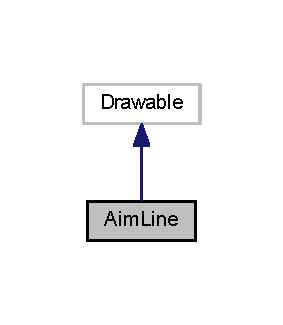
\includegraphics[width=136pt]{class_aim_line__inherit__graph}
\end{center}
\end{figure}


Collaboration diagram for Aim\+Line\+:\nopagebreak
\begin{figure}[H]
\begin{center}
\leavevmode
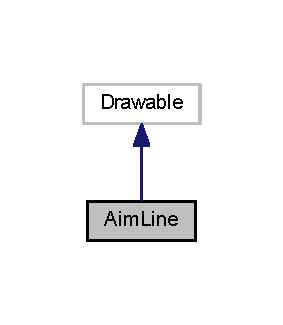
\includegraphics[width=136pt]{class_aim_line__coll__graph}
\end{center}
\end{figure}
\subsection*{Public Member Functions}
\begin{DoxyCompactItemize}
\item 
\mbox{\Hypertarget{class_aim_line_adee034e256147adafb61e5f40ba14f80}\label{class_aim_line_adee034e256147adafb61e5f40ba14f80}} 
\hyperlink{class_aim_line_adee034e256147adafb61e5f40ba14f80}{Aim\+Line} ()
\begin{DoxyCompactList}\small\item\em Default constructor. \end{DoxyCompactList}\item 
\mbox{\Hypertarget{class_aim_line_ab9c038c34f1ccc00acd2731bf5a05dfc}\label{class_aim_line_ab9c038c34f1ccc00acd2731bf5a05dfc}} 
\hyperlink{class_aim_line_ab9c038c34f1ccc00acd2731bf5a05dfc}{$\sim$\+Aim\+Line} ()
\begin{DoxyCompactList}\small\item\em Destructor. \end{DoxyCompactList}\item 
\mbox{\Hypertarget{class_aim_line_ab4ef7f120798090a9d14a85f85238edb}\label{class_aim_line_ab4ef7f120798090a9d14a85f85238edb}} 
float \hyperlink{class_aim_line_ab4ef7f120798090a9d14a85f85238edb}{get\+Multiplier} ()
\begin{DoxyCompactList}\small\item\em get the multiplier value \end{DoxyCompactList}\item 
\mbox{\Hypertarget{class_aim_line_a03bc44a5faf0b438bbb4c5b9df6927ad}\label{class_aim_line_a03bc44a5faf0b438bbb4c5b9df6927ad}} 
sf\+::\+Vector2f \hyperlink{class_aim_line_a03bc44a5faf0b438bbb4c5b9df6927ad}{get\+Dir\+Unit} ()
\begin{DoxyCompactList}\small\item\em get the unit direction vector \end{DoxyCompactList}\item 
void \hyperlink{class_aim_line_ac84b4e6eba6fadc89229357b33d40187}{update} (sf\+::\+Vector2f p\+\_\+\+Target, sf\+::\+Vector2f p\+\_\+\+Start)
\item 
void \hyperlink{class_aim_line_a119d86ded7801300bde99c30ebda6312}{draw} (sf\+::\+Render\+Target \&target, sf\+::\+Render\+States states) const
\end{DoxyCompactItemize}


\subsection{Detailed Description}
A class that creates, updates and draws an aiming reticle. 

\subsection{Member Function Documentation}
\mbox{\Hypertarget{class_aim_line_a119d86ded7801300bde99c30ebda6312}\label{class_aim_line_a119d86ded7801300bde99c30ebda6312}} 
\index{Aim\+Line@{Aim\+Line}!draw@{draw}}
\index{draw@{draw}!Aim\+Line@{Aim\+Line}}
\subsubsection{\texorpdfstring{draw()}{draw()}}
{\footnotesize\ttfamily void Aim\+Line\+::draw (\begin{DoxyParamCaption}\item[{sf\+::\+Render\+Target \&}]{target,  }\item[{sf\+::\+Render\+States}]{states }\end{DoxyParamCaption}) const}

Draw 
\begin{DoxyParams}[1]{Parameters}
\mbox{\tt in,out}  & {\em target} & Render target to draw to \\
\hline
\mbox{\tt in}  & {\em states} & Render state \\
\hline
\end{DoxyParams}
\mbox{\Hypertarget{class_aim_line_ac84b4e6eba6fadc89229357b33d40187}\label{class_aim_line_ac84b4e6eba6fadc89229357b33d40187}} 
\index{Aim\+Line@{Aim\+Line}!update@{update}}
\index{update@{update}!Aim\+Line@{Aim\+Line}}
\subsubsection{\texorpdfstring{update()}{update()}}
{\footnotesize\ttfamily void Aim\+Line\+::update (\begin{DoxyParamCaption}\item[{sf\+::\+Vector2f}]{p\+\_\+\+Target,  }\item[{sf\+::\+Vector2f}]{p\+\_\+\+Start }\end{DoxyParamCaption})}

update the vertices 
\begin{DoxyParams}[1]{Parameters}
\mbox{\tt in}  & {\em p\+\_\+\+Target} & the target position \\
\hline
\mbox{\tt in}  & {\em p\+\_\+\+Start} & the start position \\
\hline
\end{DoxyParams}


The documentation for this class was generated from the following file\+:\begin{DoxyCompactItemize}
\item 
include/\hyperlink{_aim_line_8h}{Aim\+Line.\+h}\end{DoxyCompactItemize}

\hypertarget{class_collision_helper}{}\section{Collision\+Helper Class Reference}
\label{class_collision_helper}\index{Collision\+Helper@{Collision\+Helper}}


A class that contains all the relavent collision checking and resolve methods.  




{\ttfamily \#include $<$Collision\+Helper.\+h$>$}

\subsection*{Static Public Member Functions}
\begin{DoxyCompactItemize}
\item 
static void \hyperlink{class_collision_helper_a57aca4d1a02c1309ca7f80eaecbb4edf}{resolve} (\hyperlink{class_particle}{Particle} \&p\+\_\+\+Particle, sf\+::\+Vector2f p\+\_\+\+Normal, sf\+::\+Vector2i p\+\_\+\+Collision\+Pos)
\item 
static void \hyperlink{class_collision_helper_aec0ce6765c1be0da596147c9df11e69d}{resolve} (\hyperlink{class_dynamic_object}{Dynamic\+Object} \&p\+\_\+\+Dynamic\+Obj, sf\+::\+Vector2f p\+\_\+\+Normal, float p\+\_\+\+Delta\+Time)
\item 
static bool \hyperlink{class_collision_helper_a29f24f7dfa3f65415d415dd23e31bed1}{ray\+Cast} (sf\+::\+Vector2i p\+\_\+\+Start, sf\+::\+Vector2i p\+\_\+\+Target, \hyperlink{class_terrain}{Terrain} \&p\+\_\+\+Terrain, sf\+::\+Vector2i \&p\+\_\+\+Hit\+Pos)
\item 
static bool \hyperlink{class_collision_helper_a98d43fd6735513956419fceb047ac4bd}{A\+A\+B\+Bvs\+Terrain} (sf\+::\+Float\+Rect p\+\_\+\+BB, sf\+::\+Vector2f p\+\_\+\+Pos, \hyperlink{class_terrain}{Terrain} \&p\+\_\+\+Terrain, sf\+::\+Vector2f \&p\+\_\+\+Average\+Unit\+Normal)
\item 
static bool \hyperlink{class_collision_helper_a11469523b5a2b22f10d7d827af1f7e18}{A\+A\+B\+Bvs\+A\+A\+BB} (sf\+::\+Float\+Rect p\+\_\+\+B\+B1, sf\+::\+Vector2f p\+\_\+\+Pos1, sf\+::\+Float\+Rect p\+\_\+\+B\+B2, sf\+::\+Vector2f p\+\_\+\+Pos2)
\item 
static bool \hyperlink{class_collision_helper_a3f3e49b546e37ce2e457dc6582c97adf}{A\+A\+B\+Bvs\+Circle} (sf\+::\+Circle\+Shape p\+\_\+\+Circle1, sf\+::\+Vector2f p\+\_\+\+Pos1, sf\+::\+Float\+Rect p\+\_\+\+B\+B2, sf\+::\+Vector2f p\+\_\+\+Pos2)
\end{DoxyCompactItemize}


\subsection{Detailed Description}
A class that contains all the relavent collision checking and resolve methods. 

\subsection{Member Function Documentation}
\mbox{\Hypertarget{class_collision_helper_a11469523b5a2b22f10d7d827af1f7e18}\label{class_collision_helper_a11469523b5a2b22f10d7d827af1f7e18}} 
\index{Collision\+Helper@{Collision\+Helper}!A\+A\+B\+Bvs\+A\+A\+BB@{A\+A\+B\+Bvs\+A\+A\+BB}}
\index{A\+A\+B\+Bvs\+A\+A\+BB@{A\+A\+B\+Bvs\+A\+A\+BB}!Collision\+Helper@{Collision\+Helper}}
\subsubsection{\texorpdfstring{A\+A\+B\+Bvs\+A\+A\+B\+B()}{AABBvsAABB()}}
{\footnotesize\ttfamily static bool Collision\+Helper\+::\+A\+A\+B\+Bvs\+A\+A\+BB (\begin{DoxyParamCaption}\item[{sf\+::\+Float\+Rect}]{p\+\_\+\+B\+B1,  }\item[{sf\+::\+Vector2f}]{p\+\_\+\+Pos1,  }\item[{sf\+::\+Float\+Rect}]{p\+\_\+\+B\+B2,  }\item[{sf\+::\+Vector2f}]{p\+\_\+\+Pos2 }\end{DoxyParamCaption})\hspace{0.3cm}{\ttfamily [static]}}

Axis Aligned Bounding Box vs Axis Aligned Bounding Box collision check 
\begin{DoxyParams}[1]{Parameters}
\mbox{\tt in}  & {\em p\+\_\+\+B\+B1} & Bounding box 1 \\
\hline
\mbox{\tt in}  & {\em p\+\_\+\+Pos1} & Position of Bounding Box 1 \\
\hline
\mbox{\tt in}  & {\em p\+\_\+\+B\+B2} & Bounding box 2 \\
\hline
\mbox{\tt in}  & {\em p\+\_\+\+Pos2} & Position of Bounding Box 2 \\
\hline
\end{DoxyParams}
\mbox{\Hypertarget{class_collision_helper_a3f3e49b546e37ce2e457dc6582c97adf}\label{class_collision_helper_a3f3e49b546e37ce2e457dc6582c97adf}} 
\index{Collision\+Helper@{Collision\+Helper}!A\+A\+B\+Bvs\+Circle@{A\+A\+B\+Bvs\+Circle}}
\index{A\+A\+B\+Bvs\+Circle@{A\+A\+B\+Bvs\+Circle}!Collision\+Helper@{Collision\+Helper}}
\subsubsection{\texorpdfstring{A\+A\+B\+Bvs\+Circle()}{AABBvsCircle()}}
{\footnotesize\ttfamily static bool Collision\+Helper\+::\+A\+A\+B\+Bvs\+Circle (\begin{DoxyParamCaption}\item[{sf\+::\+Circle\+Shape}]{p\+\_\+\+Circle1,  }\item[{sf\+::\+Vector2f}]{p\+\_\+\+Pos1,  }\item[{sf\+::\+Float\+Rect}]{p\+\_\+\+B\+B2,  }\item[{sf\+::\+Vector2f}]{p\+\_\+\+Pos2 }\end{DoxyParamCaption})\hspace{0.3cm}{\ttfamily [static]}}

Axis Aligned Bounding Box vs Circle collision check 
\begin{DoxyParams}[1]{Parameters}
\mbox{\tt in}  & {\em p\+\_\+\+Circle1} & Circle 1 \\
\hline
\mbox{\tt in}  & {\em p\+\_\+\+Pos1} & Position of Circle 1 \\
\hline
\mbox{\tt in}  & {\em p\+\_\+\+B\+B2} & Bounding box 2 \\
\hline
\mbox{\tt in}  & {\em p\+\_\+\+Pos2} & Position of Bounding Box 2 \\
\hline
\end{DoxyParams}
\mbox{\Hypertarget{class_collision_helper_a98d43fd6735513956419fceb047ac4bd}\label{class_collision_helper_a98d43fd6735513956419fceb047ac4bd}} 
\index{Collision\+Helper@{Collision\+Helper}!A\+A\+B\+Bvs\+Terrain@{A\+A\+B\+Bvs\+Terrain}}
\index{A\+A\+B\+Bvs\+Terrain@{A\+A\+B\+Bvs\+Terrain}!Collision\+Helper@{Collision\+Helper}}
\subsubsection{\texorpdfstring{A\+A\+B\+Bvs\+Terrain()}{AABBvsTerrain()}}
{\footnotesize\ttfamily static bool Collision\+Helper\+::\+A\+A\+B\+Bvs\+Terrain (\begin{DoxyParamCaption}\item[{sf\+::\+Float\+Rect}]{p\+\_\+\+BB,  }\item[{sf\+::\+Vector2f}]{p\+\_\+\+Pos,  }\item[{\hyperlink{class_terrain}{Terrain} \&}]{p\+\_\+\+Terrain,  }\item[{sf\+::\+Vector2f \&}]{p\+\_\+\+Average\+Unit\+Normal }\end{DoxyParamCaption})\hspace{0.3cm}{\ttfamily [static]}}

Axis Aligned Bounding Box vs \hyperlink{class_terrain}{Terrain} collision check 
\begin{DoxyParams}[1]{Parameters}
\mbox{\tt in}  & {\em p\+\_\+\+BB} & Bounding box \\
\hline
\mbox{\tt in}  & {\em p\+\_\+\+Pos} & Position of Bounding Box \\
\hline
\mbox{\tt in}  & {\em p\+\_\+\+Terrain} & The terrain \\
\hline
\mbox{\tt out}  & {\em p\+\_\+\+Average\+Unit\+Normal} & the average unit surface normal of edge points of the bounding box inside the terrain \\
\hline
\end{DoxyParams}
\mbox{\Hypertarget{class_collision_helper_a29f24f7dfa3f65415d415dd23e31bed1}\label{class_collision_helper_a29f24f7dfa3f65415d415dd23e31bed1}} 
\index{Collision\+Helper@{Collision\+Helper}!ray\+Cast@{ray\+Cast}}
\index{ray\+Cast@{ray\+Cast}!Collision\+Helper@{Collision\+Helper}}
\subsubsection{\texorpdfstring{ray\+Cast()}{rayCast()}}
{\footnotesize\ttfamily static bool Collision\+Helper\+::ray\+Cast (\begin{DoxyParamCaption}\item[{sf\+::\+Vector2i}]{p\+\_\+\+Start,  }\item[{sf\+::\+Vector2i}]{p\+\_\+\+Target,  }\item[{\hyperlink{class_terrain}{Terrain} \&}]{p\+\_\+\+Terrain,  }\item[{sf\+::\+Vector2i \&}]{p\+\_\+\+Hit\+Pos }\end{DoxyParamCaption})\hspace{0.3cm}{\ttfamily [static]}}

Iterate from point a to b and return true if the ray hits the terrain 
\begin{DoxyParams}[1]{Parameters}
\mbox{\tt in}  & {\em p\+\_\+\+Start} & Tay start position \\
\hline
\mbox{\tt in}  & {\em p\+\_\+\+Target} & Tay target position \\
\hline
\mbox{\tt in}  & {\em p\+\_\+\+Terrain} & The terrain \\
\hline
\mbox{\tt out}  & {\em p\+\_\+\+Hit\+Pos} & the point at which the ray hits the terrain \\
\hline
\end{DoxyParams}
\mbox{\Hypertarget{class_collision_helper_a57aca4d1a02c1309ca7f80eaecbb4edf}\label{class_collision_helper_a57aca4d1a02c1309ca7f80eaecbb4edf}} 
\index{Collision\+Helper@{Collision\+Helper}!resolve@{resolve}}
\index{resolve@{resolve}!Collision\+Helper@{Collision\+Helper}}
\subsubsection{\texorpdfstring{resolve()}{resolve()}\hspace{0.1cm}{\footnotesize\ttfamily [1/2]}}
{\footnotesize\ttfamily static void Collision\+Helper\+::resolve (\begin{DoxyParamCaption}\item[{\hyperlink{class_particle}{Particle} \&}]{p\+\_\+\+Particle,  }\item[{sf\+::\+Vector2f}]{p\+\_\+\+Normal,  }\item[{sf\+::\+Vector2i}]{p\+\_\+\+Collision\+Pos }\end{DoxyParamCaption})\hspace{0.3cm}{\ttfamily [static]}}

resolve a particle collision 
\begin{DoxyParams}[1]{Parameters}
\mbox{\tt in}  & {\em p\+\_\+\+Particle} & The particle that collided \\
\hline
\mbox{\tt in}  & {\em p\+\_\+\+Normal} & the surface normal \\
\hline
\mbox{\tt in}  & {\em p\+\_\+\+Collision\+Pos} & the point of impact \\
\hline
\end{DoxyParams}
\mbox{\Hypertarget{class_collision_helper_aec0ce6765c1be0da596147c9df11e69d}\label{class_collision_helper_aec0ce6765c1be0da596147c9df11e69d}} 
\index{Collision\+Helper@{Collision\+Helper}!resolve@{resolve}}
\index{resolve@{resolve}!Collision\+Helper@{Collision\+Helper}}
\subsubsection{\texorpdfstring{resolve()}{resolve()}\hspace{0.1cm}{\footnotesize\ttfamily [2/2]}}
{\footnotesize\ttfamily static void Collision\+Helper\+::resolve (\begin{DoxyParamCaption}\item[{\hyperlink{class_dynamic_object}{Dynamic\+Object} \&}]{p\+\_\+\+Dynamic\+Obj,  }\item[{sf\+::\+Vector2f}]{p\+\_\+\+Normal,  }\item[{float}]{p\+\_\+\+Delta\+Time }\end{DoxyParamCaption})\hspace{0.3cm}{\ttfamily [static]}}

resolve a dynamic object collision 
\begin{DoxyParams}[1]{Parameters}
\mbox{\tt in}  & {\em p\+\_\+\+Dynamic\+Obj} & The dynamic object that collided \\
\hline
\mbox{\tt in}  & {\em p\+\_\+\+Normal} & The surface normal \\
\hline
\mbox{\tt in}  & {\em p\+\_\+\+Delta\+Time} & The time elapsed since last frame \\
\hline
\end{DoxyParams}


The documentation for this class was generated from the following file\+:\begin{DoxyCompactItemize}
\item 
include/\hyperlink{_collision_helper_8h}{Collision\+Helper.\+h}\end{DoxyCompactItemize}

\hypertarget{class_dynamic_object}{}\section{Dynamic\+Object Class Reference}
\label{class_dynamic_object}\index{Dynamic\+Object@{Dynamic\+Object}}


A kinematic rectangle that can be affected by forces.  




{\ttfamily \#include $<$Dynamic\+Object.\+h$>$}



Inheritance diagram for Dynamic\+Object\+:\nopagebreak
\begin{figure}[H]
\begin{center}
\leavevmode
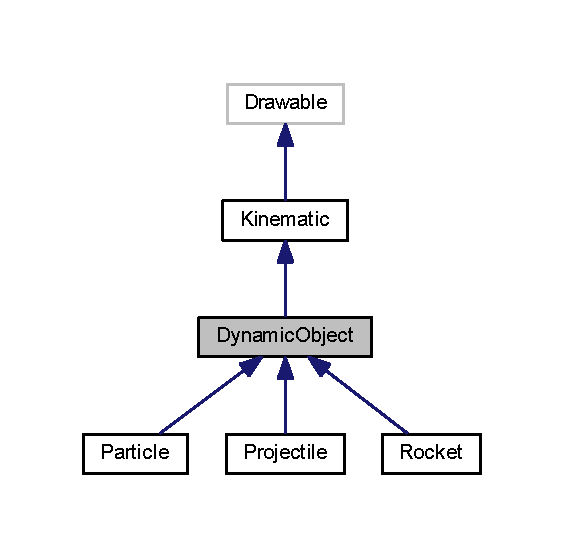
\includegraphics[width=271pt]{class_dynamic_object__inherit__graph}
\end{center}
\end{figure}


Collaboration diagram for Dynamic\+Object\+:\nopagebreak
\begin{figure}[H]
\begin{center}
\leavevmode
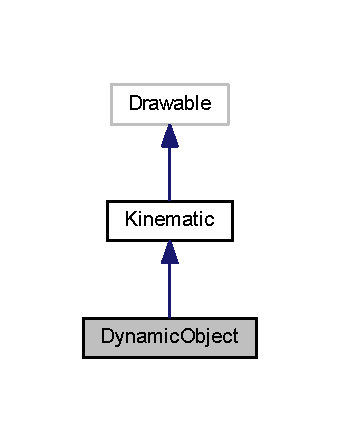
\includegraphics[width=163pt]{class_dynamic_object__coll__graph}
\end{center}
\end{figure}
\subsection*{Public Member Functions}
\begin{DoxyCompactItemize}
\item 
\mbox{\Hypertarget{class_dynamic_object_a50a7adf3d7d1f411ed2aa9a663bfe275}\label{class_dynamic_object_a50a7adf3d7d1f411ed2aa9a663bfe275}} 
\hyperlink{class_dynamic_object_a50a7adf3d7d1f411ed2aa9a663bfe275}{Dynamic\+Object} ()
\begin{DoxyCompactList}\small\item\em Default constructor. \end{DoxyCompactList}\item 
\mbox{\Hypertarget{class_dynamic_object_a149b612e1f0288b115178874bd0cba93}\label{class_dynamic_object_a149b612e1f0288b115178874bd0cba93}} 
\hyperlink{class_dynamic_object_a149b612e1f0288b115178874bd0cba93}{$\sim$\+Dynamic\+Object} ()
\begin{DoxyCompactList}\small\item\em Destructor. \end{DoxyCompactList}\item 
void \hyperlink{class_dynamic_object_a0a0a7729f35bd16156a2fbb75d50ea1c}{set\+Restitution} (float p\+\_\+\+Restitution)
\item 
\mbox{\Hypertarget{class_dynamic_object_a6637df2539ca0aa1a4eed8636863dfac}\label{class_dynamic_object_a6637df2539ca0aa1a4eed8636863dfac}} 
float \hyperlink{class_dynamic_object_a6637df2539ca0aa1a4eed8636863dfac}{get\+Restitution} ()
\begin{DoxyCompactList}\small\item\em get restitution \end{DoxyCompactList}\item 
void \hyperlink{class_dynamic_object_ae3d4fa8bda00ba66b59ade0e01abbec5}{set\+Drag\+Co} (float p\+\_\+\+Drag\+Coefficient)
\item 
\mbox{\Hypertarget{class_dynamic_object_a60373c87f1803073f1e5113913828f4f}\label{class_dynamic_object_a60373c87f1803073f1e5113913828f4f}} 
float \hyperlink{class_dynamic_object_a60373c87f1803073f1e5113913828f4f}{get\+Drag\+Co} ()
\begin{DoxyCompactList}\small\item\em get drag coefficient \end{DoxyCompactList}\item 
void \hyperlink{class_dynamic_object_af6fdf32b8d48afff90e68b2c87d9afe5}{set\+Friction\+Co} (float p\+\_\+\+Fric\+Coefficient)
\item 
\mbox{\Hypertarget{class_dynamic_object_a0c6789df96b1d9007fbc27aa67303408}\label{class_dynamic_object_a0c6789df96b1d9007fbc27aa67303408}} 
float \hyperlink{class_dynamic_object_a0c6789df96b1d9007fbc27aa67303408}{get\+Fric\+Co} ()
\begin{DoxyCompactList}\small\item\em get friction coefficient \end{DoxyCompactList}\item 
\mbox{\Hypertarget{class_dynamic_object_a63350c6fb11deb4ddd568f589fa08b24}\label{class_dynamic_object_a63350c6fb11deb4ddd568f589fa08b24}} 
float \hyperlink{class_dynamic_object_a63350c6fb11deb4ddd568f589fa08b24}{get\+Moment\+Of\+Inertia} ()
\begin{DoxyCompactList}\small\item\em get moment of inertia \end{DoxyCompactList}\item 
\mbox{\Hypertarget{class_dynamic_object_a55b099784c09e8a8dbd8272af92a102d}\label{class_dynamic_object_a55b099784c09e8a8dbd8272af92a102d}} 
float \hyperlink{class_dynamic_object_a55b099784c09e8a8dbd8272af92a102d}{get\+Mass} ()
\begin{DoxyCompactList}\small\item\em get mass \end{DoxyCompactList}\item 
void \hyperlink{class_dynamic_object_a33c22fe97d62f79152c508c03ada948c}{apply\+Force} (sf\+::\+Vector2f p\+\_\+\+Force)
\item 
\mbox{\Hypertarget{class_dynamic_object_ae8948f5724a243df793332b0c8442b0d}\label{class_dynamic_object_ae8948f5724a243df793332b0c8442b0d}} 
sf\+::\+Float\+Rect \hyperlink{class_dynamic_object_ae8948f5724a243df793332b0c8442b0d}{get\+Bound\+Box} ()
\begin{DoxyCompactList}\small\item\em get the bounding box \end{DoxyCompactList}\end{DoxyCompactItemize}
\subsection*{Protected Member Functions}
\begin{DoxyCompactItemize}
\item 
\mbox{\Hypertarget{class_dynamic_object_a1169a5a6cf16738f27a83b2cddcc72f9}\label{class_dynamic_object_a1169a5a6cf16738f27a83b2cddcc72f9}} 
virtual float \hyperlink{class_dynamic_object_a1169a5a6cf16738f27a83b2cddcc72f9}{area} ()=0
\begin{DoxyCompactList}\small\item\em late binding area getter \end{DoxyCompactList}\end{DoxyCompactItemize}
\subsection*{Protected Attributes}
\begin{DoxyCompactItemize}
\item 
\mbox{\Hypertarget{class_dynamic_object_ae418fa977f4547419cda31827c266ae8}\label{class_dynamic_object_ae418fa977f4547419cda31827c266ae8}} 
float \hyperlink{class_dynamic_object_ae418fa977f4547419cda31827c266ae8}{m\+\_\+\+Density} = 1.\+0f
\begin{DoxyCompactList}\small\item\em The density. \end{DoxyCompactList}\item 
\mbox{\Hypertarget{class_dynamic_object_aab95811a0f06dd425a6ecd2a20153083}\label{class_dynamic_object_aab95811a0f06dd425a6ecd2a20153083}} 
float \hyperlink{class_dynamic_object_aab95811a0f06dd425a6ecd2a20153083}{m\+\_\+\+Mass} = 1.\+0f
\begin{DoxyCompactList}\small\item\em The mass. \end{DoxyCompactList}\item 
\mbox{\Hypertarget{class_dynamic_object_ac1fa799a751f1f2b0dd9996f9c2f4c4d}\label{class_dynamic_object_ac1fa799a751f1f2b0dd9996f9c2f4c4d}} 
float \hyperlink{class_dynamic_object_ac1fa799a751f1f2b0dd9996f9c2f4c4d}{m\+\_\+\+Restitution} = 0.\+0f
\begin{DoxyCompactList}\small\item\em The restitution. \end{DoxyCompactList}\item 
\mbox{\Hypertarget{class_dynamic_object_a7721debe06365b091f533b9f1641c2b2}\label{class_dynamic_object_a7721debe06365b091f533b9f1641c2b2}} 
float \hyperlink{class_dynamic_object_a7721debe06365b091f533b9f1641c2b2}{m\+\_\+\+Drag\+Coefficient} = 0.\+0f
\begin{DoxyCompactList}\small\item\em The default drag coefficient. \end{DoxyCompactList}\item 
\mbox{\Hypertarget{class_dynamic_object_aeff80849df69f067cba4b67b8d64019b}\label{class_dynamic_object_aeff80849df69f067cba4b67b8d64019b}} 
float \hyperlink{class_dynamic_object_aeff80849df69f067cba4b67b8d64019b}{m\+\_\+\+Friction\+Coefficient} = 0.\+0f
\begin{DoxyCompactList}\small\item\em The default friction coefficient. \end{DoxyCompactList}\item 
\mbox{\Hypertarget{class_dynamic_object_a860cf85df59fd5d08810d082a43fdab1}\label{class_dynamic_object_a860cf85df59fd5d08810d082a43fdab1}} 
float \hyperlink{class_dynamic_object_a860cf85df59fd5d08810d082a43fdab1}{m\+\_\+\+Moment\+Of\+Inertia} = 1.\+0f
\begin{DoxyCompactList}\small\item\em The default moment of inertia;. \end{DoxyCompactList}\item 
\mbox{\Hypertarget{class_dynamic_object_a7149219cede0b96d7d381b424ae3dd3f}\label{class_dynamic_object_a7149219cede0b96d7d381b424ae3dd3f}} 
sf\+::\+Float\+Rect \hyperlink{class_dynamic_object_a7149219cede0b96d7d381b424ae3dd3f}{m\+\_\+\+Bounding\+Box}
\begin{DoxyCompactList}\small\item\em The bounding box. \end{DoxyCompactList}\end{DoxyCompactItemize}


\subsection{Detailed Description}
A kinematic rectangle that can be affected by forces. 

\subsection{Member Function Documentation}
\mbox{\Hypertarget{class_dynamic_object_a33c22fe97d62f79152c508c03ada948c}\label{class_dynamic_object_a33c22fe97d62f79152c508c03ada948c}} 
\index{Dynamic\+Object@{Dynamic\+Object}!apply\+Force@{apply\+Force}}
\index{apply\+Force@{apply\+Force}!Dynamic\+Object@{Dynamic\+Object}}
\subsubsection{\texorpdfstring{apply\+Force()}{applyForce()}}
{\footnotesize\ttfamily void Dynamic\+Object\+::apply\+Force (\begin{DoxyParamCaption}\item[{sf\+::\+Vector2f}]{p\+\_\+\+Force }\end{DoxyParamCaption})}

apply a force 
\begin{DoxyParams}[1]{Parameters}
\mbox{\tt in}  & {\em p\+\_\+\+Force} & the force to be applied \\
\hline
\end{DoxyParams}
\mbox{\Hypertarget{class_dynamic_object_ae3d4fa8bda00ba66b59ade0e01abbec5}\label{class_dynamic_object_ae3d4fa8bda00ba66b59ade0e01abbec5}} 
\index{Dynamic\+Object@{Dynamic\+Object}!set\+Drag\+Co@{set\+Drag\+Co}}
\index{set\+Drag\+Co@{set\+Drag\+Co}!Dynamic\+Object@{Dynamic\+Object}}
\subsubsection{\texorpdfstring{set\+Drag\+Co()}{setDragCo()}}
{\footnotesize\ttfamily void Dynamic\+Object\+::set\+Drag\+Co (\begin{DoxyParamCaption}\item[{float}]{p\+\_\+\+Drag\+Coefficient }\end{DoxyParamCaption})}

set drag coefficient 
\begin{DoxyParams}[1]{Parameters}
\mbox{\tt in}  & {\em p\+\_\+\+Drag\+Coefficient} & the drag coefficient \\
\hline
\end{DoxyParams}
\mbox{\Hypertarget{class_dynamic_object_af6fdf32b8d48afff90e68b2c87d9afe5}\label{class_dynamic_object_af6fdf32b8d48afff90e68b2c87d9afe5}} 
\index{Dynamic\+Object@{Dynamic\+Object}!set\+Friction\+Co@{set\+Friction\+Co}}
\index{set\+Friction\+Co@{set\+Friction\+Co}!Dynamic\+Object@{Dynamic\+Object}}
\subsubsection{\texorpdfstring{set\+Friction\+Co()}{setFrictionCo()}}
{\footnotesize\ttfamily void Dynamic\+Object\+::set\+Friction\+Co (\begin{DoxyParamCaption}\item[{float}]{p\+\_\+\+Fric\+Coefficient }\end{DoxyParamCaption})}

set friction coefficient 
\begin{DoxyParams}[1]{Parameters}
\mbox{\tt in}  & {\em p\+\_\+\+Fric\+Coefficient} & the friction coefficient \\
\hline
\end{DoxyParams}
\mbox{\Hypertarget{class_dynamic_object_a0a0a7729f35bd16156a2fbb75d50ea1c}\label{class_dynamic_object_a0a0a7729f35bd16156a2fbb75d50ea1c}} 
\index{Dynamic\+Object@{Dynamic\+Object}!set\+Restitution@{set\+Restitution}}
\index{set\+Restitution@{set\+Restitution}!Dynamic\+Object@{Dynamic\+Object}}
\subsubsection{\texorpdfstring{set\+Restitution()}{setRestitution()}}
{\footnotesize\ttfamily void Dynamic\+Object\+::set\+Restitution (\begin{DoxyParamCaption}\item[{float}]{p\+\_\+\+Restitution }\end{DoxyParamCaption})}

set Restitution 
\begin{DoxyParams}[1]{Parameters}
\mbox{\tt in}  & {\em p\+\_\+\+Restitution} & the bounciness value \\
\hline
\end{DoxyParams}


The documentation for this class was generated from the following file\+:\begin{DoxyCompactItemize}
\item 
include/\hyperlink{_dynamic_object_8h}{Dynamic\+Object.\+h}\end{DoxyCompactItemize}

\hypertarget{class_game}{}\section{Game Class Reference}
\label{class_game}\index{Game@{Game}}


A game scene that runs the rocket battle game.  




{\ttfamily \#include $<$Game.\+h$>$}



Inheritance diagram for Game\+:\nopagebreak
\begin{figure}[H]
\begin{center}
\leavevmode
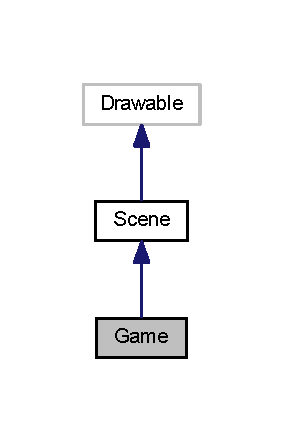
\includegraphics[width=136pt]{class_game__inherit__graph}
\end{center}
\end{figure}


Collaboration diagram for Game\+:\nopagebreak
\begin{figure}[H]
\begin{center}
\leavevmode
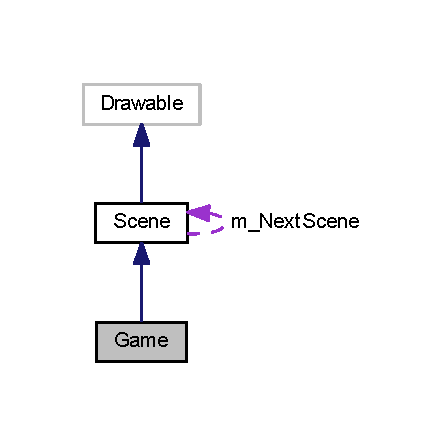
\includegraphics[width=213pt]{class_game__coll__graph}
\end{center}
\end{figure}
\subsection*{Public Member Functions}
\begin{DoxyCompactItemize}
\item 
\hyperlink{class_game_acfaa5dfffe755ef1b09948e9074189b5}{Game} (sf\+::\+Vector2u p\+\_\+\+Window\+Size)
\item 
void \hyperlink{class_game_a6ccc7e91593f06a0e722cc419016a237}{handle\+Keyboard\+Input} (int p\+\_\+\+Key)
\item 
void \hyperlink{class_game_a1c0ddbb7a468997249acbdd6cf2dbe34}{handle\+Mouse\+Input} (sf\+::\+Mouse\+::\+Button p\+\_\+\+Button)
\item 
void \hyperlink{class_game_a3fd12339411955db6a5445ba213ef293}{update} (float p\+\_\+\+Time\+Step)
\item 
void \hyperlink{class_game_a143d1a2f8a527db60f1fe47ab3d854a7}{draw} (sf\+::\+Render\+Target \&target, sf\+::\+Render\+States states) const
\end{DoxyCompactItemize}
\subsection*{Additional Inherited Members}


\subsection{Detailed Description}
A game scene that runs the rocket battle game. 

\subsection{Constructor \& Destructor Documentation}
\mbox{\Hypertarget{class_game_acfaa5dfffe755ef1b09948e9074189b5}\label{class_game_acfaa5dfffe755ef1b09948e9074189b5}} 
\index{Game@{Game}!Game@{Game}}
\index{Game@{Game}!Game@{Game}}
\subsubsection{\texorpdfstring{Game()}{Game()}}
{\footnotesize\ttfamily Game\+::\+Game (\begin{DoxyParamCaption}\item[{sf\+::\+Vector2u}]{p\+\_\+\+Window\+Size }\end{DoxyParamCaption})}

Constructor 
\begin{DoxyParams}[1]{Parameters}
\mbox{\tt in}  & {\em p\+\_\+\+Window\+Size} & Initial window size \\
\hline
\end{DoxyParams}


\subsection{Member Function Documentation}
\mbox{\Hypertarget{class_game_a143d1a2f8a527db60f1fe47ab3d854a7}\label{class_game_a143d1a2f8a527db60f1fe47ab3d854a7}} 
\index{Game@{Game}!draw@{draw}}
\index{draw@{draw}!Game@{Game}}
\subsubsection{\texorpdfstring{draw()}{draw()}}
{\footnotesize\ttfamily void Game\+::draw (\begin{DoxyParamCaption}\item[{sf\+::\+Render\+Target \&}]{target,  }\item[{sf\+::\+Render\+States}]{states }\end{DoxyParamCaption}) const\hspace{0.3cm}{\ttfamily [virtual]}}

Draw 
\begin{DoxyParams}[1]{Parameters}
\mbox{\tt in,out}  & {\em target} & Render target to draw to \\
\hline
\mbox{\tt in}  & {\em states} & Render state \\
\hline
\end{DoxyParams}


Implements \hyperlink{class_scene_ac3fd1d41fa7b7516eeff009de7550552}{Scene}.

\mbox{\Hypertarget{class_game_a6ccc7e91593f06a0e722cc419016a237}\label{class_game_a6ccc7e91593f06a0e722cc419016a237}} 
\index{Game@{Game}!handle\+Keyboard\+Input@{handle\+Keyboard\+Input}}
\index{handle\+Keyboard\+Input@{handle\+Keyboard\+Input}!Game@{Game}}
\subsubsection{\texorpdfstring{handle\+Keyboard\+Input()}{handleKeyboardInput()}}
{\footnotesize\ttfamily void Game\+::handle\+Keyboard\+Input (\begin{DoxyParamCaption}\item[{int}]{p\+\_\+\+Key }\end{DoxyParamCaption})\hspace{0.3cm}{\ttfamily [virtual]}}

handle keyboard events 
\begin{DoxyParams}[1]{Parameters}
\mbox{\tt in}  & {\em p\+\_\+\+Key} & the key that was pressed \\
\hline
\end{DoxyParams}


Implements \hyperlink{class_scene_a182f90e2638c0da6a8ba2eab7cdc73ae}{Scene}.

\mbox{\Hypertarget{class_game_a1c0ddbb7a468997249acbdd6cf2dbe34}\label{class_game_a1c0ddbb7a468997249acbdd6cf2dbe34}} 
\index{Game@{Game}!handle\+Mouse\+Input@{handle\+Mouse\+Input}}
\index{handle\+Mouse\+Input@{handle\+Mouse\+Input}!Game@{Game}}
\subsubsection{\texorpdfstring{handle\+Mouse\+Input()}{handleMouseInput()}}
{\footnotesize\ttfamily void Game\+::handle\+Mouse\+Input (\begin{DoxyParamCaption}\item[{sf\+::\+Mouse\+::\+Button}]{p\+\_\+\+Button }\end{DoxyParamCaption})\hspace{0.3cm}{\ttfamily [virtual]}}

handle mouse button events 
\begin{DoxyParams}[1]{Parameters}
\mbox{\tt in}  & {\em p\+\_\+\+Button} & the button that was pressed \\
\hline
\end{DoxyParams}


Implements \hyperlink{class_scene_ad9240c92a58c4dba4c2409ec8bcff686}{Scene}.

\mbox{\Hypertarget{class_game_a3fd12339411955db6a5445ba213ef293}\label{class_game_a3fd12339411955db6a5445ba213ef293}} 
\index{Game@{Game}!update@{update}}
\index{update@{update}!Game@{Game}}
\subsubsection{\texorpdfstring{update()}{update()}}
{\footnotesize\ttfamily void Game\+::update (\begin{DoxyParamCaption}\item[{float}]{p\+\_\+\+Time\+Step }\end{DoxyParamCaption})\hspace{0.3cm}{\ttfamily [virtual]}}

update the menu 
\begin{DoxyParams}[1]{Parameters}
\mbox{\tt in}  & {\em p\+\_\+\+Time\+Step} & time elapsed since last frame \\
\hline
\end{DoxyParams}


Implements \hyperlink{class_scene_a461d21cd952c7dd0556850a3fc95a760}{Scene}.



The documentation for this class was generated from the following file\+:\begin{DoxyCompactItemize}
\item 
include/\hyperlink{_game_8h}{Game.\+h}\end{DoxyCompactItemize}

\hypertarget{class_game_over}{}\section{Game\+Over Class Reference}
\label{class_game_over}\index{Game\+Over@{Game\+Over}}


A menu scene that displays some useful info and allows you to start the game.  




{\ttfamily \#include $<$Game\+Over.\+h$>$}



Inheritance diagram for Game\+Over\+:\nopagebreak
\begin{figure}[H]
\begin{center}
\leavevmode
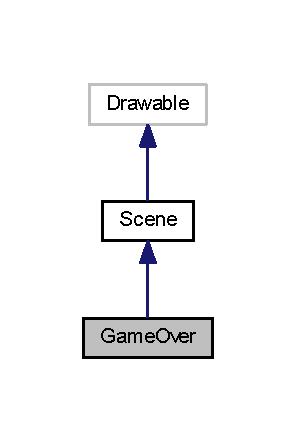
\includegraphics[width=142pt]{class_game_over__inherit__graph}
\end{center}
\end{figure}


Collaboration diagram for Game\+Over\+:\nopagebreak
\begin{figure}[H]
\begin{center}
\leavevmode
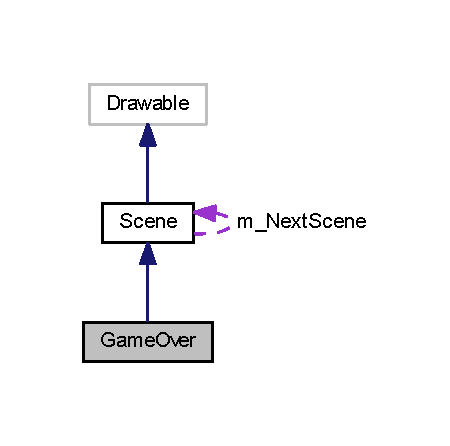
\includegraphics[width=216pt]{class_game_over__coll__graph}
\end{center}
\end{figure}
\subsection*{Public Member Functions}
\begin{DoxyCompactItemize}
\item 
\hyperlink{class_game_over_a03eea2a6051e37b40465cac9377fa7ec}{Game\+Over} (sf\+::\+Vector2u p\+\_\+\+Window\+Size, std\+::string p\+\_\+\+Winner, sf\+::\+Color p\+\_\+\+Color)
\item 
void \hyperlink{class_game_over_aae04263371e8f82199df51de54ef77d1}{handle\+Keyboard\+Input} (int p\+\_\+\+Key)
\item 
void \hyperlink{class_game_over_a83c0cecb3faab5ea8c36272e931006f7}{handle\+Mouse\+Input} (sf\+::\+Mouse\+::\+Button p\+\_\+\+Button)
\item 
void \hyperlink{class_game_over_a6b9465b5c095a1de0e467baf17045fac}{update} (float p\+\_\+\+Time\+Step)
\item 
void \hyperlink{class_game_over_a4792ee9e2b587f98576a8023d34f5f5c}{draw} (sf\+::\+Render\+Target \&target, sf\+::\+Render\+States states) const
\end{DoxyCompactItemize}
\subsection*{Additional Inherited Members}


\subsection{Detailed Description}
A menu scene that displays some useful info and allows you to start the game. 

\subsection{Constructor \& Destructor Documentation}
\mbox{\Hypertarget{class_game_over_a03eea2a6051e37b40465cac9377fa7ec}\label{class_game_over_a03eea2a6051e37b40465cac9377fa7ec}} 
\index{Game\+Over@{Game\+Over}!Game\+Over@{Game\+Over}}
\index{Game\+Over@{Game\+Over}!Game\+Over@{Game\+Over}}
\subsubsection{\texorpdfstring{Game\+Over()}{GameOver()}}
{\footnotesize\ttfamily Game\+Over\+::\+Game\+Over (\begin{DoxyParamCaption}\item[{sf\+::\+Vector2u}]{p\+\_\+\+Window\+Size,  }\item[{std\+::string}]{p\+\_\+\+Winner,  }\item[{sf\+::\+Color}]{p\+\_\+\+Color }\end{DoxyParamCaption})}

Constructor 
\begin{DoxyParams}[1]{Parameters}
\mbox{\tt in}  & {\em p\+\_\+\+Window\+Size} & initial window size \\
\hline
\mbox{\tt in}  & {\em p\+\_\+\+Winner} & the string to be displayed \\
\hline
\mbox{\tt in}  & {\em p\+\_\+\+Color} & the text color \\
\hline
\end{DoxyParams}


\subsection{Member Function Documentation}
\mbox{\Hypertarget{class_game_over_a4792ee9e2b587f98576a8023d34f5f5c}\label{class_game_over_a4792ee9e2b587f98576a8023d34f5f5c}} 
\index{Game\+Over@{Game\+Over}!draw@{draw}}
\index{draw@{draw}!Game\+Over@{Game\+Over}}
\subsubsection{\texorpdfstring{draw()}{draw()}}
{\footnotesize\ttfamily void Game\+Over\+::draw (\begin{DoxyParamCaption}\item[{sf\+::\+Render\+Target \&}]{target,  }\item[{sf\+::\+Render\+States}]{states }\end{DoxyParamCaption}) const\hspace{0.3cm}{\ttfamily [virtual]}}

Draw 
\begin{DoxyParams}[1]{Parameters}
\mbox{\tt in,out}  & {\em target} & Render target to draw to \\
\hline
\mbox{\tt in}  & {\em states} & Render state \\
\hline
\end{DoxyParams}


Implements \hyperlink{class_scene_ac3fd1d41fa7b7516eeff009de7550552}{Scene}.

\mbox{\Hypertarget{class_game_over_aae04263371e8f82199df51de54ef77d1}\label{class_game_over_aae04263371e8f82199df51de54ef77d1}} 
\index{Game\+Over@{Game\+Over}!handle\+Keyboard\+Input@{handle\+Keyboard\+Input}}
\index{handle\+Keyboard\+Input@{handle\+Keyboard\+Input}!Game\+Over@{Game\+Over}}
\subsubsection{\texorpdfstring{handle\+Keyboard\+Input()}{handleKeyboardInput()}}
{\footnotesize\ttfamily void Game\+Over\+::handle\+Keyboard\+Input (\begin{DoxyParamCaption}\item[{int}]{p\+\_\+\+Key }\end{DoxyParamCaption})\hspace{0.3cm}{\ttfamily [virtual]}}

handle keyboard events 
\begin{DoxyParams}[1]{Parameters}
\mbox{\tt in}  & {\em p\+\_\+\+Key} & the key that was pressed \\
\hline
\end{DoxyParams}


Implements \hyperlink{class_scene_a182f90e2638c0da6a8ba2eab7cdc73ae}{Scene}.

\mbox{\Hypertarget{class_game_over_a83c0cecb3faab5ea8c36272e931006f7}\label{class_game_over_a83c0cecb3faab5ea8c36272e931006f7}} 
\index{Game\+Over@{Game\+Over}!handle\+Mouse\+Input@{handle\+Mouse\+Input}}
\index{handle\+Mouse\+Input@{handle\+Mouse\+Input}!Game\+Over@{Game\+Over}}
\subsubsection{\texorpdfstring{handle\+Mouse\+Input()}{handleMouseInput()}}
{\footnotesize\ttfamily void Game\+Over\+::handle\+Mouse\+Input (\begin{DoxyParamCaption}\item[{sf\+::\+Mouse\+::\+Button}]{p\+\_\+\+Button }\end{DoxyParamCaption})\hspace{0.3cm}{\ttfamily [virtual]}}

handle mouse button events 
\begin{DoxyParams}[1]{Parameters}
\mbox{\tt in}  & {\em p\+\_\+\+Button} & the button that was pressed \\
\hline
\end{DoxyParams}


Implements \hyperlink{class_scene_ad9240c92a58c4dba4c2409ec8bcff686}{Scene}.

\mbox{\Hypertarget{class_game_over_a6b9465b5c095a1de0e467baf17045fac}\label{class_game_over_a6b9465b5c095a1de0e467baf17045fac}} 
\index{Game\+Over@{Game\+Over}!update@{update}}
\index{update@{update}!Game\+Over@{Game\+Over}}
\subsubsection{\texorpdfstring{update()}{update()}}
{\footnotesize\ttfamily void Game\+Over\+::update (\begin{DoxyParamCaption}\item[{float}]{p\+\_\+\+Time\+Step }\end{DoxyParamCaption})\hspace{0.3cm}{\ttfamily [virtual]}}

update the menu 
\begin{DoxyParams}[1]{Parameters}
\mbox{\tt in}  & {\em p\+\_\+\+Time\+Step} & time elapsed since last frame \\
\hline
\end{DoxyParams}


Implements \hyperlink{class_scene_a461d21cd952c7dd0556850a3fc95a760}{Scene}.



The documentation for this class was generated from the following file\+:\begin{DoxyCompactItemize}
\item 
include/\hyperlink{_game_over_8h}{Game\+Over.\+h}\end{DoxyCompactItemize}

\hypertarget{class_kinematic}{}\section{Kinematic Class Reference}
\label{class_kinematic}\index{Kinematic@{Kinematic}}


A class that provides methods to create motion using position, velocity and acceleration.  




{\ttfamily \#include $<$Kinematic.\+h$>$}



Inheritance diagram for Kinematic\+:\nopagebreak
\begin{figure}[H]
\begin{center}
\leavevmode
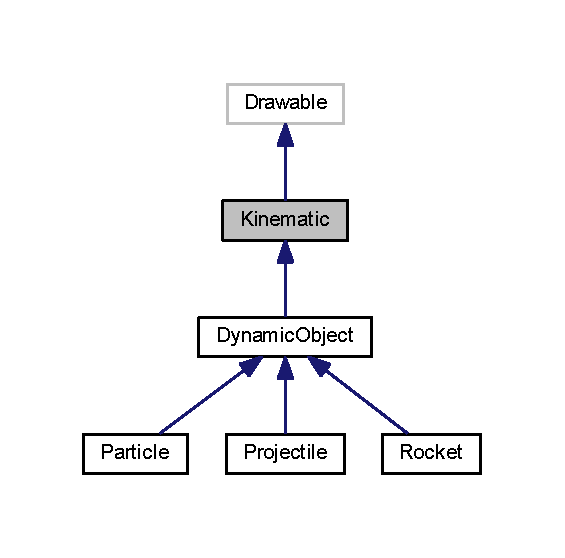
\includegraphics[width=271pt]{class_kinematic__inherit__graph}
\end{center}
\end{figure}


Collaboration diagram for Kinematic\+:\nopagebreak
\begin{figure}[H]
\begin{center}
\leavevmode
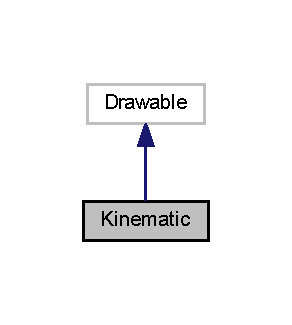
\includegraphics[width=140pt]{class_kinematic__coll__graph}
\end{center}
\end{figure}
\subsection*{Public Member Functions}
\begin{DoxyCompactItemize}
\item 
\mbox{\Hypertarget{class_kinematic_a0265e971c0ac4a847df7d625553becc2}\label{class_kinematic_a0265e971c0ac4a847df7d625553becc2}} 
\hyperlink{class_kinematic_a0265e971c0ac4a847df7d625553becc2}{Kinematic} ()
\begin{DoxyCompactList}\small\item\em Default constructor. \end{DoxyCompactList}\item 
\mbox{\Hypertarget{class_kinematic_ad2e5f972b7bd6e6919473f5fd38cf355}\label{class_kinematic_ad2e5f972b7bd6e6919473f5fd38cf355}} 
\hyperlink{class_kinematic_ad2e5f972b7bd6e6919473f5fd38cf355}{$\sim$\+Kinematic} ()
\begin{DoxyCompactList}\small\item\em Destructor. \end{DoxyCompactList}\item 
\mbox{\Hypertarget{class_kinematic_a19b6a52bb1017eb04b8f6d1b349ee00f}\label{class_kinematic_a19b6a52bb1017eb04b8f6d1b349ee00f}} 
sf\+::\+Vector2f \hyperlink{class_kinematic_a19b6a52bb1017eb04b8f6d1b349ee00f}{get\+Position} ()
\begin{DoxyCompactList}\small\item\em Get current position. \end{DoxyCompactList}\item 
\mbox{\Hypertarget{class_kinematic_a4bddbed2a08c93538ef982b6420f39c6}\label{class_kinematic_a4bddbed2a08c93538ef982b6420f39c6}} 
sf\+::\+Vector2f \hyperlink{class_kinematic_a4bddbed2a08c93538ef982b6420f39c6}{get\+Velocity} ()
\begin{DoxyCompactList}\small\item\em Get current velocity. \end{DoxyCompactList}\item 
\mbox{\Hypertarget{class_kinematic_a4ff84ca5c4d11dae399ea8abc8b25e69}\label{class_kinematic_a4ff84ca5c4d11dae399ea8abc8b25e69}} 
sf\+::\+Vector2f \hyperlink{class_kinematic_a4ff84ca5c4d11dae399ea8abc8b25e69}{get\+Acceleration} ()
\begin{DoxyCompactList}\small\item\em Get current acceleration. \end{DoxyCompactList}\item 
\mbox{\Hypertarget{class_kinematic_a477df46feabc6a17eaae68f860b23e07}\label{class_kinematic_a477df46feabc6a17eaae68f860b23e07}} 
float \hyperlink{class_kinematic_a477df46feabc6a17eaae68f860b23e07}{get\+Angular\+Vel} ()
\begin{DoxyCompactList}\small\item\em Get current angular velocity. \end{DoxyCompactList}\item 
void \hyperlink{class_kinematic_acca21f5a492ef8cea9aa168e2bd1aada}{apply\+Acceleration} (sf\+::\+Vector2f p\+\_\+\+Acceleration)
\item 
void \hyperlink{class_kinematic_afcf0ed9a3b711fd149cb64cc66711c6c}{set\+Position} (sf\+::\+Vector2f p\+\_\+\+Position)
\item 
void \hyperlink{class_kinematic_ad32a87fafb92696178ec3edf69b4657c}{set\+Velocity} (sf\+::\+Vector2f p\+\_\+\+Velocity)
\item 
void \hyperlink{class_kinematic_aafc7bfadfcbbfe84d58162063f0ae94a}{poly\+Update} (float p\+\_\+\+Delta\+Time)
\item 
virtual void \hyperlink{class_kinematic_a5d403bfe970efc1f0cebc872e3e2898b}{draw} (sf\+::\+Render\+Target \&target, sf\+::\+Render\+States states) const =0
\end{DoxyCompactItemize}
\subsection*{Protected Member Functions}
\begin{DoxyCompactItemize}
\item 
\mbox{\Hypertarget{class_kinematic_a99f7c1c609633a7bd5970d5a4f7e7c51}\label{class_kinematic_a99f7c1c609633a7bd5970d5a4f7e7c51}} 
virtual void \hyperlink{class_kinematic_a99f7c1c609633a7bd5970d5a4f7e7c51}{update} ()=0
\begin{DoxyCompactList}\small\item\em late binding update function to update child objects \end{DoxyCompactList}\end{DoxyCompactItemize}
\subsection*{Protected Attributes}
\begin{DoxyCompactItemize}
\item 
\mbox{\Hypertarget{class_kinematic_aa25918dd272373d7ae0451d3b660feb7}\label{class_kinematic_aa25918dd272373d7ae0451d3b660feb7}} 
sf\+::\+Vector2f \hyperlink{class_kinematic_aa25918dd272373d7ae0451d3b660feb7}{m\+\_\+\+Position} = sf\+::\+Vector2f(0.\+0f, 0.\+0f)
\begin{DoxyCompactList}\small\item\em Position of object. \end{DoxyCompactList}\item 
\mbox{\Hypertarget{class_kinematic_a73a21594befb8538e7de53f53dc52be6}\label{class_kinematic_a73a21594befb8538e7de53f53dc52be6}} 
sf\+::\+Vector2f \hyperlink{class_kinematic_a73a21594befb8538e7de53f53dc52be6}{m\+\_\+\+Velocity} = sf\+::\+Vector2f(0.\+0f, 0.\+0f)
\begin{DoxyCompactList}\small\item\em Velocity of object. \end{DoxyCompactList}\item 
\mbox{\Hypertarget{class_kinematic_a30a099a276dbd1aee8f0ef20a63193dc}\label{class_kinematic_a30a099a276dbd1aee8f0ef20a63193dc}} 
sf\+::\+Vector2f \hyperlink{class_kinematic_a30a099a276dbd1aee8f0ef20a63193dc}{m\+\_\+\+Acceleration} = sf\+::\+Vector2f(0.\+0f, 0.\+0f)
\begin{DoxyCompactList}\small\item\em Acceleration of object. \end{DoxyCompactList}\item 
\mbox{\Hypertarget{class_kinematic_a3148fd60ff6257f32a6e3d7042d535d5}\label{class_kinematic_a3148fd60ff6257f32a6e3d7042d535d5}} 
float \hyperlink{class_kinematic_a3148fd60ff6257f32a6e3d7042d535d5}{m\+\_\+\+Rotation} = 0.\+0f
\begin{DoxyCompactList}\small\item\em Rotation of object. \end{DoxyCompactList}\item 
\mbox{\Hypertarget{class_kinematic_afc52c98bc512eef24a46fc29fe6fd012}\label{class_kinematic_afc52c98bc512eef24a46fc29fe6fd012}} 
float \hyperlink{class_kinematic_afc52c98bc512eef24a46fc29fe6fd012}{m\+\_\+\+Angular\+Velocity} = 0.\+0f
\begin{DoxyCompactList}\small\item\em Angular velocity of object. \end{DoxyCompactList}\item 
\mbox{\Hypertarget{class_kinematic_a2f934f9423f65affa32479958694e4ad}\label{class_kinematic_a2f934f9423f65affa32479958694e4ad}} 
float \hyperlink{class_kinematic_a2f934f9423f65affa32479958694e4ad}{m\+\_\+\+Angular\+Acceleration} = 0.\+0f
\begin{DoxyCompactList}\small\item\em Angular acceleration Rotation of object. \end{DoxyCompactList}\end{DoxyCompactItemize}


\subsection{Detailed Description}
A class that provides methods to create motion using position, velocity and acceleration. 

\subsection{Member Function Documentation}
\mbox{\Hypertarget{class_kinematic_acca21f5a492ef8cea9aa168e2bd1aada}\label{class_kinematic_acca21f5a492ef8cea9aa168e2bd1aada}} 
\index{Kinematic@{Kinematic}!apply\+Acceleration@{apply\+Acceleration}}
\index{apply\+Acceleration@{apply\+Acceleration}!Kinematic@{Kinematic}}
\subsubsection{\texorpdfstring{apply\+Acceleration()}{applyAcceleration()}}
{\footnotesize\ttfamily void Kinematic\+::apply\+Acceleration (\begin{DoxyParamCaption}\item[{sf\+::\+Vector2f}]{p\+\_\+\+Acceleration }\end{DoxyParamCaption})}

Apply an acceleration 
\begin{DoxyParams}[1]{Parameters}
\mbox{\tt in}  & {\em p\+\_\+\+Acceleration} & Acceleration \\
\hline
\end{DoxyParams}
\mbox{\Hypertarget{class_kinematic_a5d403bfe970efc1f0cebc872e3e2898b}\label{class_kinematic_a5d403bfe970efc1f0cebc872e3e2898b}} 
\index{Kinematic@{Kinematic}!draw@{draw}}
\index{draw@{draw}!Kinematic@{Kinematic}}
\subsubsection{\texorpdfstring{draw()}{draw()}}
{\footnotesize\ttfamily virtual void Kinematic\+::draw (\begin{DoxyParamCaption}\item[{sf\+::\+Render\+Target \&}]{target,  }\item[{sf\+::\+Render\+States}]{states }\end{DoxyParamCaption}) const\hspace{0.3cm}{\ttfamily [pure virtual]}}

Draw 
\begin{DoxyParams}[1]{Parameters}
\mbox{\tt in,out}  & {\em target} & Render target to draw to \\
\hline
\mbox{\tt in}  & {\em states} & Render state \\
\hline
\end{DoxyParams}


Implemented in \hyperlink{class_rocket_a4b83a058408ee42ea77248dd8f0d3339}{Rocket}, \hyperlink{class_particle_a57316a997dbf6b060ec989c059ba9616}{Particle}, and \hyperlink{class_projectile_ac61792f1670310d35ecec906ab5ada9d}{Projectile}.

\mbox{\Hypertarget{class_kinematic_aafc7bfadfcbbfe84d58162063f0ae94a}\label{class_kinematic_aafc7bfadfcbbfe84d58162063f0ae94a}} 
\index{Kinematic@{Kinematic}!poly\+Update@{poly\+Update}}
\index{poly\+Update@{poly\+Update}!Kinematic@{Kinematic}}
\subsubsection{\texorpdfstring{poly\+Update()}{polyUpdate()}}
{\footnotesize\ttfamily void Kinematic\+::poly\+Update (\begin{DoxyParamCaption}\item[{float}]{p\+\_\+\+Delta\+Time }\end{DoxyParamCaption})}

Update function that calls the child\textquotesingle{}s update function, intergrates and resets acceleration to 0 
\begin{DoxyParams}[1]{Parameters}
\mbox{\tt in}  & {\em p\+\_\+\+Delta\+Time} & elapsed time \\
\hline
\end{DoxyParams}
\mbox{\Hypertarget{class_kinematic_afcf0ed9a3b711fd149cb64cc66711c6c}\label{class_kinematic_afcf0ed9a3b711fd149cb64cc66711c6c}} 
\index{Kinematic@{Kinematic}!set\+Position@{set\+Position}}
\index{set\+Position@{set\+Position}!Kinematic@{Kinematic}}
\subsubsection{\texorpdfstring{set\+Position()}{setPosition()}}
{\footnotesize\ttfamily void Kinematic\+::set\+Position (\begin{DoxyParamCaption}\item[{sf\+::\+Vector2f}]{p\+\_\+\+Position }\end{DoxyParamCaption})}

Set position 
\begin{DoxyParams}[1]{Parameters}
\mbox{\tt in}  & {\em p\+\_\+\+Position} & position \\
\hline
\end{DoxyParams}
\mbox{\Hypertarget{class_kinematic_ad32a87fafb92696178ec3edf69b4657c}\label{class_kinematic_ad32a87fafb92696178ec3edf69b4657c}} 
\index{Kinematic@{Kinematic}!set\+Velocity@{set\+Velocity}}
\index{set\+Velocity@{set\+Velocity}!Kinematic@{Kinematic}}
\subsubsection{\texorpdfstring{set\+Velocity()}{setVelocity()}}
{\footnotesize\ttfamily void Kinematic\+::set\+Velocity (\begin{DoxyParamCaption}\item[{sf\+::\+Vector2f}]{p\+\_\+\+Velocity }\end{DoxyParamCaption})}

Set velocity 
\begin{DoxyParams}[1]{Parameters}
\mbox{\tt in}  & {\em p\+\_\+\+Velocity} & velocity \\
\hline
\end{DoxyParams}


The documentation for this class was generated from the following file\+:\begin{DoxyCompactItemize}
\item 
include/\hyperlink{_kinematic_8h}{Kinematic.\+h}\end{DoxyCompactItemize}

\hypertarget{class_menu}{}\section{Menu Class Reference}
\label{class_menu}\index{Menu@{Menu}}


A menu scene that displays some useful info and allows you to start the game.  




{\ttfamily \#include $<$Menu.\+h$>$}



Inheritance diagram for Menu\+:\nopagebreak
\begin{figure}[H]
\begin{center}
\leavevmode
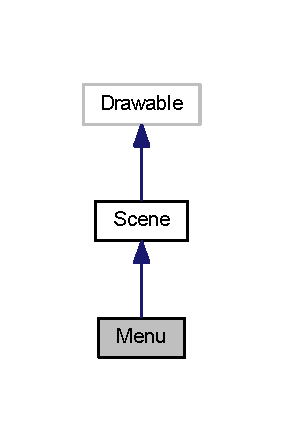
\includegraphics[width=136pt]{class_menu__inherit__graph}
\end{center}
\end{figure}


Collaboration diagram for Menu\+:\nopagebreak
\begin{figure}[H]
\begin{center}
\leavevmode
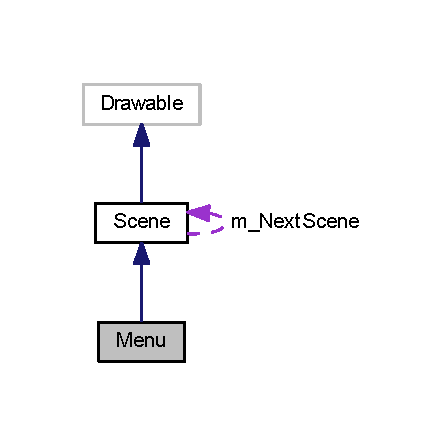
\includegraphics[width=213pt]{class_menu__coll__graph}
\end{center}
\end{figure}
\subsection*{Public Member Functions}
\begin{DoxyCompactItemize}
\item 
\hyperlink{class_menu_a9d1e0ed519f27305e1e5a7237f1586bb}{Menu} (sf\+::\+Vector2u p\+\_\+\+Window\+Size)
\item 
\mbox{\Hypertarget{class_menu_a831387f51358cfb88cd018e1777bc980}\label{class_menu_a831387f51358cfb88cd018e1777bc980}} 
\hyperlink{class_menu_a831387f51358cfb88cd018e1777bc980}{$\sim$\+Menu} ()
\begin{DoxyCompactList}\small\item\em Destructor. \end{DoxyCompactList}\item 
void \hyperlink{class_menu_a2ebc63a5e64b90dcfae4284e7f7f4be6}{handle\+Keyboard\+Input} (int p\+\_\+\+Key)
\item 
void \hyperlink{class_menu_a4f99fe96e47268bd4561df0c8faa23c8}{handle\+Mouse\+Input} (sf\+::\+Mouse\+::\+Button p\+\_\+\+Button)
\item 
void \hyperlink{class_menu_a8043b25a060513367b0e286d3ae397d2}{update} (float p\+\_\+\+Time\+Step)
\item 
void \hyperlink{class_menu_aa0e69963ee402f3559680e5a691b03fd}{draw} (sf\+::\+Render\+Target \&target, sf\+::\+Render\+States states) const
\end{DoxyCompactItemize}
\subsection*{Additional Inherited Members}


\subsection{Detailed Description}
A menu scene that displays some useful info and allows you to start the game. 

\subsection{Constructor \& Destructor Documentation}
\mbox{\Hypertarget{class_menu_a9d1e0ed519f27305e1e5a7237f1586bb}\label{class_menu_a9d1e0ed519f27305e1e5a7237f1586bb}} 
\index{Menu@{Menu}!Menu@{Menu}}
\index{Menu@{Menu}!Menu@{Menu}}
\subsubsection{\texorpdfstring{Menu()}{Menu()}}
{\footnotesize\ttfamily Menu\+::\+Menu (\begin{DoxyParamCaption}\item[{sf\+::\+Vector2u}]{p\+\_\+\+Window\+Size }\end{DoxyParamCaption})}

Constructor 
\begin{DoxyParams}[1]{Parameters}
\mbox{\tt in}  & {\em p\+\_\+\+Window\+Size} & initial window size \\
\hline
\end{DoxyParams}


\subsection{Member Function Documentation}
\mbox{\Hypertarget{class_menu_aa0e69963ee402f3559680e5a691b03fd}\label{class_menu_aa0e69963ee402f3559680e5a691b03fd}} 
\index{Menu@{Menu}!draw@{draw}}
\index{draw@{draw}!Menu@{Menu}}
\subsubsection{\texorpdfstring{draw()}{draw()}}
{\footnotesize\ttfamily void Menu\+::draw (\begin{DoxyParamCaption}\item[{sf\+::\+Render\+Target \&}]{target,  }\item[{sf\+::\+Render\+States}]{states }\end{DoxyParamCaption}) const\hspace{0.3cm}{\ttfamily [virtual]}}

Draw 
\begin{DoxyParams}[1]{Parameters}
\mbox{\tt in,out}  & {\em target} & Render target to draw to \\
\hline
\mbox{\tt in}  & {\em states} & Render state \\
\hline
\end{DoxyParams}


Implements \hyperlink{class_scene_ac3fd1d41fa7b7516eeff009de7550552}{Scene}.

\mbox{\Hypertarget{class_menu_a2ebc63a5e64b90dcfae4284e7f7f4be6}\label{class_menu_a2ebc63a5e64b90dcfae4284e7f7f4be6}} 
\index{Menu@{Menu}!handle\+Keyboard\+Input@{handle\+Keyboard\+Input}}
\index{handle\+Keyboard\+Input@{handle\+Keyboard\+Input}!Menu@{Menu}}
\subsubsection{\texorpdfstring{handle\+Keyboard\+Input()}{handleKeyboardInput()}}
{\footnotesize\ttfamily void Menu\+::handle\+Keyboard\+Input (\begin{DoxyParamCaption}\item[{int}]{p\+\_\+\+Key }\end{DoxyParamCaption})\hspace{0.3cm}{\ttfamily [virtual]}}

handle keyboard events 
\begin{DoxyParams}[1]{Parameters}
\mbox{\tt in}  & {\em p\+\_\+\+Key} & the key that was pressed \\
\hline
\end{DoxyParams}


Implements \hyperlink{class_scene_a182f90e2638c0da6a8ba2eab7cdc73ae}{Scene}.

\mbox{\Hypertarget{class_menu_a4f99fe96e47268bd4561df0c8faa23c8}\label{class_menu_a4f99fe96e47268bd4561df0c8faa23c8}} 
\index{Menu@{Menu}!handle\+Mouse\+Input@{handle\+Mouse\+Input}}
\index{handle\+Mouse\+Input@{handle\+Mouse\+Input}!Menu@{Menu}}
\subsubsection{\texorpdfstring{handle\+Mouse\+Input()}{handleMouseInput()}}
{\footnotesize\ttfamily void Menu\+::handle\+Mouse\+Input (\begin{DoxyParamCaption}\item[{sf\+::\+Mouse\+::\+Button}]{p\+\_\+\+Button }\end{DoxyParamCaption})\hspace{0.3cm}{\ttfamily [virtual]}}

handle mouse button events 
\begin{DoxyParams}[1]{Parameters}
\mbox{\tt in}  & {\em p\+\_\+\+Button} & the button that was pressed \\
\hline
\end{DoxyParams}


Implements \hyperlink{class_scene_ad9240c92a58c4dba4c2409ec8bcff686}{Scene}.

\mbox{\Hypertarget{class_menu_a8043b25a060513367b0e286d3ae397d2}\label{class_menu_a8043b25a060513367b0e286d3ae397d2}} 
\index{Menu@{Menu}!update@{update}}
\index{update@{update}!Menu@{Menu}}
\subsubsection{\texorpdfstring{update()}{update()}}
{\footnotesize\ttfamily void Menu\+::update (\begin{DoxyParamCaption}\item[{float}]{p\+\_\+\+Time\+Step }\end{DoxyParamCaption})\hspace{0.3cm}{\ttfamily [virtual]}}

update the menu 
\begin{DoxyParams}[1]{Parameters}
\mbox{\tt in}  & {\em p\+\_\+\+Time\+Step} & time elapsed since last frame \\
\hline
\end{DoxyParams}


Implements \hyperlink{class_scene_a461d21cd952c7dd0556850a3fc95a760}{Scene}.



The documentation for this class was generated from the following file\+:\begin{DoxyCompactItemize}
\item 
include/\hyperlink{_menu_8h}{Menu.\+h}\end{DoxyCompactItemize}

\hypertarget{class_particle}{}\section{Particle Class Reference}
\label{class_particle}\index{Particle@{Particle}}


A dynamic object that keeps track of how long it exists for and its previous position.  




{\ttfamily \#include $<$Particle.\+h$>$}



Inheritance diagram for Particle\+:\nopagebreak
\begin{figure}[H]
\begin{center}
\leavevmode
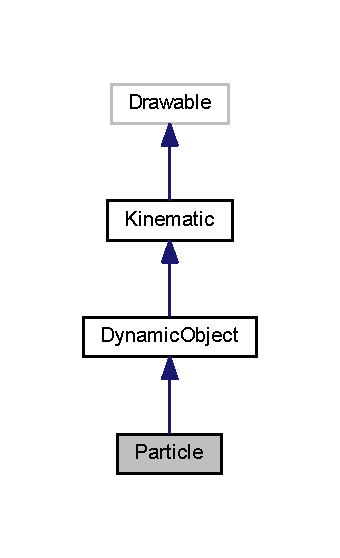
\includegraphics[width=163pt]{class_particle__inherit__graph}
\end{center}
\end{figure}


Collaboration diagram for Particle\+:\nopagebreak
\begin{figure}[H]
\begin{center}
\leavevmode
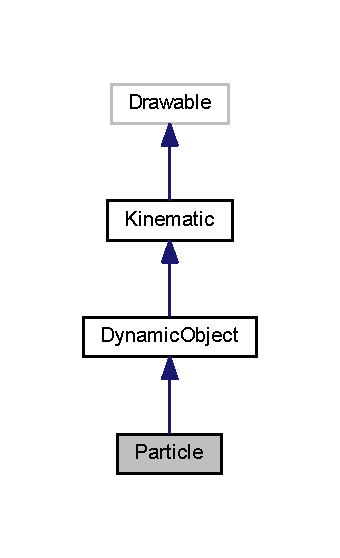
\includegraphics[width=163pt]{class_particle__coll__graph}
\end{center}
\end{figure}
\subsection*{Public Member Functions}
\begin{DoxyCompactItemize}
\item 
\hyperlink{class_particle_ac4b406b1462a981e7a0e430b7592e049}{Particle} (float p\+\_\+\+Life\+Time, sf\+::\+Vector2f p\+\_\+\+Accel, sf\+::\+Vector2f p\+\_\+\+Vel, sf\+::\+Vector2f p\+\_\+\+Pos, float p\+\_\+\+Restitution, float p\+\_\+\+Density, float p\+\_\+\+Drag\+Co)
\item 
void \hyperlink{class_particle_a5a10e04871f4948c80820c79121e28a5}{set\+Last\+Pos} (sf\+::\+Vector2f p\+\_\+\+Position)
\item 
\mbox{\Hypertarget{class_particle_a637683e83cbdf74ea92e8f01653e9156}\label{class_particle_a637683e83cbdf74ea92e8f01653e9156}} 
sf\+::\+Vector2f \hyperlink{class_particle_a637683e83cbdf74ea92e8f01653e9156}{get\+Last\+Pos} ()
\begin{DoxyCompactList}\small\item\em Get the last position. \end{DoxyCompactList}\item 
void \hyperlink{class_particle_a5a7e1ab519e58d9599cb6de75502f60f}{set\+Life} (float p\+\_\+\+Time)
\item 
\mbox{\Hypertarget{class_particle_a59bbb8b7047dfa0c22fcdc37999fb278}\label{class_particle_a59bbb8b7047dfa0c22fcdc37999fb278}} 
float \hyperlink{class_particle_a59bbb8b7047dfa0c22fcdc37999fb278}{get\+Life} ()
\begin{DoxyCompactList}\small\item\em get the current life time \end{DoxyCompactList}\item 
\mbox{\Hypertarget{class_particle_a979da9e9c175ca4915aa2e074e844d6d}\label{class_particle_a979da9e9c175ca4915aa2e074e844d6d}} 
float \hyperlink{class_particle_a979da9e9c175ca4915aa2e074e844d6d}{area} ()
\begin{DoxyCompactList}\small\item\em return the area of a particle \end{DoxyCompactList}\item 
void \hyperlink{class_particle_a57316a997dbf6b060ec989c059ba9616}{draw} (sf\+::\+Render\+Target \&target, sf\+::\+Render\+States states) const
\item 
\mbox{\Hypertarget{class_particle_ad030d0fe7b88cf81744b127c99244ff4}\label{class_particle_ad030d0fe7b88cf81744b127c99244ff4}} 
\hyperlink{class_particle_ad030d0fe7b88cf81744b127c99244ff4}{$\sim$\+Particle} ()
\begin{DoxyCompactList}\small\item\em Destructor. \end{DoxyCompactList}\end{DoxyCompactItemize}
\subsection*{Protected Attributes}
\begin{DoxyCompactItemize}
\item 
\mbox{\Hypertarget{class_particle_a1b55980ef25543065a4565224d3cb8d2}\label{class_particle_a1b55980ef25543065a4565224d3cb8d2}} 
float \hyperlink{class_particle_a1b55980ef25543065a4565224d3cb8d2}{m\+\_\+\+Life\+Time} = 0.\+0f
\begin{DoxyCompactList}\small\item\em The time left. \end{DoxyCompactList}\item 
\mbox{\Hypertarget{class_particle_a8d9af488a566382cc890e707212bd272}\label{class_particle_a8d9af488a566382cc890e707212bd272}} 
sf\+::\+Vector2f \hyperlink{class_particle_a8d9af488a566382cc890e707212bd272}{m\+\_\+\+Last\+Position} = sf\+::\+Vector2f(0.\+0f, 0.\+0f)
\begin{DoxyCompactList}\small\item\em The particles last position. \end{DoxyCompactList}\end{DoxyCompactItemize}
\subsection*{Additional Inherited Members}


\subsection{Detailed Description}
A dynamic object that keeps track of how long it exists for and its previous position. 

\subsection{Constructor \& Destructor Documentation}
\mbox{\Hypertarget{class_particle_ac4b406b1462a981e7a0e430b7592e049}\label{class_particle_ac4b406b1462a981e7a0e430b7592e049}} 
\index{Particle@{Particle}!Particle@{Particle}}
\index{Particle@{Particle}!Particle@{Particle}}
\subsubsection{\texorpdfstring{Particle()}{Particle()}}
{\footnotesize\ttfamily Particle\+::\+Particle (\begin{DoxyParamCaption}\item[{float}]{p\+\_\+\+Life\+Time,  }\item[{sf\+::\+Vector2f}]{p\+\_\+\+Accel,  }\item[{sf\+::\+Vector2f}]{p\+\_\+\+Vel,  }\item[{sf\+::\+Vector2f}]{p\+\_\+\+Pos,  }\item[{float}]{p\+\_\+\+Restitution,  }\item[{float}]{p\+\_\+\+Density,  }\item[{float}]{p\+\_\+\+Drag\+Co }\end{DoxyParamCaption})}

Constructor 
\begin{DoxyParams}[1]{Parameters}
\mbox{\tt in}  & {\em p\+\_\+\+Life\+Time} & Initial life time \\
\hline
\mbox{\tt in}  & {\em p\+\_\+\+Accel} & Intial acceleration \\
\hline
\mbox{\tt in}  & {\em p\+\_\+\+Vel} & Initial velocity \\
\hline
\mbox{\tt in}  & {\em p\+\_\+\+Pos} & Initial position \\
\hline
\mbox{\tt in}  & {\em p\+\_\+\+Restitution} & Initial bounciness \\
\hline
\mbox{\tt in}  & {\em p\+\_\+\+Density} & Initial density \\
\hline
\mbox{\tt in}  & {\em p\+\_\+\+Drag\+Co} & Intial drag coefficient \\
\hline
\end{DoxyParams}


\subsection{Member Function Documentation}
\mbox{\Hypertarget{class_particle_a57316a997dbf6b060ec989c059ba9616}\label{class_particle_a57316a997dbf6b060ec989c059ba9616}} 
\index{Particle@{Particle}!draw@{draw}}
\index{draw@{draw}!Particle@{Particle}}
\subsubsection{\texorpdfstring{draw()}{draw()}}
{\footnotesize\ttfamily void Particle\+::draw (\begin{DoxyParamCaption}\item[{sf\+::\+Render\+Target \&}]{target,  }\item[{sf\+::\+Render\+States}]{states }\end{DoxyParamCaption}) const\hspace{0.3cm}{\ttfamily [virtual]}}

Draw 
\begin{DoxyParams}[1]{Parameters}
\mbox{\tt in,out}  & {\em target} & Render target to draw to \\
\hline
\mbox{\tt in}  & {\em states} & Render state \\
\hline
\end{DoxyParams}


Implements \hyperlink{class_kinematic_a5d403bfe970efc1f0cebc872e3e2898b}{Kinematic}.

\mbox{\Hypertarget{class_particle_a5a10e04871f4948c80820c79121e28a5}\label{class_particle_a5a10e04871f4948c80820c79121e28a5}} 
\index{Particle@{Particle}!set\+Last\+Pos@{set\+Last\+Pos}}
\index{set\+Last\+Pos@{set\+Last\+Pos}!Particle@{Particle}}
\subsubsection{\texorpdfstring{set\+Last\+Pos()}{setLastPos()}}
{\footnotesize\ttfamily void Particle\+::set\+Last\+Pos (\begin{DoxyParamCaption}\item[{sf\+::\+Vector2f}]{p\+\_\+\+Position }\end{DoxyParamCaption})}

Set the last position 
\begin{DoxyParams}[1]{Parameters}
\mbox{\tt in}  & {\em p\+\_\+\+Position} & Position \\
\hline
\end{DoxyParams}
\mbox{\Hypertarget{class_particle_a5a7e1ab519e58d9599cb6de75502f60f}\label{class_particle_a5a7e1ab519e58d9599cb6de75502f60f}} 
\index{Particle@{Particle}!set\+Life@{set\+Life}}
\index{set\+Life@{set\+Life}!Particle@{Particle}}
\subsubsection{\texorpdfstring{set\+Life()}{setLife()}}
{\footnotesize\ttfamily void Particle\+::set\+Life (\begin{DoxyParamCaption}\item[{float}]{p\+\_\+\+Time }\end{DoxyParamCaption})}

Set the particles life to a set amount of time 
\begin{DoxyParams}[1]{Parameters}
\mbox{\tt in}  & {\em p\+\_\+\+Time} & time amount \\
\hline
\end{DoxyParams}


The documentation for this class was generated from the following file\+:\begin{DoxyCompactItemize}
\item 
include/\hyperlink{_particle_8h}{Particle.\+h}\end{DoxyCompactItemize}

\hypertarget{class_particle_system}{}\section{Particle\+System Class Reference}
\label{class_particle_system}\index{Particle\+System@{Particle\+System}}


A class that handles updating particles and drawing their respective vertices.  




{\ttfamily \#include $<$Particle\+System.\+h$>$}



Inheritance diagram for Particle\+System\+:\nopagebreak
\begin{figure}[H]
\begin{center}
\leavevmode
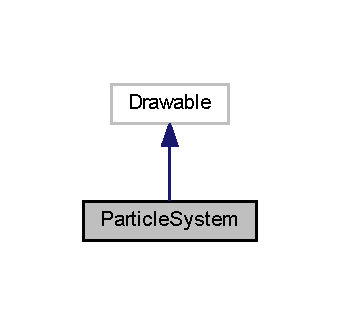
\includegraphics[width=163pt]{class_particle_system__inherit__graph}
\end{center}
\end{figure}


Collaboration diagram for Particle\+System\+:\nopagebreak
\begin{figure}[H]
\begin{center}
\leavevmode
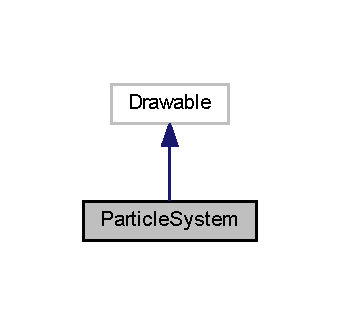
\includegraphics[width=163pt]{class_particle_system__coll__graph}
\end{center}
\end{figure}
\subsection*{Public Member Functions}
\begin{DoxyCompactItemize}
\item 
\mbox{\Hypertarget{class_particle_system_a9028ec8023c61773dd4a668c3ad8cc26}\label{class_particle_system_a9028ec8023c61773dd4a668c3ad8cc26}} 
\hyperlink{class_particle_system_a9028ec8023c61773dd4a668c3ad8cc26}{Particle\+System} ()
\begin{DoxyCompactList}\small\item\em Default constructor. \end{DoxyCompactList}\item 
\mbox{\Hypertarget{class_particle_system_a6bc725349a763b9d6817950cde16a93f}\label{class_particle_system_a6bc725349a763b9d6817950cde16a93f}} 
\hyperlink{class_particle_system_a6bc725349a763b9d6817950cde16a93f}{$\sim$\+Particle\+System} ()
\begin{DoxyCompactList}\small\item\em Destructor. \end{DoxyCompactList}\item 
void \hyperlink{class_particle_system_a448310d2188470d1a95d41d88bfb802a}{Explosion} (sf\+::\+Vector2f p\+\_\+\+Position, sf\+::\+Vector2f p\+\_\+\+Acceleration, float p\+\_\+\+Max\+Initial\+Speed, unsigned int p\+\_\+\+Amount, float p\+\_\+\+Life\+Time, float p\+\_\+\+Restitution, float p\+\_\+\+Density, float p\+\_\+\+Drag\+Co)
\item 
void \hyperlink{class_particle_system_aee020d9307645eca7af65287f196d9c2}{Update} (float p\+\_\+\+Delta\+Time)
\item 
\hyperlink{class_particle}{Particle} \& \hyperlink{class_particle_system_a0b5140b76ebaa019c073e1eabb07ab4f}{get\+Particle} (unsigned int p\+\_\+\+Index)
\item 
\mbox{\Hypertarget{class_particle_system_a1cb803dde4eb9c586aafffb7bdad65c9}\label{class_particle_system_a1cb803dde4eb9c586aafffb7bdad65c9}} 
unsigned int \hyperlink{class_particle_system_a1cb803dde4eb9c586aafffb7bdad65c9}{size} ()
\begin{DoxyCompactList}\small\item\em returns the amount of particles \end{DoxyCompactList}\item 
void \hyperlink{class_particle_system_aae99e6864b2dec1343ad6e01d33dd5a1}{draw} (sf\+::\+Render\+Target \&target, sf\+::\+Render\+States states) const
\end{DoxyCompactItemize}


\subsection{Detailed Description}
A class that handles updating particles and drawing their respective vertices. 

\subsection{Member Function Documentation}
\mbox{\Hypertarget{class_particle_system_aae99e6864b2dec1343ad6e01d33dd5a1}\label{class_particle_system_aae99e6864b2dec1343ad6e01d33dd5a1}} 
\index{Particle\+System@{Particle\+System}!draw@{draw}}
\index{draw@{draw}!Particle\+System@{Particle\+System}}
\subsubsection{\texorpdfstring{draw()}{draw()}}
{\footnotesize\ttfamily void Particle\+System\+::draw (\begin{DoxyParamCaption}\item[{sf\+::\+Render\+Target \&}]{target,  }\item[{sf\+::\+Render\+States}]{states }\end{DoxyParamCaption}) const}

Draw 
\begin{DoxyParams}[1]{Parameters}
\mbox{\tt in,out}  & {\em target} & Render target to draw to \\
\hline
\mbox{\tt in}  & {\em states} & Render state \\
\hline
\end{DoxyParams}
\mbox{\Hypertarget{class_particle_system_a448310d2188470d1a95d41d88bfb802a}\label{class_particle_system_a448310d2188470d1a95d41d88bfb802a}} 
\index{Particle\+System@{Particle\+System}!Explosion@{Explosion}}
\index{Explosion@{Explosion}!Particle\+System@{Particle\+System}}
\subsubsection{\texorpdfstring{Explosion()}{Explosion()}}
{\footnotesize\ttfamily void Particle\+System\+::\+Explosion (\begin{DoxyParamCaption}\item[{sf\+::\+Vector2f}]{p\+\_\+\+Position,  }\item[{sf\+::\+Vector2f}]{p\+\_\+\+Acceleration,  }\item[{float}]{p\+\_\+\+Max\+Initial\+Speed,  }\item[{unsigned int}]{p\+\_\+\+Amount,  }\item[{float}]{p\+\_\+\+Life\+Time,  }\item[{float}]{p\+\_\+\+Restitution,  }\item[{float}]{p\+\_\+\+Density,  }\item[{float}]{p\+\_\+\+Drag\+Co }\end{DoxyParamCaption})}

Creates an explosions of particles 
\begin{DoxyParams}[1]{Parameters}
\mbox{\tt in}  & {\em p\+\_\+\+Position} & Initial Position \\
\hline
\mbox{\tt in}  & {\em p\+\_\+\+Acceleration} & Intial Acceleration \\
\hline
\mbox{\tt in}  & {\em p\+\_\+\+Max\+Initial\+Speed} & Maximum possible speed of a particle \\
\hline
\mbox{\tt in}  & {\em p\+\_\+\+Amount} & Amount of particles to spawn \\
\hline
\mbox{\tt in}  & {\em p\+\_\+\+Life\+Time} & Time before a particle despawns \\
\hline
\mbox{\tt in}  & {\em p\+\_\+\+Restitution} & Initial restitution \\
\hline
\mbox{\tt in}  & {\em p\+\_\+\+Density} & Initial density \\
\hline
\mbox{\tt in}  & {\em p\+\_\+\+Drag\+Co} & Initial drag coefficient \\
\hline
\end{DoxyParams}
\mbox{\Hypertarget{class_particle_system_a0b5140b76ebaa019c073e1eabb07ab4f}\label{class_particle_system_a0b5140b76ebaa019c073e1eabb07ab4f}} 
\index{Particle\+System@{Particle\+System}!get\+Particle@{get\+Particle}}
\index{get\+Particle@{get\+Particle}!Particle\+System@{Particle\+System}}
\subsubsection{\texorpdfstring{get\+Particle()}{getParticle()}}
{\footnotesize\ttfamily \hyperlink{class_particle}{Particle}\& Particle\+System\+::get\+Particle (\begin{DoxyParamCaption}\item[{unsigned int}]{p\+\_\+\+Index }\end{DoxyParamCaption})}

returns a reference to a particle 
\begin{DoxyParams}[1]{Parameters}
\mbox{\tt in}  & {\em p\+\_\+\+Index} & The index of the particle you want to get \\
\hline
\end{DoxyParams}
\mbox{\Hypertarget{class_particle_system_aee020d9307645eca7af65287f196d9c2}\label{class_particle_system_aee020d9307645eca7af65287f196d9c2}} 
\index{Particle\+System@{Particle\+System}!Update@{Update}}
\index{Update@{Update}!Particle\+System@{Particle\+System}}
\subsubsection{\texorpdfstring{Update()}{Update()}}
{\footnotesize\ttfamily void Particle\+System\+::\+Update (\begin{DoxyParamCaption}\item[{float}]{p\+\_\+\+Delta\+Time }\end{DoxyParamCaption})}

Update the particles and vertex positions 
\begin{DoxyParams}[1]{Parameters}
\mbox{\tt in}  & {\em p\+\_\+\+Delta\+Time} & time elapsed since last frame \\
\hline
\end{DoxyParams}


The documentation for this class was generated from the following file\+:\begin{DoxyCompactItemize}
\item 
include/\hyperlink{_particle_system_8h}{Particle\+System.\+h}\end{DoxyCompactItemize}

\hypertarget{class_projectile}{}\section{Projectile Class Reference}
\label{class_projectile}\index{Projectile@{Projectile}}


A dynamic object that has damage.  




{\ttfamily \#include $<$Projectile.\+h$>$}



Inheritance diagram for Projectile\+:\nopagebreak
\begin{figure}[H]
\begin{center}
\leavevmode
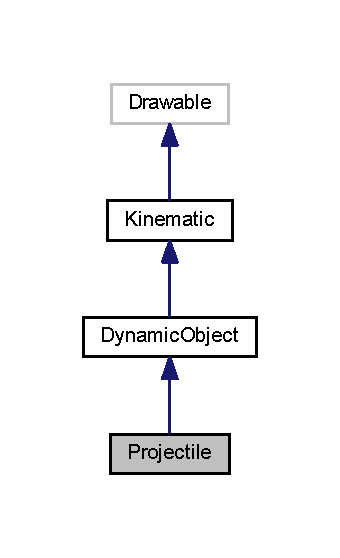
\includegraphics[width=163pt]{class_projectile__inherit__graph}
\end{center}
\end{figure}


Collaboration diagram for Projectile\+:\nopagebreak
\begin{figure}[H]
\begin{center}
\leavevmode
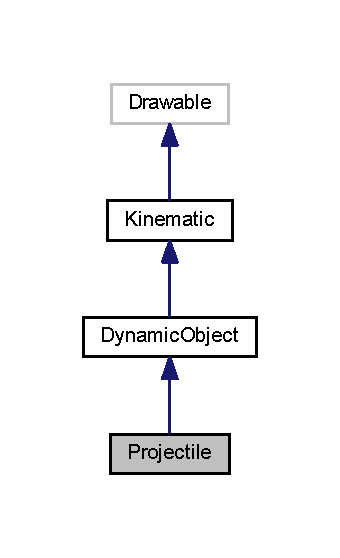
\includegraphics[width=163pt]{class_projectile__coll__graph}
\end{center}
\end{figure}
\subsection*{Public Member Functions}
\begin{DoxyCompactItemize}
\item 
\hyperlink{class_projectile_a5ed941ee600a7455a2c91fbacec4857e}{Projectile} (sf\+::\+Texture $\ast$p\+\_\+\+Texture, float p\+\_\+\+Restitution, sf\+::\+Vector2f p\+\_\+\+Size, sf\+::\+Vector2f p\+\_\+\+Start\+Pos, float p\+\_\+\+Density, float p\+\_\+\+Drag\+Co, float p\+\_\+\+Fric\+Co, float p\+\_\+\+Damage)
\item 
\mbox{\Hypertarget{class_projectile_a94903e021fa2edab60ba3836ca0b937d}\label{class_projectile_a94903e021fa2edab60ba3836ca0b937d}} 
\hyperlink{class_projectile_a94903e021fa2edab60ba3836ca0b937d}{$\sim$\+Projectile} ()
\begin{DoxyCompactList}\small\item\em Destructor. \end{DoxyCompactList}\item 
\mbox{\Hypertarget{class_projectile_a69b205e012801b3b7b146790ededd8d6}\label{class_projectile_a69b205e012801b3b7b146790ededd8d6}} 
float \hyperlink{class_projectile_a69b205e012801b3b7b146790ededd8d6}{area} ()
\begin{DoxyCompactList}\small\item\em Return area. \end{DoxyCompactList}\item 
\mbox{\Hypertarget{class_projectile_aad46fba4622a73c53b933486e60bf841}\label{class_projectile_aad46fba4622a73c53b933486e60bf841}} 
float \hyperlink{class_projectile_aad46fba4622a73c53b933486e60bf841}{get\+Damage} ()
\begin{DoxyCompactList}\small\item\em Get damage value. \end{DoxyCompactList}\item 
void \hyperlink{class_projectile_ac61792f1670310d35ecec906ab5ada9d}{draw} (sf\+::\+Render\+Target \&target, sf\+::\+Render\+States states) const
\end{DoxyCompactItemize}
\subsection*{Protected Attributes}
\begin{DoxyCompactItemize}
\item 
\mbox{\Hypertarget{class_projectile_a96e6a3198e2a1561ff4b7eaa3e19a378}\label{class_projectile_a96e6a3198e2a1561ff4b7eaa3e19a378}} 
sf\+::\+Sprite \hyperlink{class_projectile_a96e6a3198e2a1561ff4b7eaa3e19a378}{m\+\_\+\+Sprite}
\begin{DoxyCompactList}\small\item\em Sprite to draw projectile texture. \end{DoxyCompactList}\item 
\mbox{\Hypertarget{class_projectile_ada5ceb970f091739251d7ae10b94d159}\label{class_projectile_ada5ceb970f091739251d7ae10b94d159}} 
float \hyperlink{class_projectile_ada5ceb970f091739251d7ae10b94d159}{m\+\_\+\+Damage}
\begin{DoxyCompactList}\small\item\em Damage value. \end{DoxyCompactList}\end{DoxyCompactItemize}
\subsection*{Additional Inherited Members}


\subsection{Detailed Description}
A dynamic object that has damage. 

\subsection{Constructor \& Destructor Documentation}
\mbox{\Hypertarget{class_projectile_a5ed941ee600a7455a2c91fbacec4857e}\label{class_projectile_a5ed941ee600a7455a2c91fbacec4857e}} 
\index{Projectile@{Projectile}!Projectile@{Projectile}}
\index{Projectile@{Projectile}!Projectile@{Projectile}}
\subsubsection{\texorpdfstring{Projectile()}{Projectile()}}
{\footnotesize\ttfamily Projectile\+::\+Projectile (\begin{DoxyParamCaption}\item[{sf\+::\+Texture $\ast$}]{p\+\_\+\+Texture,  }\item[{float}]{p\+\_\+\+Restitution,  }\item[{sf\+::\+Vector2f}]{p\+\_\+\+Size,  }\item[{sf\+::\+Vector2f}]{p\+\_\+\+Start\+Pos,  }\item[{float}]{p\+\_\+\+Density,  }\item[{float}]{p\+\_\+\+Drag\+Co,  }\item[{float}]{p\+\_\+\+Fric\+Co,  }\item[{float}]{p\+\_\+\+Damage }\end{DoxyParamCaption})}

Constructor 
\begin{DoxyParams}[1]{Parameters}
\mbox{\tt in}  & {\em p\+\_\+\+Texture} & Initial texture \\
\hline
\mbox{\tt in}  & {\em p\+\_\+\+Restitution} & Intial bounciness \\
\hline
\mbox{\tt in}  & {\em p\+\_\+\+Size} & Initial size of the the axis aligned bounding box \\
\hline
\mbox{\tt in}  & {\em p\+\_\+\+Start\+Pos} & Initial position of the rocket \\
\hline
\mbox{\tt in}  & {\em p\+\_\+\+Density} & Initial density \\
\hline
\mbox{\tt in}  & {\em p\+\_\+\+Drag\+Co} & Intial drag coefficient \\
\hline
\mbox{\tt in}  & {\em p\+\_\+\+Fric\+Co} & Intial friction coefficient \\
\hline
\mbox{\tt in}  & {\em p\+\_\+\+Damage} & Initial damage value \\
\hline
\end{DoxyParams}


\subsection{Member Function Documentation}
\mbox{\Hypertarget{class_projectile_ac61792f1670310d35ecec906ab5ada9d}\label{class_projectile_ac61792f1670310d35ecec906ab5ada9d}} 
\index{Projectile@{Projectile}!draw@{draw}}
\index{draw@{draw}!Projectile@{Projectile}}
\subsubsection{\texorpdfstring{draw()}{draw()}}
{\footnotesize\ttfamily void Projectile\+::draw (\begin{DoxyParamCaption}\item[{sf\+::\+Render\+Target \&}]{target,  }\item[{sf\+::\+Render\+States}]{states }\end{DoxyParamCaption}) const\hspace{0.3cm}{\ttfamily [virtual]}}

Draw 
\begin{DoxyParams}[1]{Parameters}
\mbox{\tt in,out}  & {\em target} & Render target to draw to \\
\hline
\mbox{\tt in}  & {\em states} & Render state \\
\hline
\end{DoxyParams}


Implements \hyperlink{class_kinematic_a5d403bfe970efc1f0cebc872e3e2898b}{Kinematic}.



The documentation for this class was generated from the following file\+:\begin{DoxyCompactItemize}
\item 
include/\hyperlink{_projectile_8h}{Projectile.\+h}\end{DoxyCompactItemize}

\hypertarget{class_random}{}\section{Random Class Reference}
\label{class_random}\index{Random@{Random}}


Singleton class that holds random number engines.  




{\ttfamily \#include $<$Random.\+h$>$}

\subsection*{Public Member Functions}
\begin{DoxyCompactItemize}
\item 
float \hyperlink{class_random_a00363b48c0e54b490a11957a40200bad}{get\+Rand} (float p\+\_\+\+Min, float p\+\_\+\+Max)
\item 
\mbox{\Hypertarget{class_random_a649b59f8ec026bdc1ec5aab2d8d5f98e}\label{class_random_a649b59f8ec026bdc1ec5aab2d8d5f98e}} 
\hyperlink{class_random_a649b59f8ec026bdc1ec5aab2d8d5f98e}{Random} (\hyperlink{class_random}{Random} const \&)=delete
\begin{DoxyCompactList}\small\item\em prevents the creation of multiple texture loaders \end{DoxyCompactList}\item 
\mbox{\Hypertarget{class_random_a1ba4b35433055f747ac97d847d39d7a4}\label{class_random_a1ba4b35433055f747ac97d847d39d7a4}} 
\hyperlink{class_random}{Random} \& \hyperlink{class_random_a1ba4b35433055f747ac97d847d39d7a4}{operator=} (\hyperlink{class_random}{Random} const \&)=delete
\begin{DoxyCompactList}\small\item\em prevents the creation of multiple texture loaders \end{DoxyCompactList}\end{DoxyCompactItemize}
\subsection*{Static Public Member Functions}
\begin{DoxyCompactItemize}
\item 
\mbox{\Hypertarget{class_random_a562d087178f9a4d17c5c034561774797}\label{class_random_a562d087178f9a4d17c5c034561774797}} 
static \hyperlink{class_random}{Random} $\ast$ \hyperlink{class_random_a562d087178f9a4d17c5c034561774797}{instance} ()
\begin{DoxyCompactList}\small\item\em Returns a pointer to the static texture loader. \end{DoxyCompactList}\end{DoxyCompactItemize}


\subsection{Detailed Description}
Singleton class that holds random number engines. 

\subsection{Member Function Documentation}
\mbox{\Hypertarget{class_random_a00363b48c0e54b490a11957a40200bad}\label{class_random_a00363b48c0e54b490a11957a40200bad}} 
\index{Random@{Random}!get\+Rand@{get\+Rand}}
\index{get\+Rand@{get\+Rand}!Random@{Random}}
\subsubsection{\texorpdfstring{get\+Rand()}{getRand()}}
{\footnotesize\ttfamily float Random\+::get\+Rand (\begin{DoxyParamCaption}\item[{float}]{p\+\_\+\+Min,  }\item[{float}]{p\+\_\+\+Max }\end{DoxyParamCaption})}

Get random number between a min and max inclusive 
\begin{DoxyParams}[1]{Parameters}
\mbox{\tt in}  & {\em p\+\_\+\+Min} & Minimum value \\
\hline
\mbox{\tt in}  & {\em p\+\_\+\+Max} & Maximum value \\
\hline
\end{DoxyParams}


The documentation for this class was generated from the following file\+:\begin{DoxyCompactItemize}
\item 
include/\hyperlink{_random_8h}{Random.\+h}\end{DoxyCompactItemize}

\hypertarget{class_rocket}{}\section{Rocket Class Reference}
\label{class_rocket}\index{Rocket@{Rocket}}


A playable rocket class that keeps track of fuel and life.  




{\ttfamily \#include $<$Rocket.\+h$>$}



Inheritance diagram for Rocket\+:\nopagebreak
\begin{figure}[H]
\begin{center}
\leavevmode
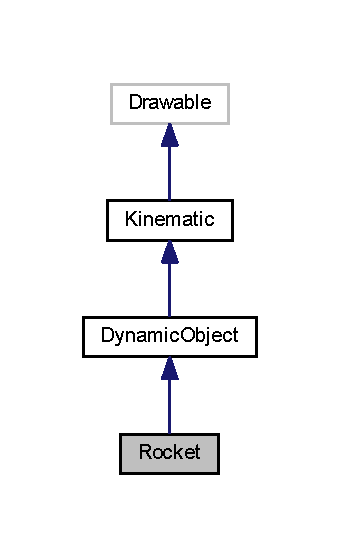
\includegraphics[width=163pt]{class_rocket__inherit__graph}
\end{center}
\end{figure}


Collaboration diagram for Rocket\+:\nopagebreak
\begin{figure}[H]
\begin{center}
\leavevmode
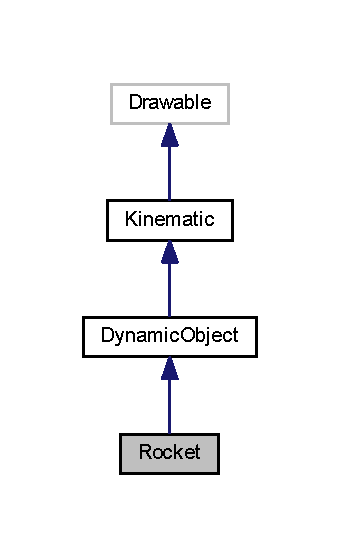
\includegraphics[width=163pt]{class_rocket__coll__graph}
\end{center}
\end{figure}
\subsection*{Public Member Functions}
\begin{DoxyCompactItemize}
\item 
\hyperlink{class_rocket_a5ddbd398e8bfa09b242d77d866651702}{Rocket} (sf\+::\+Texture $\ast$p\+\_\+\+Texture, float p\+\_\+\+Restitution, sf\+::\+Vector2f p\+\_\+\+Size, sf\+::\+Vector2f p\+\_\+\+Start\+Pos, float p\+\_\+\+Density, float p\+\_\+\+Drag\+Co, float p\+\_\+\+Fric\+Co, int p\+\_\+\+Team)
\item 
\mbox{\Hypertarget{class_rocket_ab0cbe044146250c3e592832bb4909ff9}\label{class_rocket_ab0cbe044146250c3e592832bb4909ff9}} 
\hyperlink{class_rocket_ab0cbe044146250c3e592832bb4909ff9}{$\sim$\+Rocket} ()
\begin{DoxyCompactList}\small\item\em Destructor. \end{DoxyCompactList}\item 
void \hyperlink{class_rocket_a3ecac400b4edb82d8288be25f9a0b949}{set\+Texture} (sf\+::\+Texture $\ast$p\+\_\+\+Texture)
\item 
void \hyperlink{class_rocket_a775dd0b77b6f82010d9ff201d266bf89}{set\+Life} (float p\+\_\+\+Life)
\item 
\mbox{\Hypertarget{class_rocket_ab6320ec0717a04f1709d91fb92d7cf74}\label{class_rocket_ab6320ec0717a04f1709d91fb92d7cf74}} 
float \hyperlink{class_rocket_ab6320ec0717a04f1709d91fb92d7cf74}{get\+Life} ()
\begin{DoxyCompactList}\small\item\em get life \end{DoxyCompactList}\item 
void \hyperlink{class_rocket_aac617e928cc99125cf014ac5dbb57b9b}{set\+Fuel} (float p\+\_\+\+Fuel)
\item 
\mbox{\Hypertarget{class_rocket_ad5e168da70869f966ddd535b38c18c8f}\label{class_rocket_ad5e168da70869f966ddd535b38c18c8f}} 
float \hyperlink{class_rocket_ad5e168da70869f966ddd535b38c18c8f}{get\+Fuel} ()
\begin{DoxyCompactList}\small\item\em get fuel \end{DoxyCompactList}\item 
\mbox{\Hypertarget{class_rocket_a43995d3f49c3d00f8d6c5bbe7aefc5e2}\label{class_rocket_a43995d3f49c3d00f8d6c5bbe7aefc5e2}} 
int \hyperlink{class_rocket_a43995d3f49c3d00f8d6c5bbe7aefc5e2}{get\+Team} ()
\begin{DoxyCompactList}\small\item\em get team \end{DoxyCompactList}\item 
\mbox{\Hypertarget{class_rocket_ad7c2bc69fc216ecb9320a77c044fff07}\label{class_rocket_ad7c2bc69fc216ecb9320a77c044fff07}} 
float \hyperlink{class_rocket_ad7c2bc69fc216ecb9320a77c044fff07}{area} ()
\begin{DoxyCompactList}\small\item\em returns the area \end{DoxyCompactList}\item 
void \hyperlink{class_rocket_a4b83a058408ee42ea77248dd8f0d3339}{draw} (sf\+::\+Render\+Target \&target, sf\+::\+Render\+States states) const
\end{DoxyCompactItemize}
\subsection*{Protected Attributes}
\begin{DoxyCompactItemize}
\item 
\mbox{\Hypertarget{class_rocket_a584dfdd155f46944168ebfd23b158bf2}\label{class_rocket_a584dfdd155f46944168ebfd23b158bf2}} 
sf\+::\+Sprite \hyperlink{class_rocket_a584dfdd155f46944168ebfd23b158bf2}{m\+\_\+\+Sprite}
\begin{DoxyCompactList}\small\item\em Sprite to draw rocket texture. \end{DoxyCompactList}\item 
\mbox{\Hypertarget{class_rocket_a5d12b42180029361f37e9ce86a75f1eb}\label{class_rocket_a5d12b42180029361f37e9ce86a75f1eb}} 
int \hyperlink{class_rocket_a5d12b42180029361f37e9ce86a75f1eb}{m\+\_\+\+Team} = 0
\begin{DoxyCompactList}\small\item\em Team value. \end{DoxyCompactList}\item 
\mbox{\Hypertarget{class_rocket_a6e8e5f6f965fa1fc8d7919b4c7a7d42b}\label{class_rocket_a6e8e5f6f965fa1fc8d7919b4c7a7d42b}} 
float \hyperlink{class_rocket_a6e8e5f6f965fa1fc8d7919b4c7a7d42b}{m\+\_\+\+Max\+Life} = 100.\+0f
\begin{DoxyCompactList}\small\item\em Maximum life. \end{DoxyCompactList}\item 
\mbox{\Hypertarget{class_rocket_a564ba8da5fdab5a6bccef0adfb58864d}\label{class_rocket_a564ba8da5fdab5a6bccef0adfb58864d}} 
float \hyperlink{class_rocket_a564ba8da5fdab5a6bccef0adfb58864d}{m\+\_\+\+Life} = 0.\+0f
\begin{DoxyCompactList}\small\item\em Current life. \end{DoxyCompactList}\item 
\mbox{\Hypertarget{class_rocket_a66c5adff518ec4cd545a3a669e8448c7}\label{class_rocket_a66c5adff518ec4cd545a3a669e8448c7}} 
float \hyperlink{class_rocket_a66c5adff518ec4cd545a3a669e8448c7}{m\+\_\+\+Life\+Bar\+Max\+Length}
\begin{DoxyCompactList}\small\item\em Life bar\textquotesingle{}s max length. \end{DoxyCompactList}\item 
\mbox{\Hypertarget{class_rocket_a8ae0960136c6fb41a9795ca555c1f61d}\label{class_rocket_a8ae0960136c6fb41a9795ca555c1f61d}} 
sf\+::\+Rectangle\+Shape \hyperlink{class_rocket_a8ae0960136c6fb41a9795ca555c1f61d}{m\+\_\+\+Life\+Bar}
\begin{DoxyCompactList}\small\item\em Life bar rectangle. \end{DoxyCompactList}\item 
\mbox{\Hypertarget{class_rocket_a931d317896687553b03709b1532ef00f}\label{class_rocket_a931d317896687553b03709b1532ef00f}} 
sf\+::\+Vector2f \hyperlink{class_rocket_a931d317896687553b03709b1532ef00f}{m\+\_\+\+Life\+Bar\+Offset}
\begin{DoxyCompactList}\small\item\em Life bar Offset from the rocket position. \end{DoxyCompactList}\item 
\mbox{\Hypertarget{class_rocket_ac27158eb4ce58650f76a258bef38bb8e}\label{class_rocket_ac27158eb4ce58650f76a258bef38bb8e}} 
float \hyperlink{class_rocket_ac27158eb4ce58650f76a258bef38bb8e}{m\+\_\+\+Max\+Fuel} = 250.\+0f
\begin{DoxyCompactList}\small\item\em Maximum fuel. \end{DoxyCompactList}\item 
\mbox{\Hypertarget{class_rocket_ab8321d9115c93fca3556d06d96edd627}\label{class_rocket_ab8321d9115c93fca3556d06d96edd627}} 
float \hyperlink{class_rocket_ab8321d9115c93fca3556d06d96edd627}{m\+\_\+\+Fuel} = 0.\+0f
\begin{DoxyCompactList}\small\item\em Current fuel. \end{DoxyCompactList}\item 
\mbox{\Hypertarget{class_rocket_ab2987e91884c522731200e5b4b3b53c2}\label{class_rocket_ab2987e91884c522731200e5b4b3b53c2}} 
float \hyperlink{class_rocket_ab2987e91884c522731200e5b4b3b53c2}{m\+\_\+\+Fuel\+Bar\+Max\+Length}
\begin{DoxyCompactList}\small\item\em Fuel bar\textquotesingle{}s max length. \end{DoxyCompactList}\item 
\mbox{\Hypertarget{class_rocket_a8db4d19c2b34f322d5d772bd39227c9c}\label{class_rocket_a8db4d19c2b34f322d5d772bd39227c9c}} 
sf\+::\+Rectangle\+Shape \hyperlink{class_rocket_a8db4d19c2b34f322d5d772bd39227c9c}{m\+\_\+\+Fuel\+Bar}
\begin{DoxyCompactList}\small\item\em Fuel bar\textquotesingle{}s rectangle. \end{DoxyCompactList}\item 
\mbox{\Hypertarget{class_rocket_ab490e90b430de879b899d572d9e84a4d}\label{class_rocket_ab490e90b430de879b899d572d9e84a4d}} 
sf\+::\+Vector2f \hyperlink{class_rocket_ab490e90b430de879b899d572d9e84a4d}{m\+\_\+\+Fuel\+Bar\+Offset}
\begin{DoxyCompactList}\small\item\em Fuel bar offset from rocket position. \end{DoxyCompactList}\end{DoxyCompactItemize}
\subsection*{Additional Inherited Members}


\subsection{Detailed Description}
A playable rocket class that keeps track of fuel and life. 

\subsection{Constructor \& Destructor Documentation}
\mbox{\Hypertarget{class_rocket_a5ddbd398e8bfa09b242d77d866651702}\label{class_rocket_a5ddbd398e8bfa09b242d77d866651702}} 
\index{Rocket@{Rocket}!Rocket@{Rocket}}
\index{Rocket@{Rocket}!Rocket@{Rocket}}
\subsubsection{\texorpdfstring{Rocket()}{Rocket()}}
{\footnotesize\ttfamily Rocket\+::\+Rocket (\begin{DoxyParamCaption}\item[{sf\+::\+Texture $\ast$}]{p\+\_\+\+Texture,  }\item[{float}]{p\+\_\+\+Restitution,  }\item[{sf\+::\+Vector2f}]{p\+\_\+\+Size,  }\item[{sf\+::\+Vector2f}]{p\+\_\+\+Start\+Pos,  }\item[{float}]{p\+\_\+\+Density,  }\item[{float}]{p\+\_\+\+Drag\+Co,  }\item[{float}]{p\+\_\+\+Fric\+Co,  }\item[{int}]{p\+\_\+\+Team }\end{DoxyParamCaption})}

Constructor 
\begin{DoxyParams}[1]{Parameters}
\mbox{\tt in}  & {\em p\+\_\+\+Texture} & Initial texture \\
\hline
\mbox{\tt in}  & {\em p\+\_\+\+Restitution} & Intial bounciness \\
\hline
\mbox{\tt in}  & {\em p\+\_\+\+Size} & Initial size of the the axis aligned bounding box \\
\hline
\mbox{\tt in}  & {\em p\+\_\+\+Start\+Pos} & Initial position of the rocket \\
\hline
\mbox{\tt in}  & {\em p\+\_\+\+Density} & Initial density \\
\hline
\mbox{\tt in}  & {\em p\+\_\+\+Drag\+Co} & Intial drag coefficient \\
\hline
\mbox{\tt in}  & {\em p\+\_\+\+Fric\+Co} & Intial friction coefficient \\
\hline
\mbox{\tt in}  & {\em p\+\_\+\+Team} & Initial team \\
\hline
\end{DoxyParams}


\subsection{Member Function Documentation}
\mbox{\Hypertarget{class_rocket_a4b83a058408ee42ea77248dd8f0d3339}\label{class_rocket_a4b83a058408ee42ea77248dd8f0d3339}} 
\index{Rocket@{Rocket}!draw@{draw}}
\index{draw@{draw}!Rocket@{Rocket}}
\subsubsection{\texorpdfstring{draw()}{draw()}}
{\footnotesize\ttfamily void Rocket\+::draw (\begin{DoxyParamCaption}\item[{sf\+::\+Render\+Target \&}]{target,  }\item[{sf\+::\+Render\+States}]{states }\end{DoxyParamCaption}) const\hspace{0.3cm}{\ttfamily [virtual]}}

Draw 
\begin{DoxyParams}[1]{Parameters}
\mbox{\tt in,out}  & {\em target} & Render target to draw to \\
\hline
\mbox{\tt in}  & {\em states} & Render state \\
\hline
\end{DoxyParams}


Implements \hyperlink{class_kinematic_a5d403bfe970efc1f0cebc872e3e2898b}{Kinematic}.

\mbox{\Hypertarget{class_rocket_aac617e928cc99125cf014ac5dbb57b9b}\label{class_rocket_aac617e928cc99125cf014ac5dbb57b9b}} 
\index{Rocket@{Rocket}!set\+Fuel@{set\+Fuel}}
\index{set\+Fuel@{set\+Fuel}!Rocket@{Rocket}}
\subsubsection{\texorpdfstring{set\+Fuel()}{setFuel()}}
{\footnotesize\ttfamily void Rocket\+::set\+Fuel (\begin{DoxyParamCaption}\item[{float}]{p\+\_\+\+Fuel }\end{DoxyParamCaption})}

set the fuel 
\begin{DoxyParams}[1]{Parameters}
\mbox{\tt in}  & {\em p\+\_\+\+Fuel} & fuel value \\
\hline
\end{DoxyParams}
\mbox{\Hypertarget{class_rocket_a775dd0b77b6f82010d9ff201d266bf89}\label{class_rocket_a775dd0b77b6f82010d9ff201d266bf89}} 
\index{Rocket@{Rocket}!set\+Life@{set\+Life}}
\index{set\+Life@{set\+Life}!Rocket@{Rocket}}
\subsubsection{\texorpdfstring{set\+Life()}{setLife()}}
{\footnotesize\ttfamily void Rocket\+::set\+Life (\begin{DoxyParamCaption}\item[{float}]{p\+\_\+\+Life }\end{DoxyParamCaption})}

Set the life 
\begin{DoxyParams}[1]{Parameters}
\mbox{\tt in}  & {\em p\+\_\+\+Life} & life value \\
\hline
\end{DoxyParams}
\mbox{\Hypertarget{class_rocket_a3ecac400b4edb82d8288be25f9a0b949}\label{class_rocket_a3ecac400b4edb82d8288be25f9a0b949}} 
\index{Rocket@{Rocket}!set\+Texture@{set\+Texture}}
\index{set\+Texture@{set\+Texture}!Rocket@{Rocket}}
\subsubsection{\texorpdfstring{set\+Texture()}{setTexture()}}
{\footnotesize\ttfamily void Rocket\+::set\+Texture (\begin{DoxyParamCaption}\item[{sf\+::\+Texture $\ast$}]{p\+\_\+\+Texture }\end{DoxyParamCaption})}

Set the texture 
\begin{DoxyParams}[1]{Parameters}
\mbox{\tt in}  & {\em p\+\_\+\+Texture} & Chosen texture to switch to \\
\hline
\end{DoxyParams}


The documentation for this class was generated from the following file\+:\begin{DoxyCompactItemize}
\item 
include/\hyperlink{_rocket_8h}{Rocket.\+h}\end{DoxyCompactItemize}

\hypertarget{class_scene}{}\section{Scene Class Reference}
\label{class_scene}\index{Scene@{Scene}}


A class that provides late binding methods for an interactable screen e.\+g. a game or a menu.  




{\ttfamily \#include $<$Scene.\+h$>$}



Inheritance diagram for Scene\+:\nopagebreak
\begin{figure}[H]
\begin{center}
\leavevmode
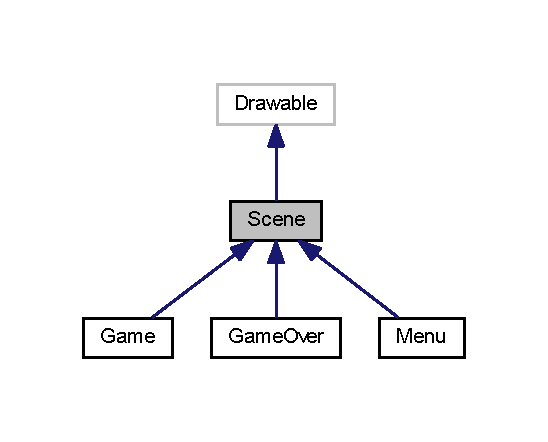
\includegraphics[width=263pt]{class_scene__inherit__graph}
\end{center}
\end{figure}


Collaboration diagram for Scene\+:\nopagebreak
\begin{figure}[H]
\begin{center}
\leavevmode
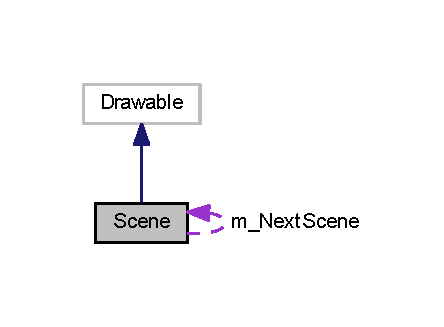
\includegraphics[width=213pt]{class_scene__coll__graph}
\end{center}
\end{figure}
\subsection*{Public Member Functions}
\begin{DoxyCompactItemize}
\item 
\mbox{\Hypertarget{class_scene_ad10176d75a9cc0da56626f682d083507}\label{class_scene_ad10176d75a9cc0da56626f682d083507}} 
\hyperlink{class_scene_ad10176d75a9cc0da56626f682d083507}{Scene} ()
\begin{DoxyCompactList}\small\item\em Default constructor. \end{DoxyCompactList}\item 
\mbox{\Hypertarget{class_scene_a3b8cec2e32546713915f8c6303c951f1}\label{class_scene_a3b8cec2e32546713915f8c6303c951f1}} 
\hyperlink{class_scene_a3b8cec2e32546713915f8c6303c951f1}{$\sim$\+Scene} ()
\begin{DoxyCompactList}\small\item\em Destructor. \end{DoxyCompactList}\item 
virtual void \hyperlink{class_scene_a182f90e2638c0da6a8ba2eab7cdc73ae}{handle\+Keyboard\+Input} (int p\+\_\+\+Key)=0
\item 
virtual void \hyperlink{class_scene_ad9240c92a58c4dba4c2409ec8bcff686}{handle\+Mouse\+Input} (sf\+::\+Mouse\+::\+Button p\+\_\+\+Button)=0
\item 
void \hyperlink{class_scene_a2cdbd23d08e1faa0becceaf8bd130ac7}{handle\+Mouse\+Move} (const sf\+::\+Render\+Window \&p\+\_\+\+Window)
\item 
virtual void \hyperlink{class_scene_a461d21cd952c7dd0556850a3fc95a760}{update} (float p\+\_\+\+Time\+Step)=0
\item 
virtual void \hyperlink{class_scene_ac3fd1d41fa7b7516eeff009de7550552}{draw} (sf\+::\+Render\+Target \&target, sf\+::\+Render\+States states) const =0
\item 
\mbox{\Hypertarget{class_scene_a6229a5c43e32fe5b92357e61850e8b0d}\label{class_scene_a6229a5c43e32fe5b92357e61850e8b0d}} 
\hyperlink{class_scene}{Scene} $\ast$ \hyperlink{class_scene_a6229a5c43e32fe5b92357e61850e8b0d}{get\+Next\+Scene} ()
\begin{DoxyCompactList}\small\item\em Returns a pointer to the heap for the next scene. \end{DoxyCompactList}\item 
\mbox{\Hypertarget{class_scene_a67993233347f2f6ab2765598b627d9aa}\label{class_scene_a67993233347f2f6ab2765598b627d9aa}} 
bool \hyperlink{class_scene_a67993233347f2f6ab2765598b627d9aa}{is\+Scene\+Finished} ()
\begin{DoxyCompactList}\small\item\em Returns true if m\+\_\+\+Next\+Scene isnt a nullptr. \end{DoxyCompactList}\item 
\mbox{\Hypertarget{class_scene_afb6e039ff2c88295876cf83e599644f4}\label{class_scene_afb6e039ff2c88295876cf83e599644f4}} 
bool \hyperlink{class_scene_afb6e039ff2c88295876cf83e599644f4}{get\+Debug} ()
\begin{DoxyCompactList}\small\item\em Returns the debug state. \end{DoxyCompactList}\end{DoxyCompactItemize}
\subsection*{Protected Attributes}
\begin{DoxyCompactItemize}
\item 
\mbox{\Hypertarget{class_scene_a7c893a2bcd5b45f758d1ca2596f2c080}\label{class_scene_a7c893a2bcd5b45f758d1ca2596f2c080}} 
bool \hyperlink{class_scene_a7c893a2bcd5b45f758d1ca2596f2c080}{m\+\_\+\+Debug} = false
\begin{DoxyCompactList}\small\item\em Debug boolean. \end{DoxyCompactList}\item 
\mbox{\Hypertarget{class_scene_ac481124f477d63e6c71993685b4bd675}\label{class_scene_ac481124f477d63e6c71993685b4bd675}} 
sf\+::\+View \hyperlink{class_scene_ac481124f477d63e6c71993685b4bd675}{m\+\_\+\+View}
\begin{DoxyCompactList}\small\item\em The view. \end{DoxyCompactList}\item 
\mbox{\Hypertarget{class_scene_a7f2cc1644a291a7102b8e1d069541d65}\label{class_scene_a7f2cc1644a291a7102b8e1d069541d65}} 
\hyperlink{class_scene}{Scene} $\ast$ \hyperlink{class_scene_a7f2cc1644a291a7102b8e1d069541d65}{m\+\_\+\+Next\+Scene} = nullptr
\begin{DoxyCompactList}\small\item\em Pointer to next scene. \end{DoxyCompactList}\item 
\mbox{\Hypertarget{class_scene_a2f342aba86b1baa65a92a201ebf89502}\label{class_scene_a2f342aba86b1baa65a92a201ebf89502}} 
sf\+::\+Vector2u \hyperlink{class_scene_a2f342aba86b1baa65a92a201ebf89502}{m\+\_\+\+Window\+Size}
\begin{DoxyCompactList}\small\item\em A copy of the initial window size. \end{DoxyCompactList}\item 
\mbox{\Hypertarget{class_scene_a4714ea68285b5fb621f9355ac09f3a63}\label{class_scene_a4714ea68285b5fb621f9355ac09f3a63}} 
sf\+::\+Vector2f \hyperlink{class_scene_a4714ea68285b5fb621f9355ac09f3a63}{m\+\_\+\+Mouse\+World\+Pos}
\begin{DoxyCompactList}\small\item\em The current mouse pos. \end{DoxyCompactList}\end{DoxyCompactItemize}


\subsection{Detailed Description}
A class that provides late binding methods for an interactable screen e.\+g. a game or a menu. 

\subsection{Member Function Documentation}
\mbox{\Hypertarget{class_scene_ac3fd1d41fa7b7516eeff009de7550552}\label{class_scene_ac3fd1d41fa7b7516eeff009de7550552}} 
\index{Scene@{Scene}!draw@{draw}}
\index{draw@{draw}!Scene@{Scene}}
\subsubsection{\texorpdfstring{draw()}{draw()}}
{\footnotesize\ttfamily virtual void Scene\+::draw (\begin{DoxyParamCaption}\item[{sf\+::\+Render\+Target \&}]{target,  }\item[{sf\+::\+Render\+States}]{states }\end{DoxyParamCaption}) const\hspace{0.3cm}{\ttfamily [pure virtual]}}

Draw 
\begin{DoxyParams}[1]{Parameters}
\mbox{\tt in,out}  & {\em target} & Render target to draw to \\
\hline
\mbox{\tt in}  & {\em states} & Render state \\
\hline
\end{DoxyParams}


Implemented in \hyperlink{class_game_a143d1a2f8a527db60f1fe47ab3d854a7}{Game}, \hyperlink{class_game_over_a4792ee9e2b587f98576a8023d34f5f5c}{Game\+Over}, and \hyperlink{class_menu_aa0e69963ee402f3559680e5a691b03fd}{Menu}.

\mbox{\Hypertarget{class_scene_a182f90e2638c0da6a8ba2eab7cdc73ae}\label{class_scene_a182f90e2638c0da6a8ba2eab7cdc73ae}} 
\index{Scene@{Scene}!handle\+Keyboard\+Input@{handle\+Keyboard\+Input}}
\index{handle\+Keyboard\+Input@{handle\+Keyboard\+Input}!Scene@{Scene}}
\subsubsection{\texorpdfstring{handle\+Keyboard\+Input()}{handleKeyboardInput()}}
{\footnotesize\ttfamily virtual void Scene\+::handle\+Keyboard\+Input (\begin{DoxyParamCaption}\item[{int}]{p\+\_\+\+Key }\end{DoxyParamCaption})\hspace{0.3cm}{\ttfamily [pure virtual]}}

Handle keyboard input events 
\begin{DoxyParams}[1]{Parameters}
\mbox{\tt in}  & {\em p\+\_\+\+Key} & The Key that was pressed \\
\hline
\end{DoxyParams}


Implemented in \hyperlink{class_game_a6ccc7e91593f06a0e722cc419016a237}{Game}, \hyperlink{class_game_over_aae04263371e8f82199df51de54ef77d1}{Game\+Over}, and \hyperlink{class_menu_a2ebc63a5e64b90dcfae4284e7f7f4be6}{Menu}.

\mbox{\Hypertarget{class_scene_ad9240c92a58c4dba4c2409ec8bcff686}\label{class_scene_ad9240c92a58c4dba4c2409ec8bcff686}} 
\index{Scene@{Scene}!handle\+Mouse\+Input@{handle\+Mouse\+Input}}
\index{handle\+Mouse\+Input@{handle\+Mouse\+Input}!Scene@{Scene}}
\subsubsection{\texorpdfstring{handle\+Mouse\+Input()}{handleMouseInput()}}
{\footnotesize\ttfamily virtual void Scene\+::handle\+Mouse\+Input (\begin{DoxyParamCaption}\item[{sf\+::\+Mouse\+::\+Button}]{p\+\_\+\+Button }\end{DoxyParamCaption})\hspace{0.3cm}{\ttfamily [pure virtual]}}

Handle mouse input events 
\begin{DoxyParams}[1]{Parameters}
\mbox{\tt in}  & {\em p\+\_\+\+Button} & The button that was pressed \\
\hline
\end{DoxyParams}


Implemented in \hyperlink{class_game_a1c0ddbb7a468997249acbdd6cf2dbe34}{Game}, \hyperlink{class_game_over_a83c0cecb3faab5ea8c36272e931006f7}{Game\+Over}, and \hyperlink{class_menu_a4f99fe96e47268bd4561df0c8faa23c8}{Menu}.

\mbox{\Hypertarget{class_scene_a2cdbd23d08e1faa0becceaf8bd130ac7}\label{class_scene_a2cdbd23d08e1faa0becceaf8bd130ac7}} 
\index{Scene@{Scene}!handle\+Mouse\+Move@{handle\+Mouse\+Move}}
\index{handle\+Mouse\+Move@{handle\+Mouse\+Move}!Scene@{Scene}}
\subsubsection{\texorpdfstring{handle\+Mouse\+Move()}{handleMouseMove()}}
{\footnotesize\ttfamily void Scene\+::handle\+Mouse\+Move (\begin{DoxyParamCaption}\item[{const sf\+::\+Render\+Window \&}]{p\+\_\+\+Window }\end{DoxyParamCaption})}

Handle mouse mouse movement 
\begin{DoxyParams}[1]{Parameters}
\mbox{\tt in}  & {\em p\+\_\+\+Window} & Used to calculate mouse pos relative to the window \\
\hline
\end{DoxyParams}
\mbox{\Hypertarget{class_scene_a461d21cd952c7dd0556850a3fc95a760}\label{class_scene_a461d21cd952c7dd0556850a3fc95a760}} 
\index{Scene@{Scene}!update@{update}}
\index{update@{update}!Scene@{Scene}}
\subsubsection{\texorpdfstring{update()}{update()}}
{\footnotesize\ttfamily virtual void Scene\+::update (\begin{DoxyParamCaption}\item[{float}]{p\+\_\+\+Time\+Step }\end{DoxyParamCaption})\hspace{0.3cm}{\ttfamily [pure virtual]}}

Update the scene 
\begin{DoxyParams}[1]{Parameters}
\mbox{\tt in}  & {\em p\+\_\+\+Time\+Step} & the change in time since the last frame \\
\hline
\end{DoxyParams}


Implemented in \hyperlink{class_game_a3fd12339411955db6a5445ba213ef293}{Game}, \hyperlink{class_game_over_a6b9465b5c095a1de0e467baf17045fac}{Game\+Over}, and \hyperlink{class_menu_a8043b25a060513367b0e286d3ae397d2}{Menu}.



The documentation for this class was generated from the following file\+:\begin{DoxyCompactItemize}
\item 
include/\hyperlink{_scene_8h}{Scene.\+h}\end{DoxyCompactItemize}

\hypertarget{class_terrain}{}\section{Terrain Class Reference}
\label{class_terrain}\index{Terrain@{Terrain}}
Inheritance diagram for Terrain\+:\begin{figure}[H]
\begin{center}
\leavevmode
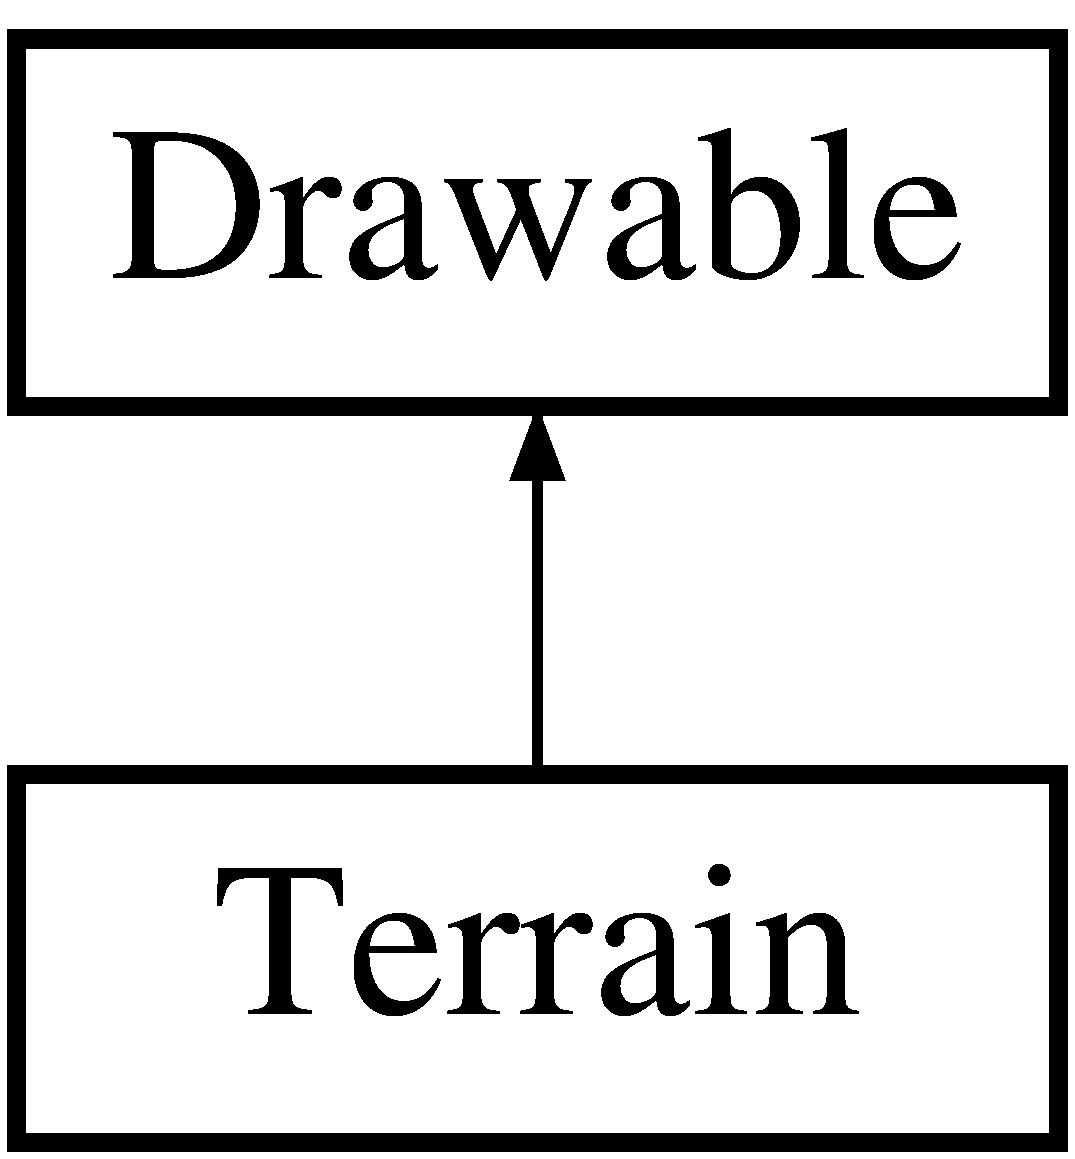
\includegraphics[height=2.000000cm]{class_terrain}
\end{center}
\end{figure}
\subsection*{Public Member Functions}
\begin{DoxyCompactItemize}
\item 
\mbox{\Hypertarget{class_terrain_ab42c4af61b057ccc1af4f2ebbfefa550}\label{class_terrain_ab42c4af61b057ccc1af4f2ebbfefa550}} 
void {\bfseries Load\+Terrain} (sf\+::\+Texture $\ast$p\+\_\+\+Texture)
\item 
\mbox{\Hypertarget{class_terrain_a728b4b72b41aaf1ed463652737b81b37}\label{class_terrain_a728b4b72b41aaf1ed463652737b81b37}} 
sf\+::\+Vector2f {\bfseries Get\+Normal} (unsigned int p\+\_\+X, unsigned int p\+\_\+Y, int p\+\_\+\+Radius)
\item 
\mbox{\Hypertarget{class_terrain_a1929db8af46f2b4a1a053ac33b495bb1}\label{class_terrain_a1929db8af46f2b4a1a053ac33b495bb1}} 
void {\bfseries Subtract\+Shape} (sf\+::\+Shape $\ast$p\+\_\+\+Shape)
\item 
\mbox{\Hypertarget{class_terrain_a46d26ac3525b10ca6bbf065b2627c2b6}\label{class_terrain_a46d26ac3525b10ca6bbf065b2627c2b6}} 
void {\bfseries draw} (sf\+::\+Render\+Target \&target, sf\+::\+Render\+States states) const
\end{DoxyCompactItemize}


The documentation for this class was generated from the following file\+:\begin{DoxyCompactItemize}
\item 
include/\hyperlink{_terrain_8h}{Terrain.\+h}\end{DoxyCompactItemize}

\hypertarget{class_text_button}{}\section{Text\+Button Class Reference}
\label{class_text_button}\index{Text\+Button@{Text\+Button}}


A Wrapper class for sf\+::\+Text and sf\+::\+Font that adds a mosue over checker.  




{\ttfamily \#include $<$Text\+Button.\+h$>$}



Inheritance diagram for Text\+Button\+:\nopagebreak
\begin{figure}[H]
\begin{center}
\leavevmode
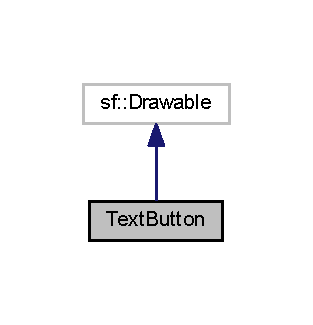
\includegraphics[width=150pt]{class_text_button__inherit__graph}
\end{center}
\end{figure}


Collaboration diagram for Text\+Button\+:\nopagebreak
\begin{figure}[H]
\begin{center}
\leavevmode
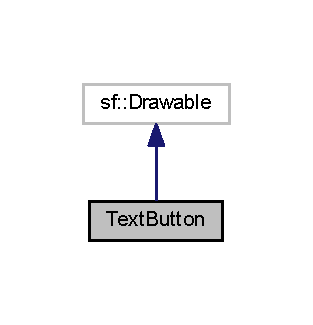
\includegraphics[width=150pt]{class_text_button__coll__graph}
\end{center}
\end{figure}
\subsection*{Public Member Functions}
\begin{DoxyCompactItemize}
\item 
\hyperlink{class_text_button_a03347de6b8c774f7a78a8ce6bbab10fc}{Text\+Button} (sf\+::\+Font p\+\_\+\+Font, std\+::string p\+\_\+\+String, float p\+\_\+\+Char\+Size, sf\+::\+Color p\+\_\+\+Base\+Color, sf\+::\+Color p\+\_\+\+Over\+Color)
\item 
\mbox{\Hypertarget{class_text_button_a497a17bb110e249c7eb88a98dad12192}\label{class_text_button_a497a17bb110e249c7eb88a98dad12192}} 
\hyperlink{class_text_button_a497a17bb110e249c7eb88a98dad12192}{$\sim$\+Text\+Button} ()
\begin{DoxyCompactList}\small\item\em Destructor. \end{DoxyCompactList}\item 
void \hyperlink{class_text_button_a8a9500a6a76540c73a15ff3a4ceca08a}{set\+Position} (sf\+::\+Vector2f p\+\_\+\+Position)
\item 
void \hyperlink{class_text_button_a255b855a91d7e488fa674abaf302edbb}{update} (sf\+::\+Vector2f p\+\_\+\+Mouse\+Pos)
\item 
bool \hyperlink{class_text_button_a10d99e4de442f5c2bb72ab6b9938813f}{is\+Mouse\+Over} (sf\+::\+Vector2f p\+\_\+\+Mouse\+Pos)
\item 
void \hyperlink{class_text_button_a8b52953d08ee55b437c97843628774c8}{draw} (sf\+::\+Render\+Target \&target, sf\+::\+Render\+States states) const
\end{DoxyCompactItemize}


\subsection{Detailed Description}
A Wrapper class for sf\+::\+Text and sf\+::\+Font that adds a mosue over checker. 

\subsection{Constructor \& Destructor Documentation}
\mbox{\Hypertarget{class_text_button_a03347de6b8c774f7a78a8ce6bbab10fc}\label{class_text_button_a03347de6b8c774f7a78a8ce6bbab10fc}} 
\index{Text\+Button@{Text\+Button}!Text\+Button@{Text\+Button}}
\index{Text\+Button@{Text\+Button}!Text\+Button@{Text\+Button}}
\subsubsection{\texorpdfstring{Text\+Button()}{TextButton()}}
{\footnotesize\ttfamily Text\+Button\+::\+Text\+Button (\begin{DoxyParamCaption}\item[{sf\+::\+Font}]{p\+\_\+\+Font,  }\item[{std\+::string}]{p\+\_\+\+String,  }\item[{float}]{p\+\_\+\+Char\+Size,  }\item[{sf\+::\+Color}]{p\+\_\+\+Base\+Color,  }\item[{sf\+::\+Color}]{p\+\_\+\+Over\+Color }\end{DoxyParamCaption})}

Constructor with initial values 
\begin{DoxyParams}[1]{Parameters}
\mbox{\tt in}  & {\em p\+\_\+\+Font} & The font to use \\
\hline
\mbox{\tt in}  & {\em p\+\_\+\+String} & The string to be displayed \\
\hline
\mbox{\tt in}  & {\em p\+\_\+\+Char\+Size} & Character size \\
\hline
\mbox{\tt in}  & {\em p\+\_\+\+Base\+Color} & Default color \\
\hline
\mbox{\tt in}  & {\em p\+\_\+\+Over\+Color} & Mouse over color \\
\hline
\end{DoxyParams}


\subsection{Member Function Documentation}
\mbox{\Hypertarget{class_text_button_a8b52953d08ee55b437c97843628774c8}\label{class_text_button_a8b52953d08ee55b437c97843628774c8}} 
\index{Text\+Button@{Text\+Button}!draw@{draw}}
\index{draw@{draw}!Text\+Button@{Text\+Button}}
\subsubsection{\texorpdfstring{draw()}{draw()}}
{\footnotesize\ttfamily void Text\+Button\+::draw (\begin{DoxyParamCaption}\item[{sf\+::\+Render\+Target \&}]{target,  }\item[{sf\+::\+Render\+States}]{states }\end{DoxyParamCaption}) const}

Draw 
\begin{DoxyParams}[1]{Parameters}
\mbox{\tt in,out}  & {\em target} & Render target to draw to \\
\hline
\mbox{\tt in}  & {\em states} & Render state \\
\hline
\end{DoxyParams}
\mbox{\Hypertarget{class_text_button_a10d99e4de442f5c2bb72ab6b9938813f}\label{class_text_button_a10d99e4de442f5c2bb72ab6b9938813f}} 
\index{Text\+Button@{Text\+Button}!is\+Mouse\+Over@{is\+Mouse\+Over}}
\index{is\+Mouse\+Over@{is\+Mouse\+Over}!Text\+Button@{Text\+Button}}
\subsubsection{\texorpdfstring{is\+Mouse\+Over()}{isMouseOver()}}
{\footnotesize\ttfamily bool Text\+Button\+::is\+Mouse\+Over (\begin{DoxyParamCaption}\item[{sf\+::\+Vector2f}]{p\+\_\+\+Mouse\+Pos }\end{DoxyParamCaption})}

Check if mouse is over the text button 
\begin{DoxyParams}[1]{Parameters}
\mbox{\tt in}  & {\em p\+\_\+\+Mouse\+Pos} & The current position of the mouse \\
\hline
\end{DoxyParams}
\mbox{\Hypertarget{class_text_button_a8a9500a6a76540c73a15ff3a4ceca08a}\label{class_text_button_a8a9500a6a76540c73a15ff3a4ceca08a}} 
\index{Text\+Button@{Text\+Button}!set\+Position@{set\+Position}}
\index{set\+Position@{set\+Position}!Text\+Button@{Text\+Button}}
\subsubsection{\texorpdfstring{set\+Position()}{setPosition()}}
{\footnotesize\ttfamily void Text\+Button\+::set\+Position (\begin{DoxyParamCaption}\item[{sf\+::\+Vector2f}]{p\+\_\+\+Position }\end{DoxyParamCaption})}

Set the position of the text 
\begin{DoxyParams}[1]{Parameters}
\mbox{\tt in}  & {\em p\+\_\+\+Position} & Chosen position \\
\hline
\end{DoxyParams}
\mbox{\Hypertarget{class_text_button_a255b855a91d7e488fa674abaf302edbb}\label{class_text_button_a255b855a91d7e488fa674abaf302edbb}} 
\index{Text\+Button@{Text\+Button}!update@{update}}
\index{update@{update}!Text\+Button@{Text\+Button}}
\subsubsection{\texorpdfstring{update()}{update()}}
{\footnotesize\ttfamily void Text\+Button\+::update (\begin{DoxyParamCaption}\item[{sf\+::\+Vector2f}]{p\+\_\+\+Mouse\+Pos }\end{DoxyParamCaption})}

Update the buttons color based on mouse position 
\begin{DoxyParams}[1]{Parameters}
\mbox{\tt in}  & {\em p\+\_\+\+Mouse\+Pos} & The current position of the mouse \\
\hline
\end{DoxyParams}


The documentation for this class was generated from the following file\+:\begin{DoxyCompactItemize}
\item 
include/\hyperlink{_text_button_8h}{Text\+Button.\+h}\end{DoxyCompactItemize}

\hypertarget{class_texture_loader}{}\section{Texture\+Loader Class Reference}
\label{class_texture_loader}\index{Texture\+Loader@{Texture\+Loader}}


A singleton loader class that prevents any unnecessary copying of potentially large texture files.  




{\ttfamily \#include $<$Texture\+Loader.\+h$>$}

\subsection*{Public Member Functions}
\begin{DoxyCompactItemize}
\item 
sf\+::\+Texture $\ast$ \hyperlink{class_texture_loader_ad0e763368d9e1ce26b25819113685b28}{get\+Texture} (const std\+::string \&p\+\_\+\+Key)
\item 
void \hyperlink{class_texture_loader_a7e9ef47fb129ac6accf99ec1548c3f6a}{load\+Textures} (const std\+::string \&p\+\_\+\+File\+Path)
\item 
\mbox{\Hypertarget{class_texture_loader_a8e89f35e81bf1cfdd739d91ec0f00831}\label{class_texture_loader_a8e89f35e81bf1cfdd739d91ec0f00831}} 
\hyperlink{class_texture_loader_a8e89f35e81bf1cfdd739d91ec0f00831}{Texture\+Loader} (\hyperlink{class_texture_loader}{Texture\+Loader} const \&)=delete
\begin{DoxyCompactList}\small\item\em prevents the creation of multiple texture loaders \end{DoxyCompactList}\item 
\mbox{\Hypertarget{class_texture_loader_a137de3f6a2f013406d5dcf76d7d4b901}\label{class_texture_loader_a137de3f6a2f013406d5dcf76d7d4b901}} 
\hyperlink{class_texture_loader}{Texture\+Loader} \& \hyperlink{class_texture_loader_a137de3f6a2f013406d5dcf76d7d4b901}{operator=} (\hyperlink{class_texture_loader}{Texture\+Loader} const \&)=delete
\begin{DoxyCompactList}\small\item\em prevents the creation of multiple texture loaders \end{DoxyCompactList}\end{DoxyCompactItemize}
\subsection*{Static Public Member Functions}
\begin{DoxyCompactItemize}
\item 
\mbox{\Hypertarget{class_texture_loader_a530f60fd59904b00f0847f716afe51ab}\label{class_texture_loader_a530f60fd59904b00f0847f716afe51ab}} 
static \hyperlink{class_texture_loader}{Texture\+Loader} $\ast$ \hyperlink{class_texture_loader_a530f60fd59904b00f0847f716afe51ab}{instance} ()
\begin{DoxyCompactList}\small\item\em Returns a pointer to the static texture loader. \end{DoxyCompactList}\end{DoxyCompactItemize}


\subsection{Detailed Description}
A singleton loader class that prevents any unnecessary copying of potentially large texture files. 

\subsection{Member Function Documentation}
\mbox{\Hypertarget{class_texture_loader_ad0e763368d9e1ce26b25819113685b28}\label{class_texture_loader_ad0e763368d9e1ce26b25819113685b28}} 
\index{Texture\+Loader@{Texture\+Loader}!get\+Texture@{get\+Texture}}
\index{get\+Texture@{get\+Texture}!Texture\+Loader@{Texture\+Loader}}
\subsubsection{\texorpdfstring{get\+Texture()}{getTexture()}}
{\footnotesize\ttfamily sf\+::\+Texture$\ast$ Texture\+Loader\+::get\+Texture (\begin{DoxyParamCaption}\item[{const std\+::string \&}]{p\+\_\+\+Key }\end{DoxyParamCaption})}

Returns a texture with the specified key 
\begin{DoxyParams}[1]{Parameters}
\mbox{\tt in}  & {\em p\+\_\+\+Key} & String address to the file \\
\hline
\end{DoxyParams}
\mbox{\Hypertarget{class_texture_loader_a7e9ef47fb129ac6accf99ec1548c3f6a}\label{class_texture_loader_a7e9ef47fb129ac6accf99ec1548c3f6a}} 
\index{Texture\+Loader@{Texture\+Loader}!load\+Textures@{load\+Textures}}
\index{load\+Textures@{load\+Textures}!Texture\+Loader@{Texture\+Loader}}
\subsubsection{\texorpdfstring{load\+Textures()}{loadTextures()}}
{\footnotesize\ttfamily void Texture\+Loader\+::load\+Textures (\begin{DoxyParamCaption}\item[{const std\+::string \&}]{p\+\_\+\+File\+Path }\end{DoxyParamCaption})}

Loads textures from the specified directory 
\begin{DoxyParams}[1]{Parameters}
\mbox{\tt in}  & {\em p\+\_\+\+File\+Path} & Path to a chosen directory \\
\hline
\end{DoxyParams}


The documentation for this class was generated from the following file\+:\begin{DoxyCompactItemize}
\item 
include/\hyperlink{_texture_loader_8h}{Texture\+Loader.\+h}\end{DoxyCompactItemize}

\chapter{File Documentation}
\hypertarget{_aim_line_8h}{}\section{include/\+Aim\+Line.h File Reference}
\label{_aim_line_8h}\index{include/\+Aim\+Line.\+h@{include/\+Aim\+Line.\+h}}
{\ttfamily \#include $<$S\+F\+M\+L/\+Graphics.\+hpp$>$}\newline
{\ttfamily \#include $<$iostream$>$}\newline
Include dependency graph for Aim\+Line.\+h\+:\nopagebreak
\begin{figure}[H]
\begin{center}
\leavevmode
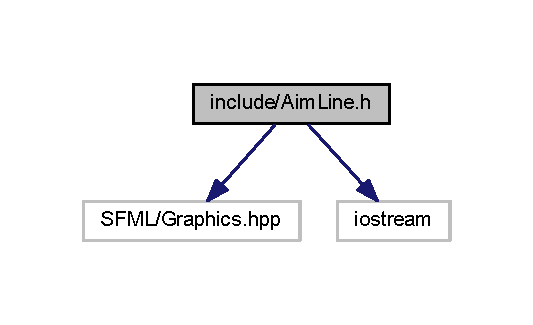
\includegraphics[width=256pt]{_aim_line_8h__incl}
\end{center}
\end{figure}
This graph shows which files directly or indirectly include this file\+:\nopagebreak
\begin{figure}[H]
\begin{center}
\leavevmode
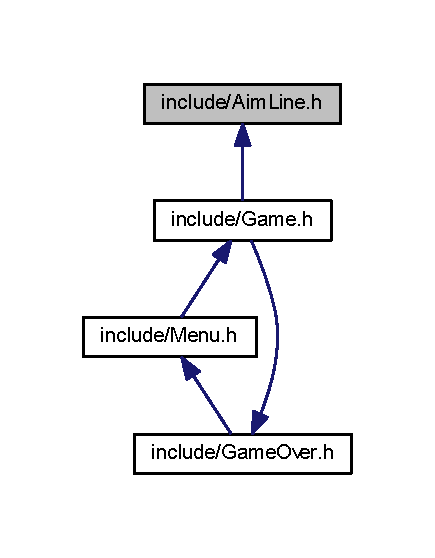
\includegraphics[width=209pt]{_aim_line_8h__dep__incl}
\end{center}
\end{figure}
\subsection*{Classes}
\begin{DoxyCompactItemize}
\item 
class \hyperlink{class_aim_line}{Aim\+Line}
\begin{DoxyCompactList}\small\item\em A class that creates, updates and draws an aiming reticle. \end{DoxyCompactList}\end{DoxyCompactItemize}

\hypertarget{_collision_helper_8h}{}\section{include/\+Collision\+Helper.h File Reference}
\label{_collision_helper_8h}\index{include/\+Collision\+Helper.\+h@{include/\+Collision\+Helper.\+h}}
{\ttfamily \#include $<$S\+F\+M\+L/\+Graphics.\+hpp$>$}\newline
{\ttfamily \#include \char`\"{}Dynamic\+Object.\+h\char`\"{}}\newline
{\ttfamily \#include \char`\"{}Terrain.\+h\char`\"{}}\newline
{\ttfamily \#include \char`\"{}Particle.\+h\char`\"{}}\newline
{\ttfamily \#include $<$iostream$>$}\newline
Include dependency graph for Collision\+Helper.\+h\+:\nopagebreak
\begin{figure}[H]
\begin{center}
\leavevmode
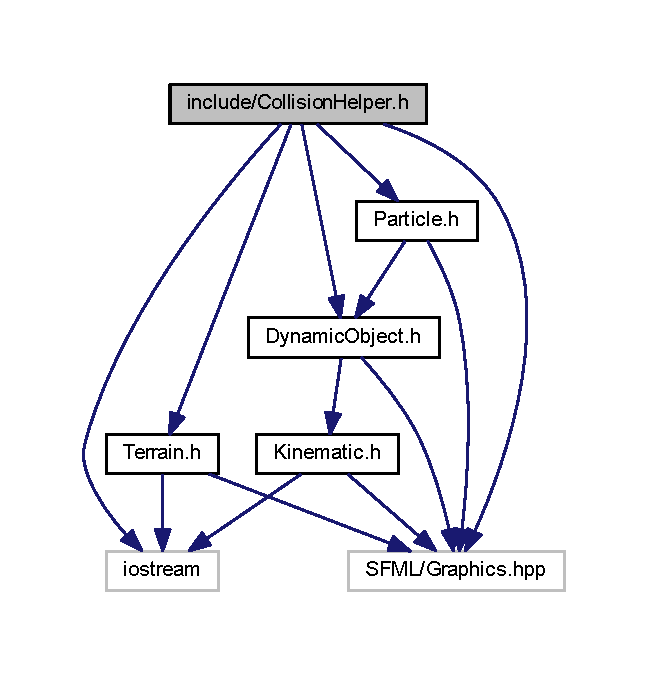
\includegraphics[width=311pt]{_collision_helper_8h__incl}
\end{center}
\end{figure}
This graph shows which files directly or indirectly include this file\+:\nopagebreak
\begin{figure}[H]
\begin{center}
\leavevmode
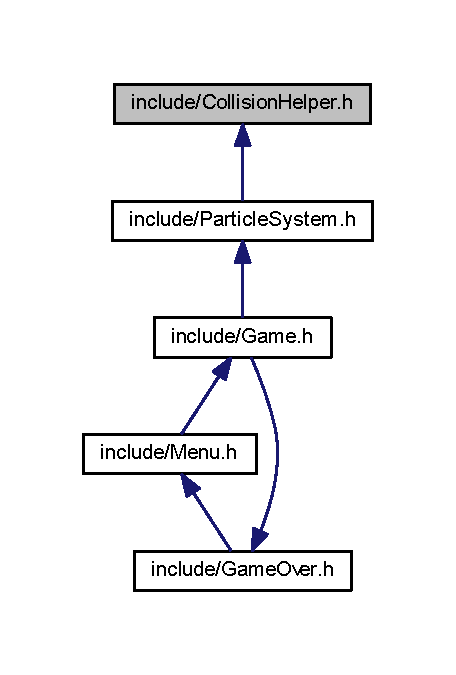
\includegraphics[width=219pt]{_collision_helper_8h__dep__incl}
\end{center}
\end{figure}
\subsection*{Classes}
\begin{DoxyCompactItemize}
\item 
class \hyperlink{class_collision_helper}{Collision\+Helper}
\begin{DoxyCompactList}\small\item\em A class that contains all the relavent collision checking and resolve methods. \end{DoxyCompactList}\end{DoxyCompactItemize}

\hypertarget{_dynamic_object_8h}{}\section{include/\+Dynamic\+Object.h File Reference}
\label{_dynamic_object_8h}\index{include/\+Dynamic\+Object.\+h@{include/\+Dynamic\+Object.\+h}}
{\ttfamily \#include $<$S\+F\+M\+L/\+Graphics.\+hpp$>$}\newline
{\ttfamily \#include \char`\"{}Kinematic.\+h\char`\"{}}\newline
Include dependency graph for Dynamic\+Object.\+h\+:\nopagebreak
\begin{figure}[H]
\begin{center}
\leavevmode
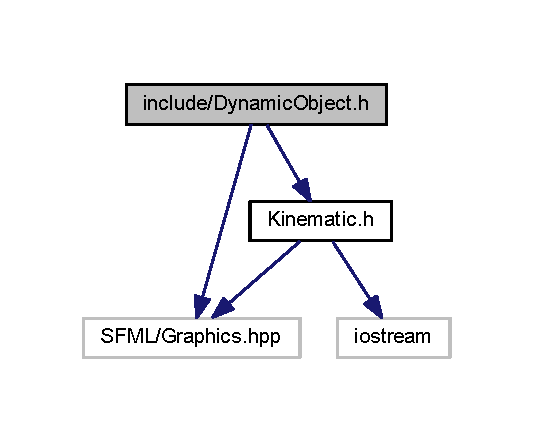
\includegraphics[width=256pt]{_dynamic_object_8h__incl}
\end{center}
\end{figure}
This graph shows which files directly or indirectly include this file\+:\nopagebreak
\begin{figure}[H]
\begin{center}
\leavevmode
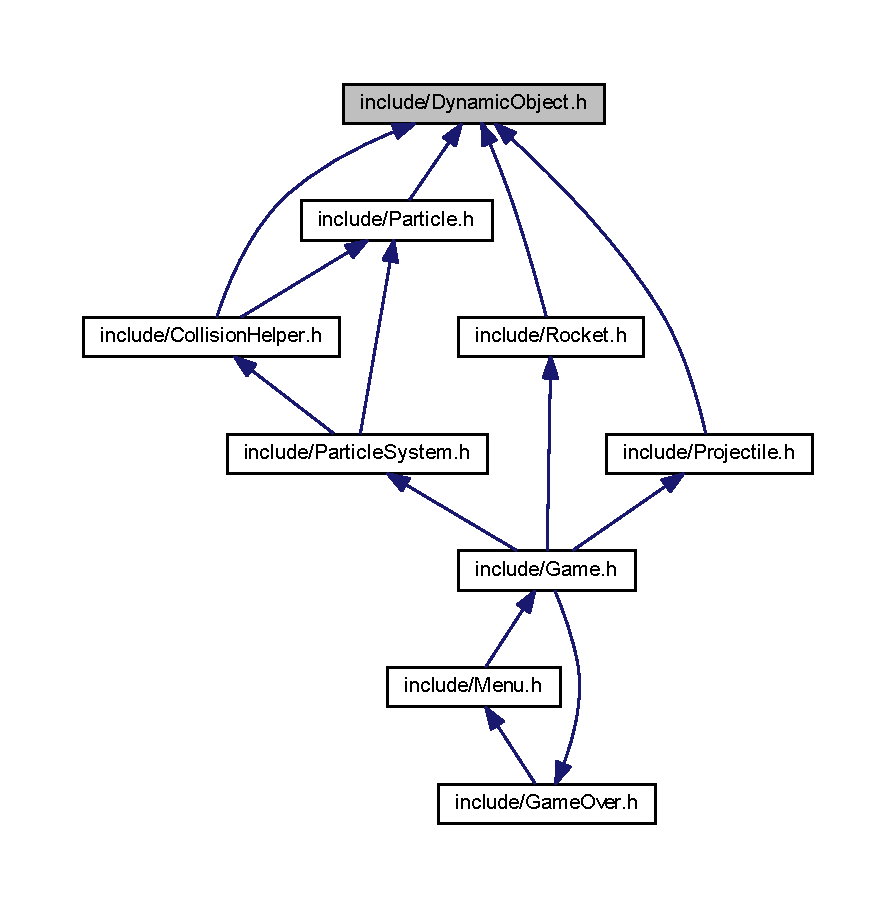
\includegraphics[width=350pt]{_dynamic_object_8h__dep__incl}
\end{center}
\end{figure}
\subsection*{Classes}
\begin{DoxyCompactItemize}
\item 
class \hyperlink{class_dynamic_object}{Dynamic\+Object}
\begin{DoxyCompactList}\small\item\em A kinematic rectangle that can be affected by forces. \end{DoxyCompactList}\end{DoxyCompactItemize}

\hypertarget{_game_8h}{}\section{include/\+Game.h File Reference}
\label{_game_8h}\index{include/\+Game.\+h@{include/\+Game.\+h}}
{\ttfamily \#include $<$S\+F\+M\+L\textbackslash{}\+Graphics.\+hpp$>$}\newline
{\ttfamily \#include $<$iostream$>$}\newline
{\ttfamily \#include $<$list$>$}\newline
{\ttfamily \#include \char`\"{}Texture\+Loader.\+h\char`\"{}}\newline
{\ttfamily \#include \char`\"{}Terrain.\+h\char`\"{}}\newline
{\ttfamily \#include \char`\"{}Particle\+System.\+h\char`\"{}}\newline
{\ttfamily \#include \char`\"{}Rocket.\+h\char`\"{}}\newline
{\ttfamily \#include \char`\"{}Aim\+Line.\+h\char`\"{}}\newline
{\ttfamily \#include \char`\"{}Projectile.\+h\char`\"{}}\newline
{\ttfamily \#include \char`\"{}Scene.\+h\char`\"{}}\newline
{\ttfamily \#include \char`\"{}Game\+Over.\+h\char`\"{}}\newline
Include dependency graph for Game.\+h\+:\nopagebreak
\begin{figure}[H]
\begin{center}
\leavevmode
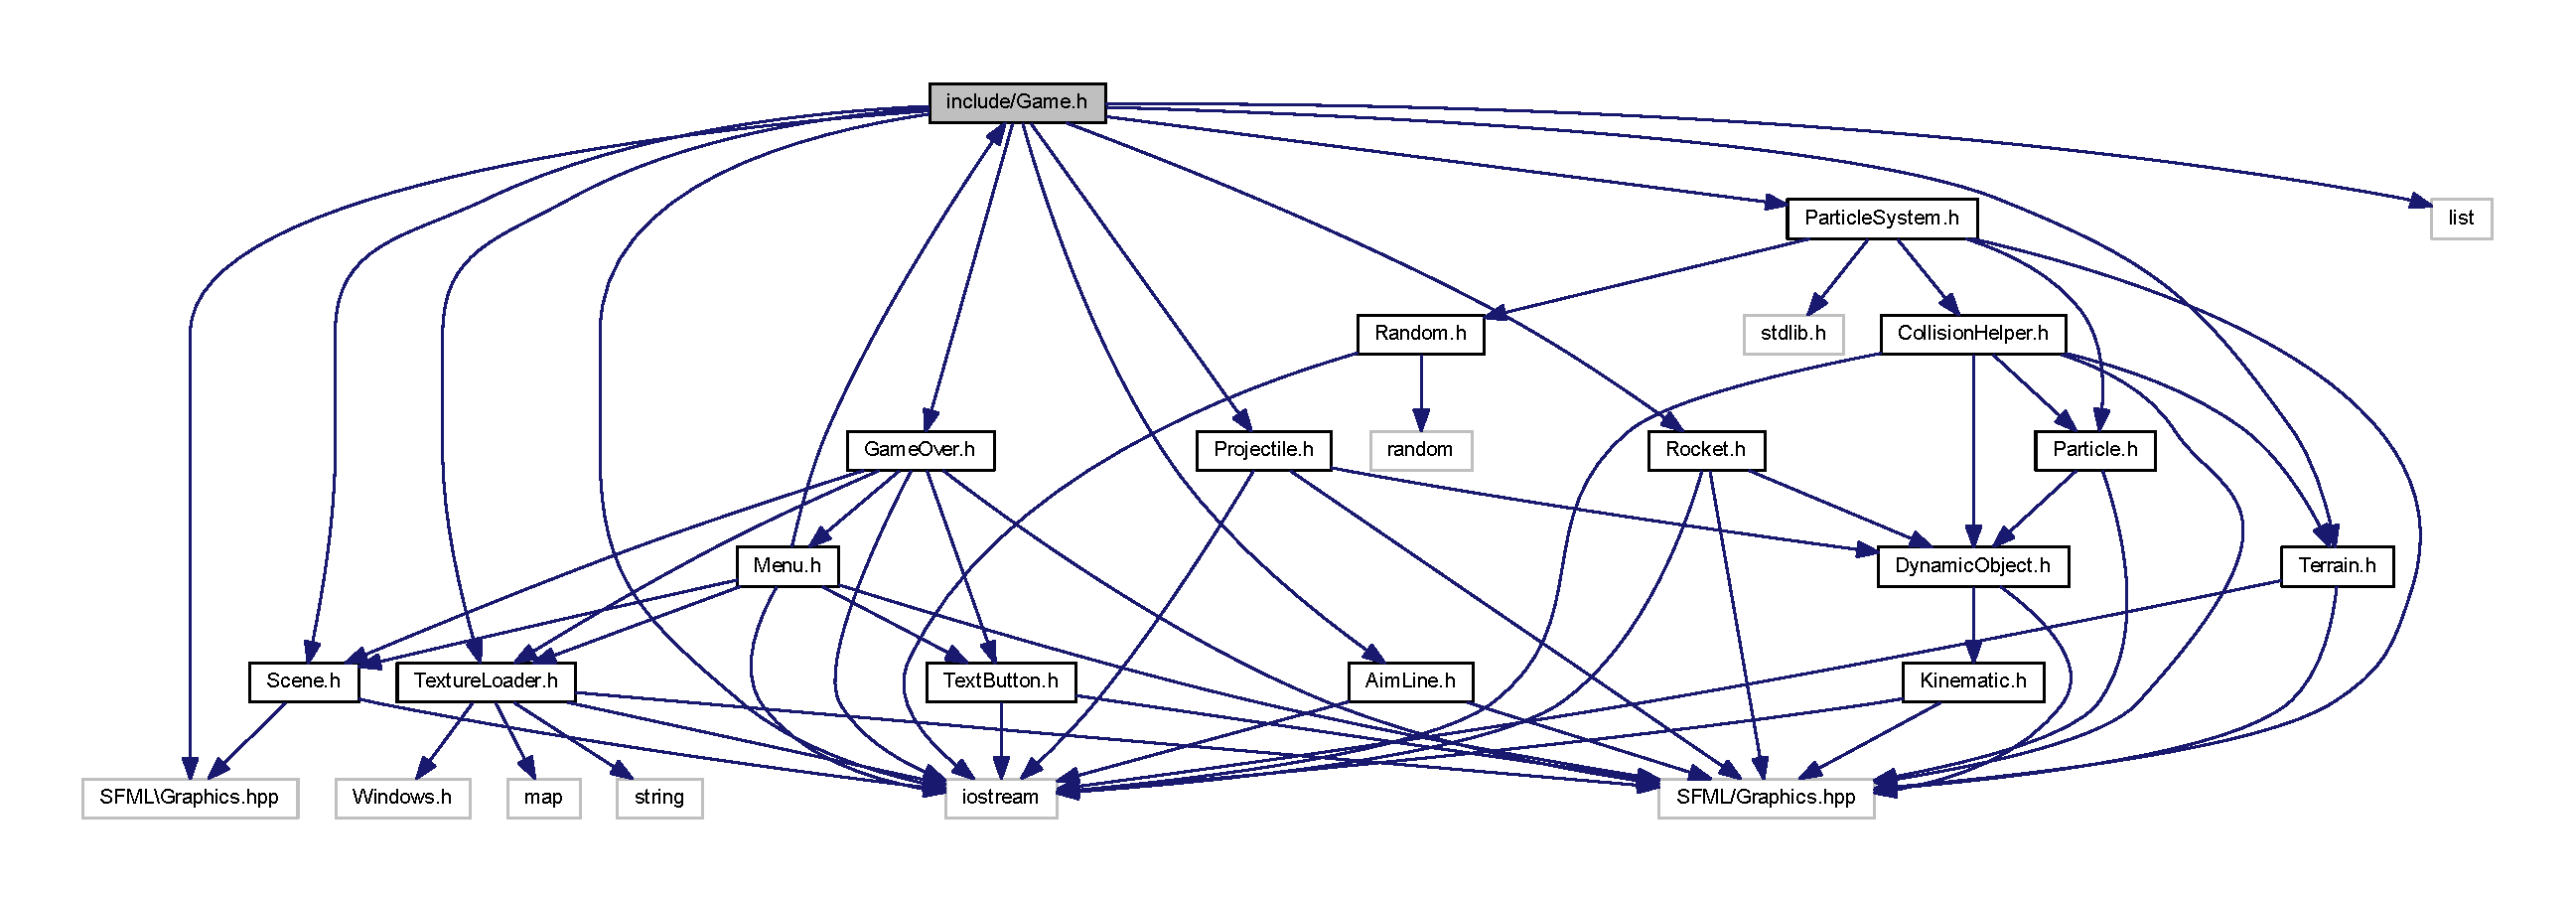
\includegraphics[width=350pt]{_game_8h__incl}
\end{center}
\end{figure}
This graph shows which files directly or indirectly include this file\+:\nopagebreak
\begin{figure}[H]
\begin{center}
\leavevmode
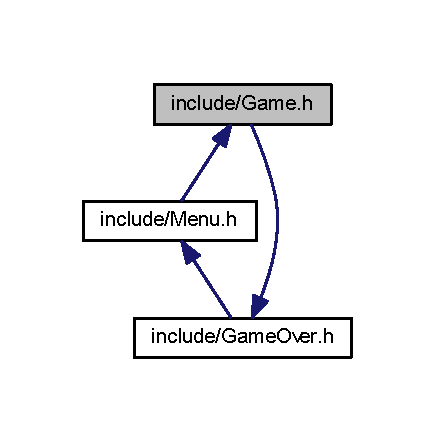
\includegraphics[width=209pt]{_game_8h__dep__incl}
\end{center}
\end{figure}
\subsection*{Classes}
\begin{DoxyCompactItemize}
\item 
class \hyperlink{class_game}{Game}
\begin{DoxyCompactList}\small\item\em A game scene that runs the rocket battle game. \end{DoxyCompactList}\end{DoxyCompactItemize}

\hypertarget{_game_over_8h}{}\section{include/\+Game\+Over.h File Reference}
\label{_game_over_8h}\index{include/\+Game\+Over.\+h@{include/\+Game\+Over.\+h}}
{\ttfamily \#include $<$S\+F\+M\+L/\+Graphics.\+hpp$>$}\newline
{\ttfamily \#include $<$iostream$>$}\newline
{\ttfamily \#include \char`\"{}Scene.\+h\char`\"{}}\newline
{\ttfamily \#include \char`\"{}Texture\+Loader.\+h\char`\"{}}\newline
{\ttfamily \#include \char`\"{}Text\+Button.\+h\char`\"{}}\newline
{\ttfamily \#include \char`\"{}Menu.\+h\char`\"{}}\newline
Include dependency graph for Game\+Over.\+h\+:\nopagebreak
\begin{figure}[H]
\begin{center}
\leavevmode
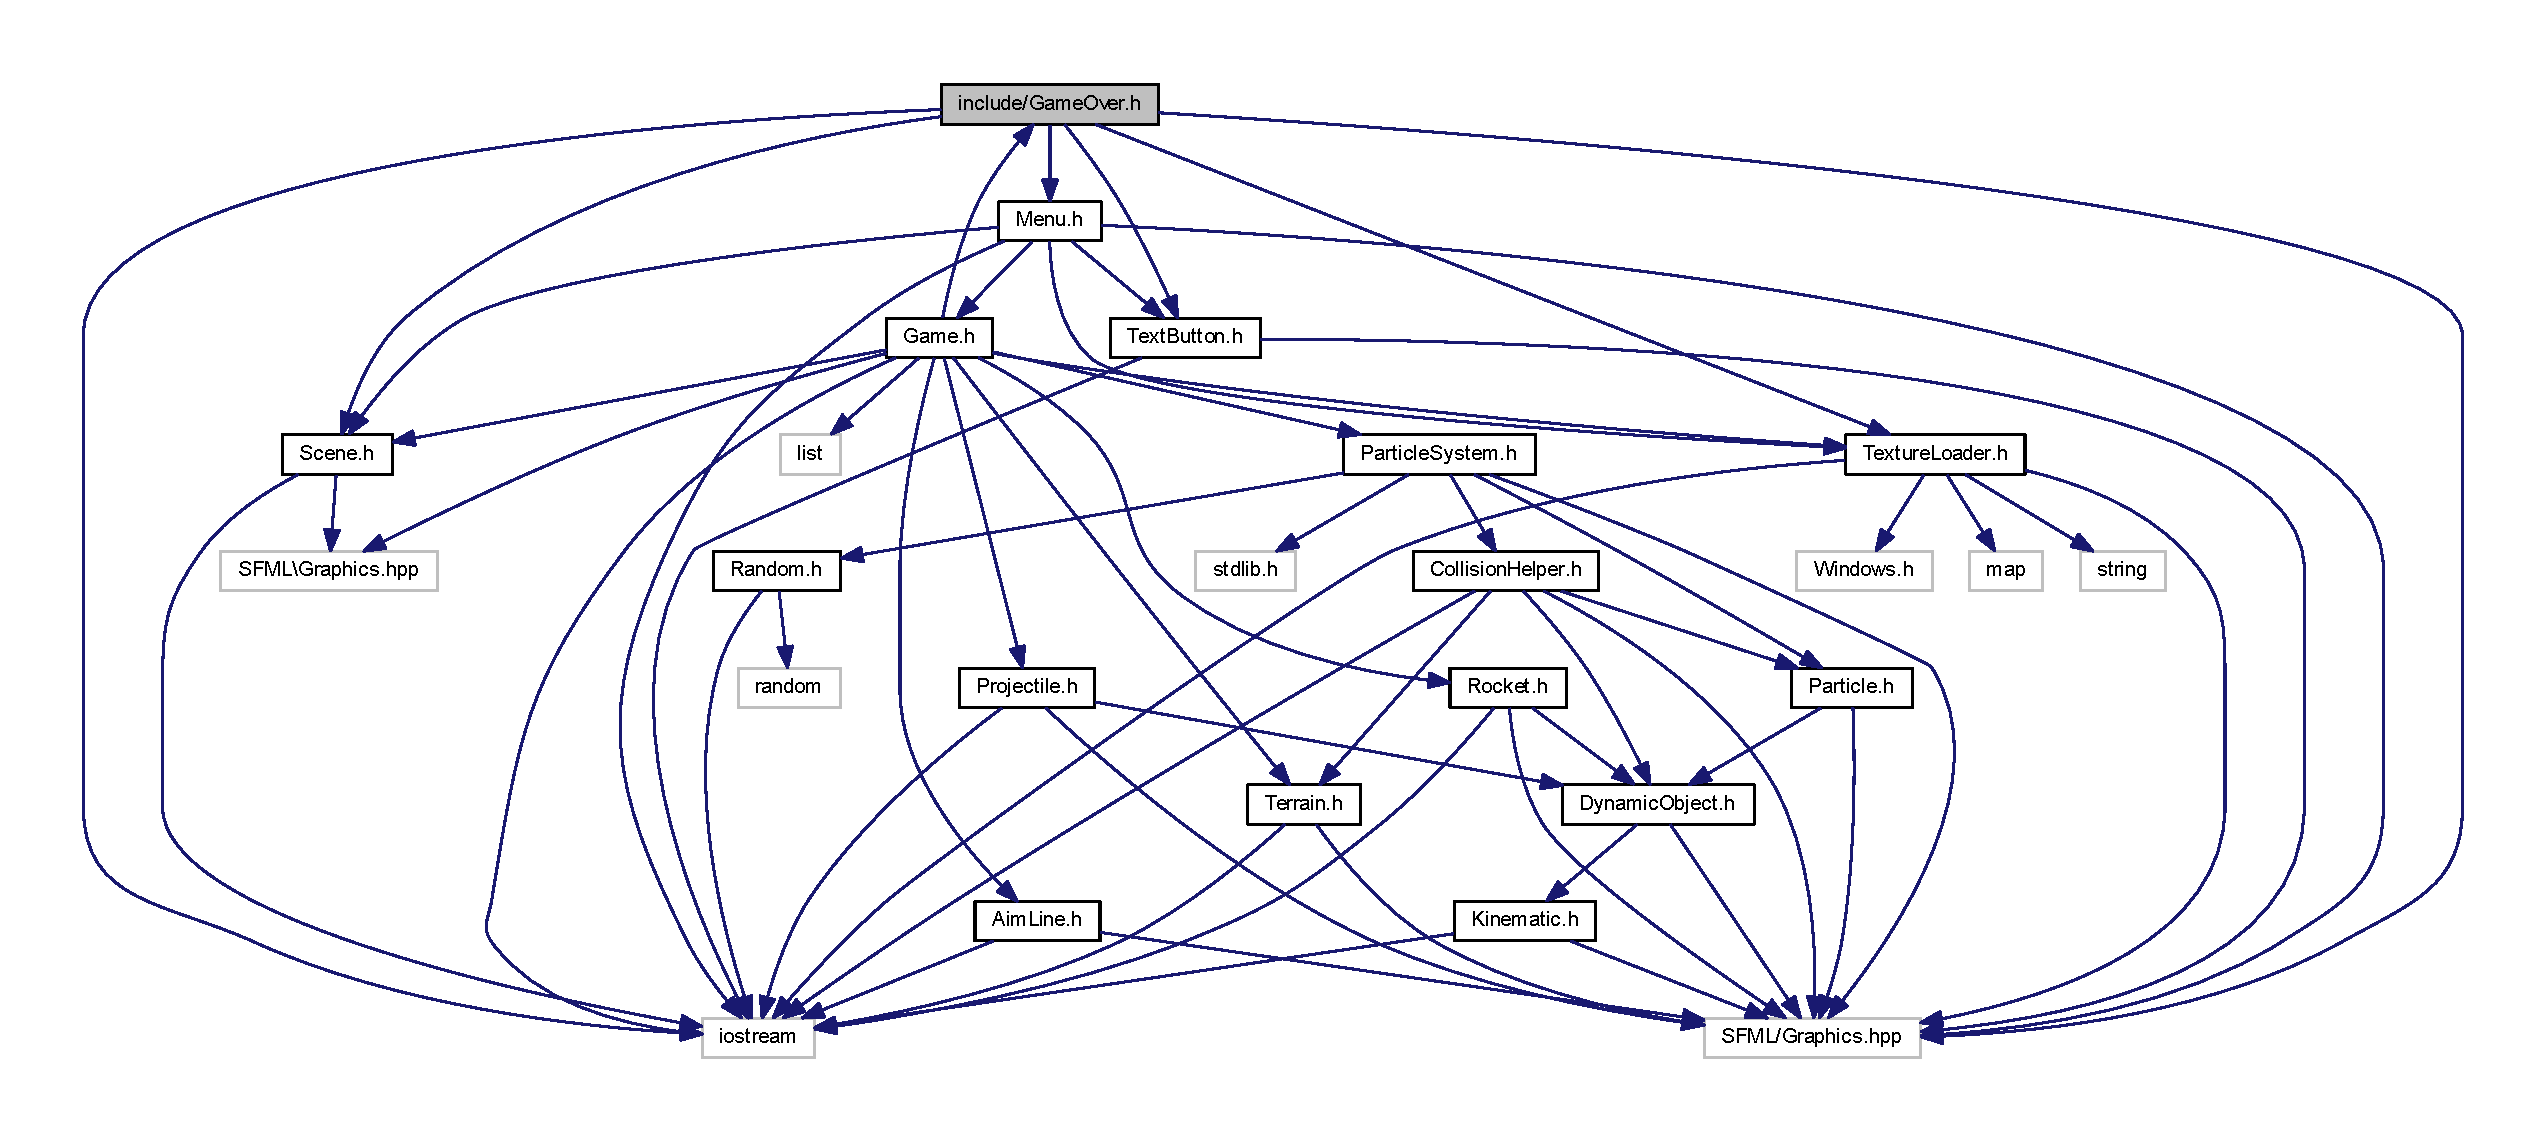
\includegraphics[width=350pt]{_game_over_8h__incl}
\end{center}
\end{figure}
This graph shows which files directly or indirectly include this file\+:\nopagebreak
\begin{figure}[H]
\begin{center}
\leavevmode
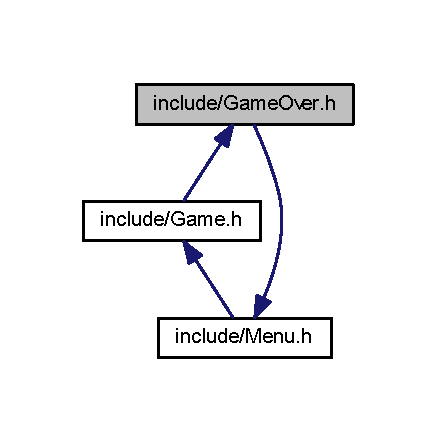
\includegraphics[width=210pt]{_game_over_8h__dep__incl}
\end{center}
\end{figure}
\subsection*{Classes}
\begin{DoxyCompactItemize}
\item 
class \hyperlink{class_game_over}{Game\+Over}
\begin{DoxyCompactList}\small\item\em A menu scene that displays some useful info and allows you to start the game. \end{DoxyCompactList}\end{DoxyCompactItemize}

\hypertarget{_kinematic_8h}{}\section{include/\+Kinematic.h File Reference}
\label{_kinematic_8h}\index{include/\+Kinematic.\+h@{include/\+Kinematic.\+h}}
{\ttfamily \#include $<$S\+F\+M\+L/\+Graphics.\+hpp$>$}\newline
{\ttfamily \#include $<$iostream$>$}\newline
Include dependency graph for Kinematic.\+h\+:\nopagebreak
\begin{figure}[H]
\begin{center}
\leavevmode
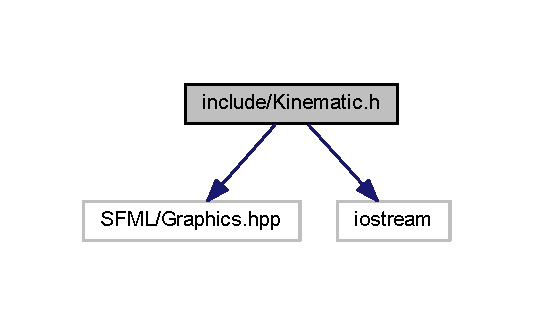
\includegraphics[width=256pt]{_kinematic_8h__incl}
\end{center}
\end{figure}
This graph shows which files directly or indirectly include this file\+:\nopagebreak
\begin{figure}[H]
\begin{center}
\leavevmode
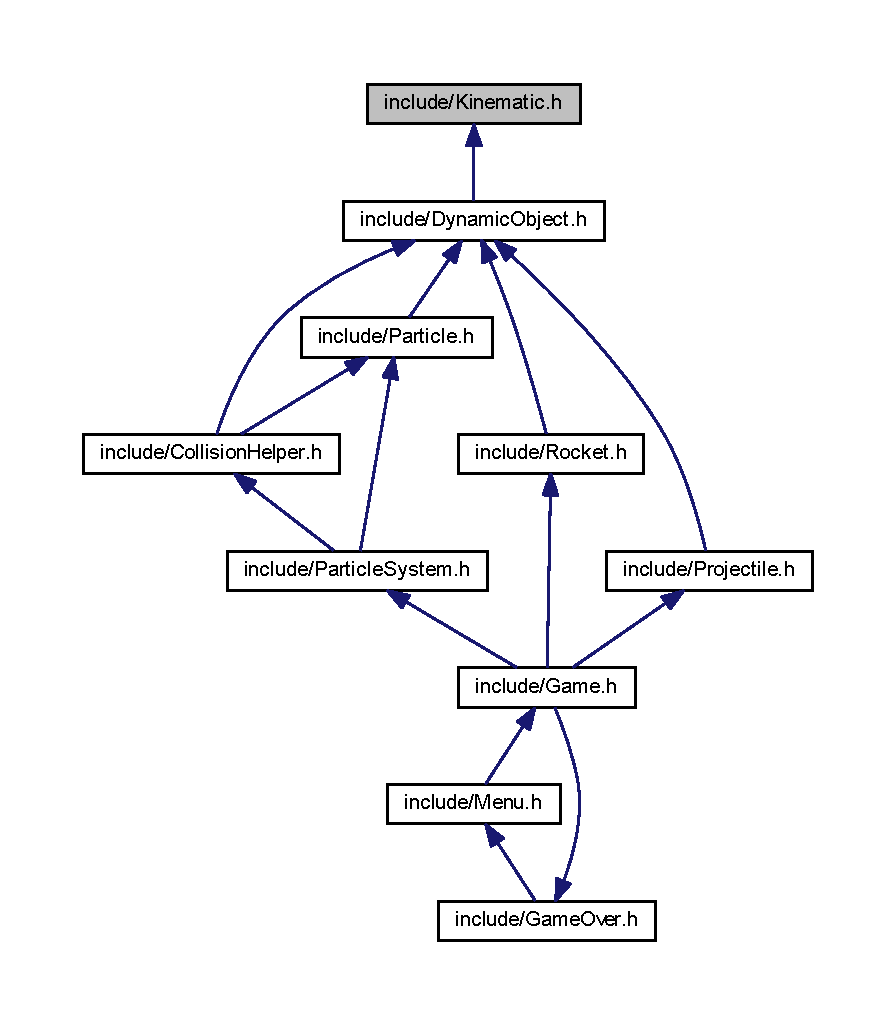
\includegraphics[width=350pt]{_kinematic_8h__dep__incl}
\end{center}
\end{figure}
\subsection*{Classes}
\begin{DoxyCompactItemize}
\item 
class \hyperlink{class_kinematic}{Kinematic}
\begin{DoxyCompactList}\small\item\em A class that provides methods to create motion using position, velocity and acceleration. \end{DoxyCompactList}\end{DoxyCompactItemize}

\hypertarget{_menu_8h}{}\section{include/\+Menu.h File Reference}
\label{_menu_8h}\index{include/\+Menu.\+h@{include/\+Menu.\+h}}
{\ttfamily \#include $<$S\+F\+M\+L/\+Graphics.\+hpp$>$}\newline
{\ttfamily \#include $<$iostream$>$}\newline
{\ttfamily \#include \char`\"{}Scene.\+h\char`\"{}}\newline
{\ttfamily \#include \char`\"{}Texture\+Loader.\+h\char`\"{}}\newline
{\ttfamily \#include \char`\"{}Text\+Button.\+h\char`\"{}}\newline
{\ttfamily \#include \char`\"{}Game.\+h\char`\"{}}\newline
Include dependency graph for Menu.\+h\+:\nopagebreak
\begin{figure}[H]
\begin{center}
\leavevmode
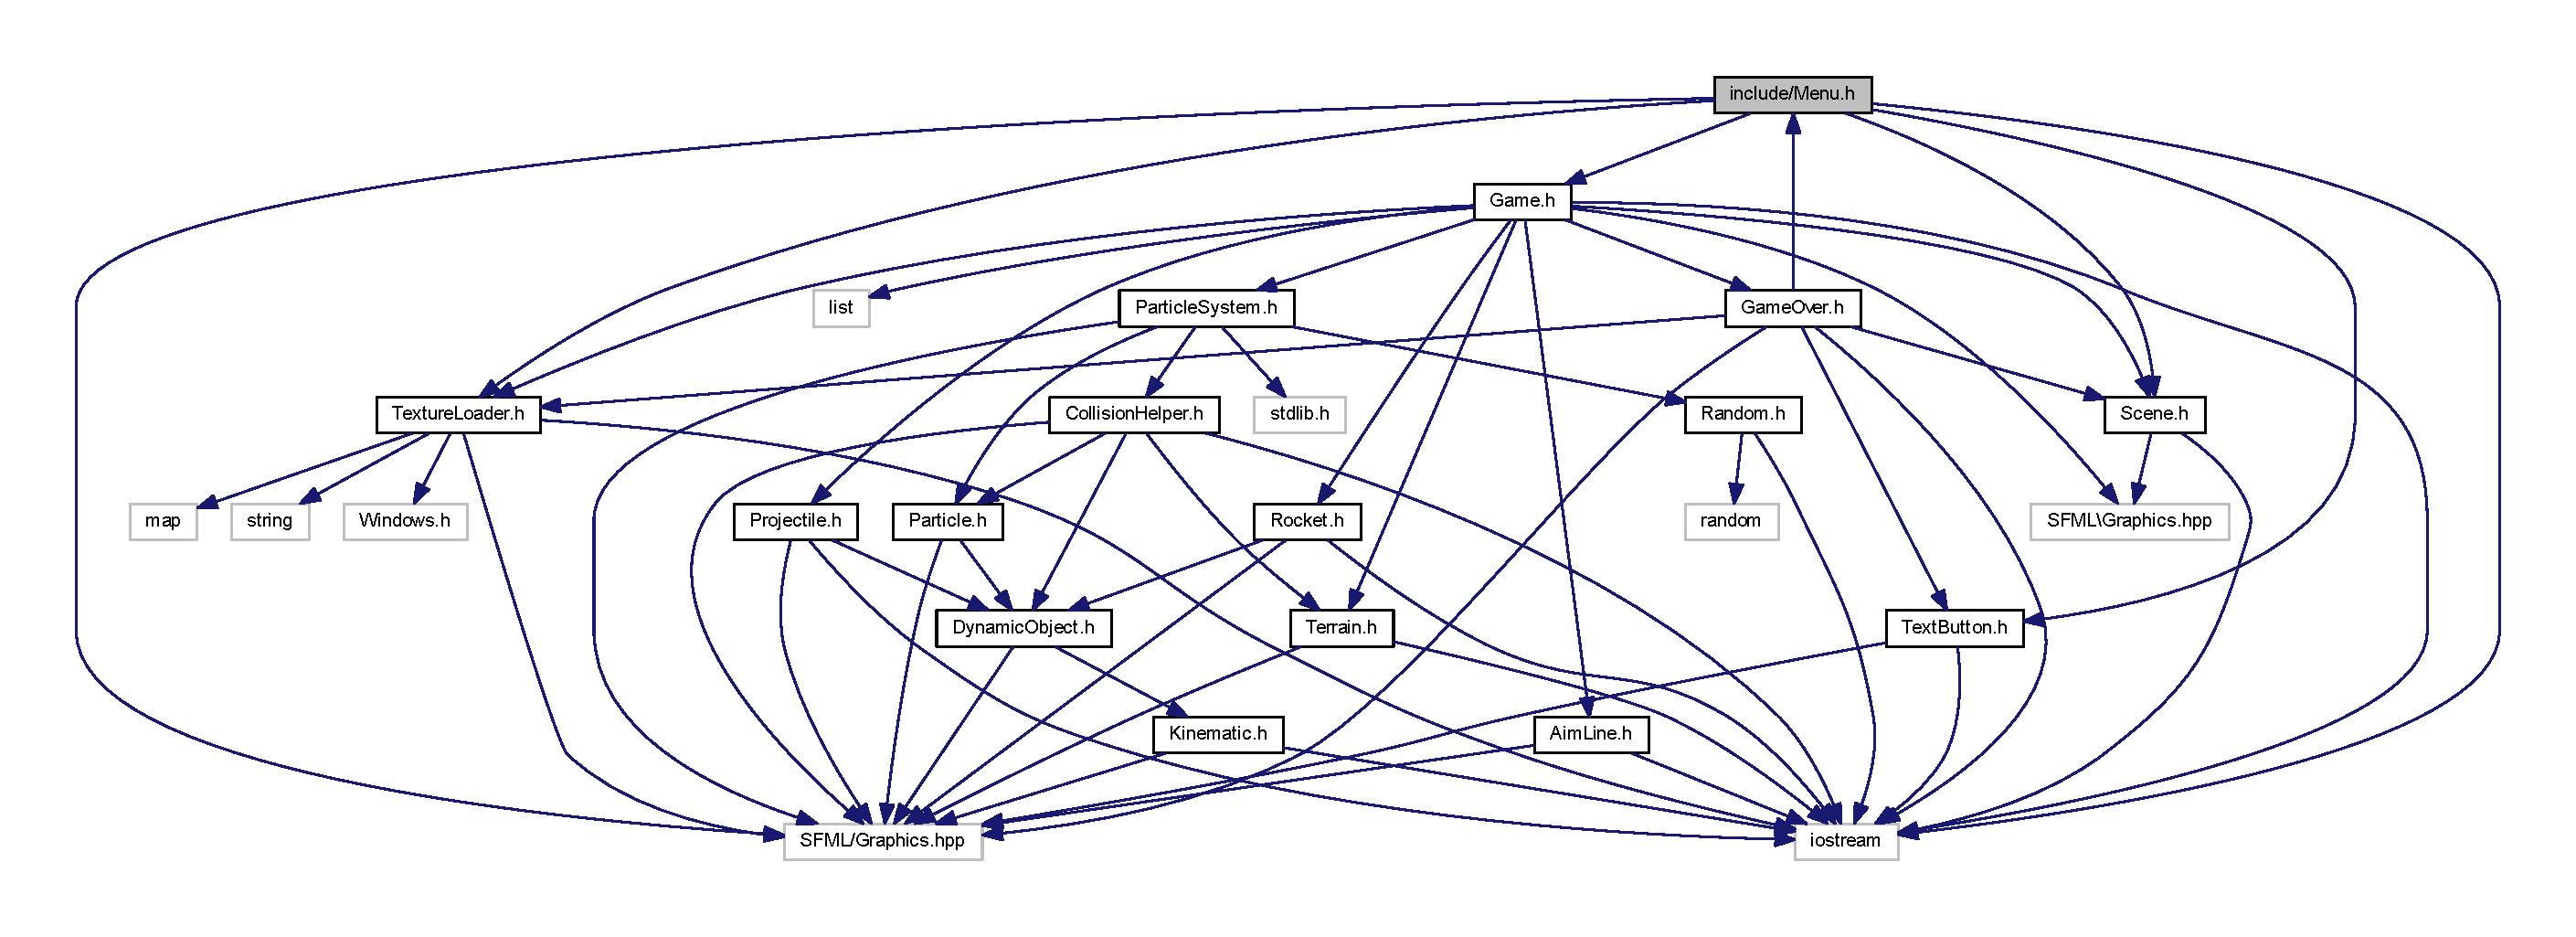
\includegraphics[width=350pt]{_menu_8h__incl}
\end{center}
\end{figure}
This graph shows which files directly or indirectly include this file\+:\nopagebreak
\begin{figure}[H]
\begin{center}
\leavevmode
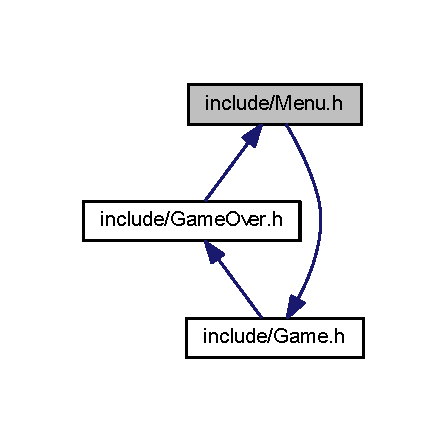
\includegraphics[width=215pt]{_menu_8h__dep__incl}
\end{center}
\end{figure}
\subsection*{Classes}
\begin{DoxyCompactItemize}
\item 
class \hyperlink{class_menu}{Menu}
\begin{DoxyCompactList}\small\item\em A menu scene that displays some useful info and allows you to start the game. \end{DoxyCompactList}\end{DoxyCompactItemize}

\hypertarget{_particle_8h}{}\section{include/\+Particle.h File Reference}
\label{_particle_8h}\index{include/\+Particle.\+h@{include/\+Particle.\+h}}
{\ttfamily \#include $<$S\+F\+M\+L/\+Graphics.\+hpp$>$}\newline
{\ttfamily \#include \char`\"{}Dynamic\+Object.\+h\char`\"{}}\newline
Include dependency graph for Particle.\+h\+:\nopagebreak
\begin{figure}[H]
\begin{center}
\leavevmode
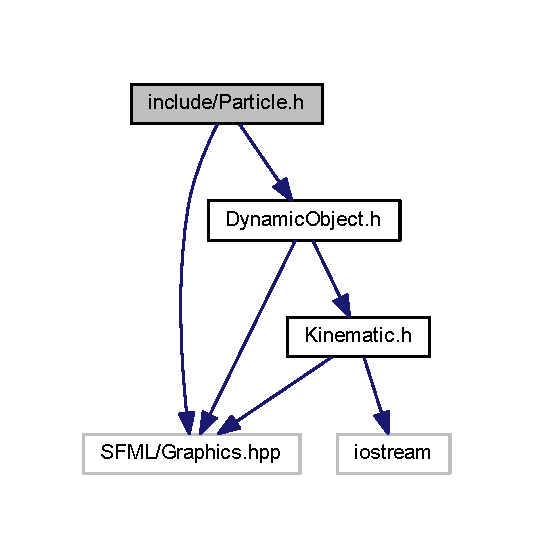
\includegraphics[width=256pt]{_particle_8h__incl}
\end{center}
\end{figure}
This graph shows which files directly or indirectly include this file\+:\nopagebreak
\begin{figure}[H]
\begin{center}
\leavevmode
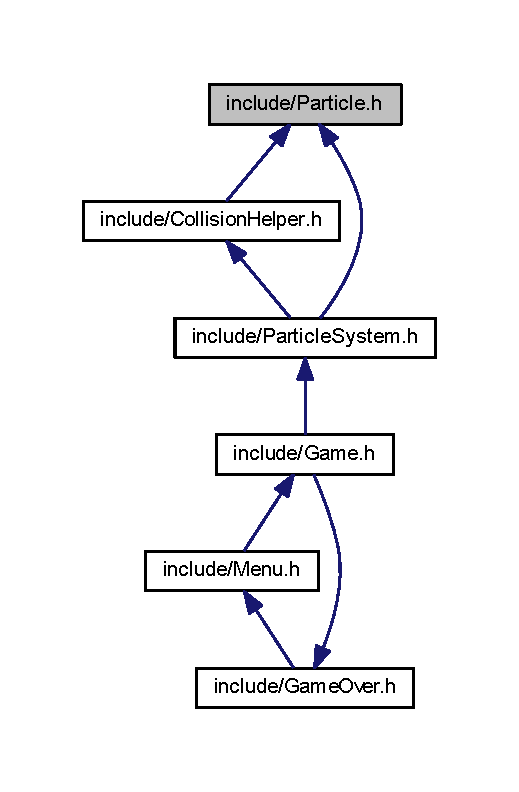
\includegraphics[width=249pt]{_particle_8h__dep__incl}
\end{center}
\end{figure}
\subsection*{Classes}
\begin{DoxyCompactItemize}
\item 
class \hyperlink{class_particle}{Particle}
\begin{DoxyCompactList}\small\item\em A dynamic object that keeps track of how long it exists for and its previous position. \end{DoxyCompactList}\end{DoxyCompactItemize}

\hypertarget{_particle_system_8h}{}\section{include/\+Particle\+System.h File Reference}
\label{_particle_system_8h}\index{include/\+Particle\+System.\+h@{include/\+Particle\+System.\+h}}
{\ttfamily \#include $<$S\+F\+M\+L/\+Graphics.\+hpp$>$}\newline
{\ttfamily \#include \char`\"{}Particle.\+h\char`\"{}}\newline
{\ttfamily \#include $<$stdlib.\+h$>$}\newline
{\ttfamily \#include \char`\"{}Random.\+h\char`\"{}}\newline
{\ttfamily \#include \char`\"{}Collision\+Helper.\+h\char`\"{}}\newline
Include dependency graph for Particle\+System.\+h\+:\nopagebreak
\begin{figure}[H]
\begin{center}
\leavevmode
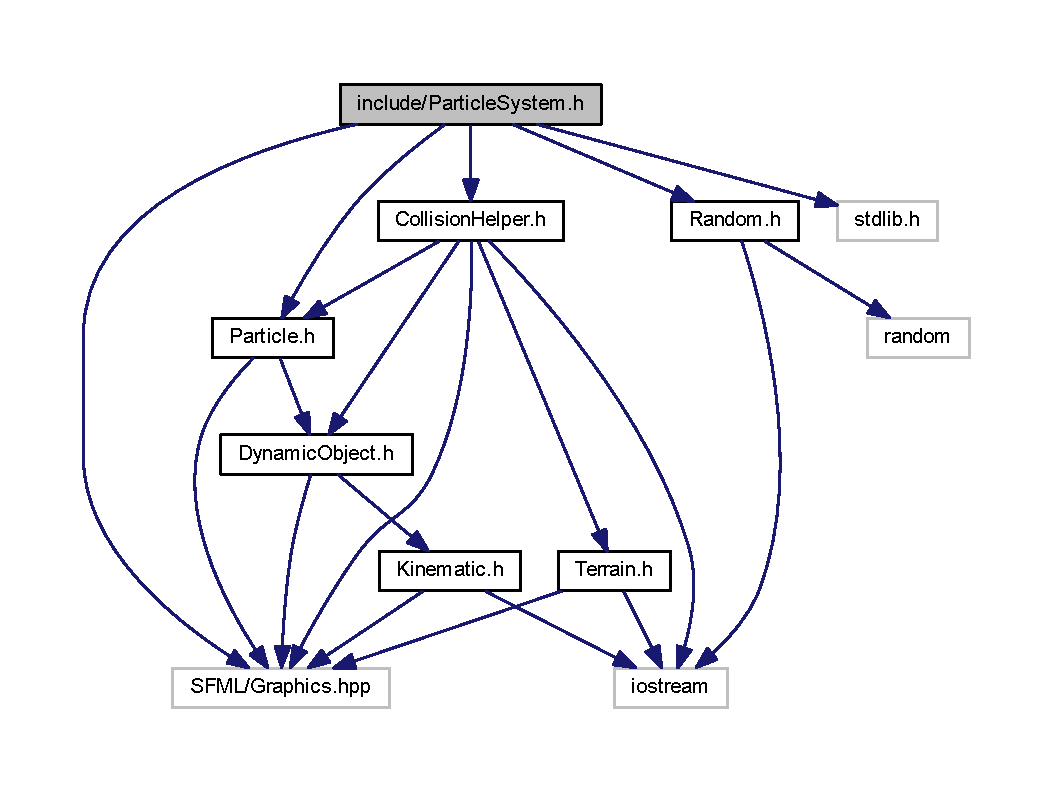
\includegraphics[width=350pt]{_particle_system_8h__incl}
\end{center}
\end{figure}
This graph shows which files directly or indirectly include this file\+:\nopagebreak
\begin{figure}[H]
\begin{center}
\leavevmode
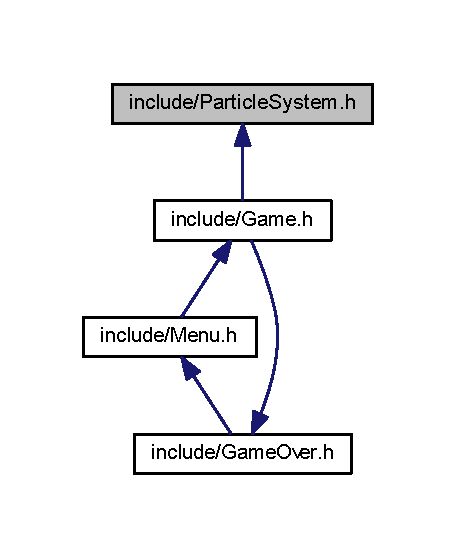
\includegraphics[width=219pt]{_particle_system_8h__dep__incl}
\end{center}
\end{figure}
\subsection*{Classes}
\begin{DoxyCompactItemize}
\item 
class \hyperlink{class_particle_system}{Particle\+System}
\begin{DoxyCompactList}\small\item\em A class that handles updating particles and drawing their respective vertices. \end{DoxyCompactList}\end{DoxyCompactItemize}

\hypertarget{_projectile_8h}{}\section{include/\+Projectile.h File Reference}
\label{_projectile_8h}\index{include/\+Projectile.\+h@{include/\+Projectile.\+h}}
{\ttfamily \#include $<$S\+F\+M\+L/\+Graphics.\+hpp$>$}\newline
{\ttfamily \#include $<$iostream$>$}\newline
{\ttfamily \#include \char`\"{}Dynamic\+Object.\+h\char`\"{}}\newline
Include dependency graph for Projectile.\+h\+:\nopagebreak
\begin{figure}[H]
\begin{center}
\leavevmode
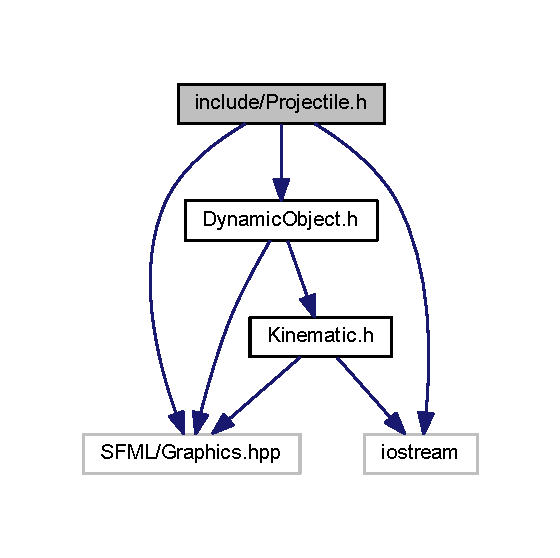
\includegraphics[width=269pt]{_projectile_8h__incl}
\end{center}
\end{figure}
This graph shows which files directly or indirectly include this file\+:\nopagebreak
\begin{figure}[H]
\begin{center}
\leavevmode
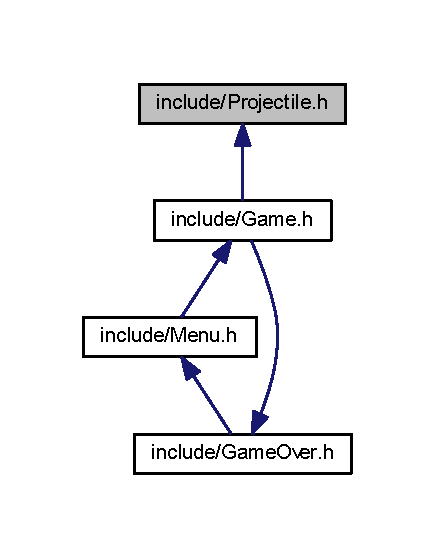
\includegraphics[width=209pt]{_projectile_8h__dep__incl}
\end{center}
\end{figure}
\subsection*{Classes}
\begin{DoxyCompactItemize}
\item 
class \hyperlink{class_projectile}{Projectile}
\begin{DoxyCompactList}\small\item\em A dynamic object that has damage. \end{DoxyCompactList}\end{DoxyCompactItemize}

\hypertarget{_random_8h}{}\section{include/\+Random.h File Reference}
\label{_random_8h}\index{include/\+Random.\+h@{include/\+Random.\+h}}
{\ttfamily \#include $<$iostream$>$}\newline
{\ttfamily \#include $<$random$>$}\newline
Include dependency graph for Random.\+h\+:\nopagebreak
\begin{figure}[H]
\begin{center}
\leavevmode
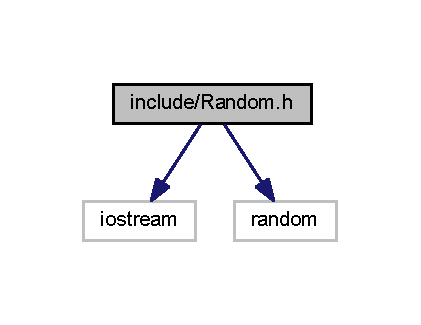
\includegraphics[width=202pt]{_random_8h__incl}
\end{center}
\end{figure}
This graph shows which files directly or indirectly include this file\+:\nopagebreak
\begin{figure}[H]
\begin{center}
\leavevmode
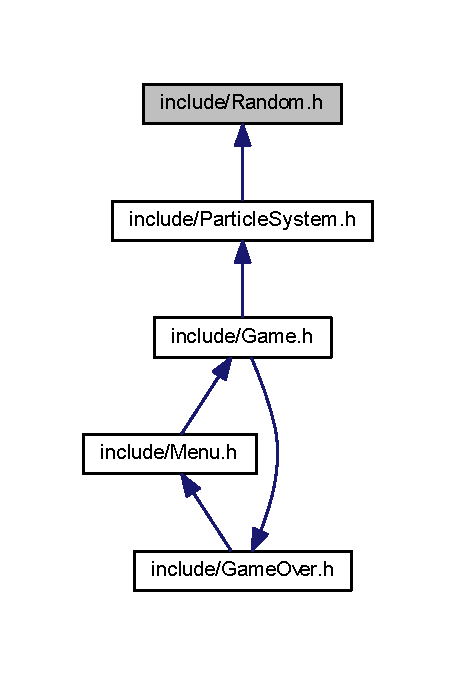
\includegraphics[width=219pt]{_random_8h__dep__incl}
\end{center}
\end{figure}
\subsection*{Classes}
\begin{DoxyCompactItemize}
\item 
class \hyperlink{class_random}{Random}
\begin{DoxyCompactList}\small\item\em Singleton class that holds random number engines. \end{DoxyCompactList}\end{DoxyCompactItemize}

\hypertarget{_rocket_8h}{}\section{include/\+Rocket.h File Reference}
\label{_rocket_8h}\index{include/\+Rocket.\+h@{include/\+Rocket.\+h}}
{\ttfamily \#include $<$S\+F\+M\+L/\+Graphics.\+hpp$>$}\newline
{\ttfamily \#include $<$iostream$>$}\newline
{\ttfamily \#include \char`\"{}Dynamic\+Object.\+h\char`\"{}}\newline
Include dependency graph for Rocket.\+h\+:\nopagebreak
\begin{figure}[H]
\begin{center}
\leavevmode
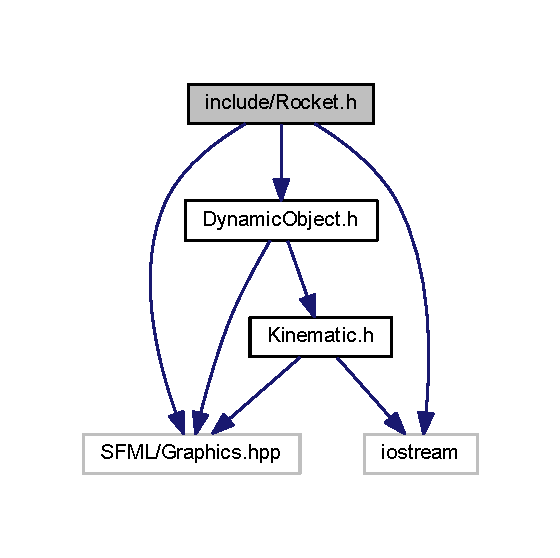
\includegraphics[width=269pt]{_rocket_8h__incl}
\end{center}
\end{figure}
This graph shows which files directly or indirectly include this file\+:\nopagebreak
\begin{figure}[H]
\begin{center}
\leavevmode
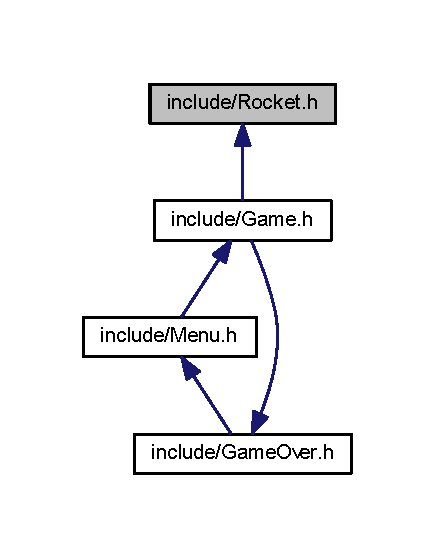
\includegraphics[width=209pt]{_rocket_8h__dep__incl}
\end{center}
\end{figure}
\subsection*{Classes}
\begin{DoxyCompactItemize}
\item 
class \hyperlink{class_rocket}{Rocket}
\begin{DoxyCompactList}\small\item\em A playable rocket class that keeps track of fuel and life. \end{DoxyCompactList}\end{DoxyCompactItemize}

\hypertarget{_scene_8h}{}\section{include/\+Scene.h File Reference}
\label{_scene_8h}\index{include/\+Scene.\+h@{include/\+Scene.\+h}}
{\ttfamily \#include $<$S\+F\+M\+L\textbackslash{}\+Graphics.\+hpp$>$}\newline
{\ttfamily \#include $<$iostream$>$}\newline
Include dependency graph for Scene.\+h\+:\nopagebreak
\begin{figure}[H]
\begin{center}
\leavevmode
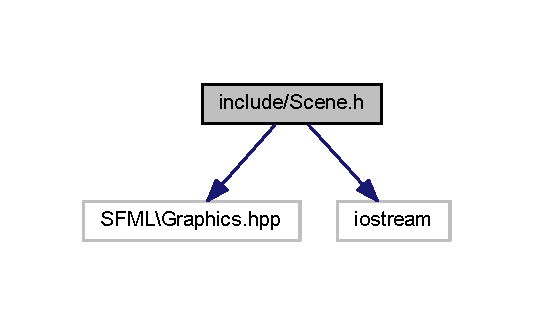
\includegraphics[width=256pt]{_scene_8h__incl}
\end{center}
\end{figure}
This graph shows which files directly or indirectly include this file\+:\nopagebreak
\begin{figure}[H]
\begin{center}
\leavevmode
\includegraphics[width=244pt]{_scene_8h__dep__incl}
\end{center}
\end{figure}
\subsection*{Classes}
\begin{DoxyCompactItemize}
\item 
class \hyperlink{class_scene}{Scene}
\begin{DoxyCompactList}\small\item\em A class that provides late binding methods for an interactable screen e.\+g. a game or a menu. \end{DoxyCompactList}\end{DoxyCompactItemize}

\hypertarget{_terrain_8h}{}\section{include/\+Terrain.h File Reference}
\label{_terrain_8h}\index{include/\+Terrain.\+h@{include/\+Terrain.\+h}}
{\ttfamily \#include $<$S\+F\+M\+L/\+Graphics.\+hpp$>$}\newline
\subsection*{Classes}
\begin{DoxyCompactItemize}
\item 
class \hyperlink{class_terrain}{Terrain}
\end{DoxyCompactItemize}

\hypertarget{_text_button_8h}{}\section{include/\+Text\+Button.h File Reference}
\label{_text_button_8h}\index{include/\+Text\+Button.\+h@{include/\+Text\+Button.\+h}}
{\ttfamily \#include $<$S\+F\+M\+L/\+Graphics.\+hpp$>$}\newline
{\ttfamily \#include $<$iostream$>$}\newline
Include dependency graph for Text\+Button.\+h\+:\nopagebreak
\begin{figure}[H]
\begin{center}
\leavevmode
\includegraphics[width=256pt]{_text_button_8h__incl}
\end{center}
\end{figure}
This graph shows which files directly or indirectly include this file\+:\nopagebreak
\begin{figure}[H]
\begin{center}
\leavevmode
\includegraphics[width=245pt]{_text_button_8h__dep__incl}
\end{center}
\end{figure}
\subsection*{Classes}
\begin{DoxyCompactItemize}
\item 
class \hyperlink{class_text_button}{Text\+Button}
\begin{DoxyCompactList}\small\item\em A Wrapper class for sf\+::\+Text and sf\+::\+Font that adds a mosue over checker. \end{DoxyCompactList}\end{DoxyCompactItemize}

\hypertarget{_texture_loader_8h}{}\section{include/\+Texture\+Loader.h File Reference}
\label{_texture_loader_8h}\index{include/\+Texture\+Loader.\+h@{include/\+Texture\+Loader.\+h}}
{\ttfamily \#include $<$S\+F\+M\+L/\+Graphics.\+hpp$>$}\newline
{\ttfamily \#include $<$map$>$}\newline
{\ttfamily \#include $<$string$>$}\newline
{\ttfamily \#include $<$Windows.\+h$>$}\newline
{\ttfamily \#include $<$iostream$>$}\newline
Include dependency graph for Texture\+Loader.\+h\+:\nopagebreak
\begin{figure}[H]
\begin{center}
\leavevmode
\includegraphics[width=350pt]{_texture_loader_8h__incl}
\end{center}
\end{figure}
This graph shows which files directly or indirectly include this file\+:\nopagebreak
\begin{figure}[H]
\begin{center}
\leavevmode
\includegraphics[width=244pt]{_texture_loader_8h__dep__incl}
\end{center}
\end{figure}
\subsection*{Classes}
\begin{DoxyCompactItemize}
\item 
class \hyperlink{class_texture_loader}{Texture\+Loader}
\begin{DoxyCompactList}\small\item\em A singleton loader class that prevents any unnecessary copying of potentially large texture files. \end{DoxyCompactList}\end{DoxyCompactItemize}

%--- End generated contents ---

% Index
\backmatter
\newpage
\phantomsection
\clearemptydoublepage
\addcontentsline{toc}{chapter}{Index}
\printindex

\end{document}
